\documentclass[a4paper,11pt]{book}
%\documentclass[a4paper,twoside,11pt,titlepage]{book}
\usepackage{listings}
\usepackage[utf8]{inputenc}
\usepackage[spanish]{babel}
\usepackage{amsmath}

\usepackage{float}


% \usepackage[style=list, number=none]{glossary} %
%\usepackage{titlesec}
%\usepackage{pailatino}

\decimalpoint
\usepackage{dcolumn}
\newcolumntype{.}{D{.}{\esperiod}{-1}}
\makeatletter
\addto\shorthandsspanish{\let\esperiod\es@period@code}
\makeatother


%\usepackage[chapter]{algorithm}
\RequirePackage{verbatim}
%\RequirePackage[Glenn]{fncychap}
\usepackage{fancyhdr}
\usepackage{graphicx}
\usepackage{afterpage}

\usepackage{longtable}

\usepackage[pdfborder={000}]{hyperref} %referencia

% ********************************************************************
% Re-usable information
% ********************************************************************
\newcommand{\myTitle}{Aplicación de IA para la Visualización de Datos Clínicos\xspace}
\newcommand{\myDegree}{Grado en ...\xspace}
\newcommand{\myName}{Nombre Apllido1 Apellido2 (alumno)\xspace}
\newcommand{\myProf}{Nombre Apllido1 Apellido2 (tutor1)\xspace}
\newcommand{\myOtherProf}{Nombre Apllido1 Apellido2 (tutor2)\xspace}
%\newcommand{\mySupervisor}{Put name here\xspace}
\newcommand{\myFaculty}{Escuela Técnica Superior de Ingenierías Informática y de
Telecomunicación\xspace}
\newcommand{\myFacultyShort}{E.T.S. de Ingenierías Informática y de
Telecomunicación\xspace}
\newcommand{\myDepartment}{Departamento de ...\xspace}
\newcommand{\myUni}{\protect{Universidad de Granada}\xspace}
\newcommand{\myLocation}{Granada\xspace}
\newcommand{\myTime}{\today\xspace}
\newcommand{\myVersion}{Version 0.1\xspace}


\hypersetup{
pdfauthor = {\myName (email (en) ugr (punto) es)},
pdftitle = {\myTitle},
pdfsubject = {},
pdfkeywords = {palabra_clave1, palabra_clave2, palabra_clave3, ...},
pdfcreator = {LaTeX con el paquete ....},
pdfproducer = {pdflatex}
}

%\hyphenation{}


%\usepackage{doxygen/doxygen}
%\usepackage{pdfpages}
\usepackage{url}
\usepackage{colortbl,longtable}
\usepackage[stable]{footmisc}
%\usepackage{index}

%\makeindex
%\usepackage[style=long, cols=2,border=plain,toc=true,number=none]{glossary}
% \makeglossary

% Definición de comandos que me son tiles:
%\renewcommand{\indexname}{Índice alfabético}
%\renewcommand{\glossaryname}{Glosario}

\pagestyle{fancy}
\fancyhf{}
\fancyhead[LO]{\leftmark}
\fancyhead[RE]{\rightmark}
\fancyhead[RO,LE]{\textbf{\thepage}}
\renewcommand{\chaptermark}[1]{\markboth{\textbf{\footnotesize #1}}{}}
\renewcommand{\sectionmark}[1]{\markright{\textbf{\footnotesize \thesection. #1}}}

\setlength{\headheight}{1.5\headheight}

\newcommand{\HRule}{\rule{\linewidth}{0.5mm}}
%Definimos los tipos teorema, ejemplo y definición podremos usar estos tipos
%simplemente poniendo \begin{teorema} \end{teorema} ...
\newtheorem{teorema}{Teorema}[chapter]
\newtheorem{ejemplo}{Ejemplo}[chapter]
\newtheorem{definicion}{Definición}[chapter]

\definecolor{gray97}{gray}{.97}
\definecolor{gray75}{gray}{.75}
\definecolor{gray45}{gray}{.45}
\definecolor{gray30}{gray}{.94}

\lstset{ frame=Ltb,
     framerule=0.5pt,
     aboveskip=0.5cm,
     framextopmargin=3pt,
     framexbottommargin=3pt,
     framexleftmargin=0.1cm,
     framesep=0pt,
     rulesep=.4pt,
     backgroundcolor=\color{gray97},
     rulesepcolor=\color{black},
     %
     stringstyle=\ttfamily,
     showstringspaces = false,
     basicstyle=\scriptsize\ttfamily,
     commentstyle=\color{gray45},
     keywordstyle=\bfseries,
     %
     numbers=left,
     numbersep=6pt,
     numberstyle=\tiny,
     numberfirstline = false,
     breaklines=true,
   }
 
% minimizar fragmentado de listados
\lstnewenvironment{listing}[1][]
   {\lstset{#1}\pagebreak[0]}{\pagebreak[0]}

\lstdefinestyle{CodigoC}
   {
	basicstyle=\scriptsize,
	frame=single,
	language=C,
	numbers=left
   }
\lstdefinestyle{CodigoC++}
   {
	basicstyle=\small,
	frame=single,
	backgroundcolor=\color{gray30},
	language=C++,
	numbers=left
   }

 
\lstdefinestyle{Consola}
   {basicstyle=\scriptsize\bf\ttfamily,
    backgroundcolor=\color{gray30},
    frame=single,
    numbers=none
   }


\newcommand{\bigrule}{\titlerule[0.5mm]}


%Para conseguir que en las páginas en blanco no ponga cabecerass
\makeatletter
\def\clearpage{%
  \ifvmode
    \ifnum \@dbltopnum =\m@ne
      \ifdim \pagetotal <\topskip
        \hbox{}
      \fi
    \fi
  \fi
  \newpage
  \thispagestyle{empty}
  \write\m@ne{}
  \vbox{}
  \penalty -\@Mi
}
\makeatother

\usepackage{pdfpages}
\begin{document}
\begin{titlepage}
 
 
    \newlength{\centeroffset}
    \setlength{\centeroffset}{-0.5\oddsidemargin}
    \addtolength{\centeroffset}{0.5\evensidemargin}
    \thispagestyle{empty}
    
    \noindent\hspace*{\centeroffset}\begin{minipage}{\textwidth}
    
    \centering
    
\includegraphics[width=0.9\textwidth]{imagenes/logo_ugr.jpg}\\[1.4cm]
    
    \textsc{ \Large TRABAJO FIN DE GRADO\\[0.2cm]}
    \textsc{ INGENIERÍA INFORMÁTICA}\\[1cm]
    % Upper part of the page
    % 
    % Title
    {\Huge\bfseries Titulo del Proyecto\\
    }
    \noindent\rule[-1ex]{\textwidth}{3pt}\\[3.5ex]
    {\large\bfseries Subtitulo del Proyecto}
    \end{minipage}
    
    \vspace{2.5cm}
    \noindent\hspace*{\centeroffset}\begin{minipage}{\textwidth}
    \centering
    
    \textbf{Autor}\\ {Ángel Sánchez Guerrero}\\[2.5ex]
    \textbf{Directores}\\
    {Nombre Apellido1 Apellido2 (tutor1)\\
    Nombre Apellido1 Apellido2 (tutor2)}\\[2cm]
    
\includegraphics[width=0.3\textwidth]{imagenes/etsiit_logo.png}\\[0.1cm]
    \textsc{Escuela Técnica Superior de Ingenierías Informática y de Telecomunicación}\\
    \textsc{---}\\
    Granada, Junio de 2025
    \end{minipage}
    %\addtolength{\textwidth}{\centeroffset}
    %\vspace{\stretch{2}}
    \end{titlepage}
    
    
    
\chapter*{}
%\thispagestyle{empty}
%\cleardoublepage

%\thispagestyle{empty}

\begin{titlepage}
 
 
    \setlength{\centeroffset}{-0.5\oddsidemargin}
    \addtolength{\centeroffset}{0.5\evensidemargin}
    \thispagestyle{empty}
    
    \noindent\hspace*{\centeroffset}\begin{minipage}{\textwidth}
    
    \centering
    %
\includegraphics[width=0.9\textwidth]{imagenes/logo_ugr.jpg}\\[1.4cm]
    
    %\textsc{ \Large PROYECTO FIN DE CARRERA\\[0.2cm]}
    %\textsc{ INGENIERÍA EN INFORMÁTICA}\\[1cm]
    % Upper part of the page
    % 
    
     \vspace{3.3cm}
    
    %si el proyecto tiene logo poner aquí
    %\includegraphics{imagenes/logo.png} 
    % \vspace{0.5cm}
    
    % Title
    
    {\Huge\bfseries Título del proyecto\\
    }
    \noindent\rule[-1ex]{\textwidth}{3pt}\\[3.5ex]
    {\large\bfseries Subtítulo del proyecto.\\[4cm]}
    \end{minipage}
    
    \vspace{2.5cm}
    \noindent\hspace*{\centeroffset}\begin{minipage}{\textwidth}
    \centering
    
    \textbf{Autor}\\ {Ángel Sánchez Guerrero}\\[2.5ex]
    \textbf{Directores}\\
    {Nombre Apellido1 Apellido2 (tutor1)\\
    Nombre Apellido1 Apellido2 (tutor2)}\\[2cm]
    %\includegraphics[width=0.15\textwidth]{imagenes/tstc.png}\\[0.1cm]
    %\textsc{Departamento de Teoría de la Señal, Telemática y Comunicaciones}\\
    %\textsc{---}\\
    %Granada, mes de 201
    \end{minipage}
    %\addtolength{\textwidth}{\centeroffset}
    \vspace{\stretch{2}}
    
     
    \end{titlepage}
    
    
    



\cleardoublepage
\thispagestyle{empty}

\begin{center}
{\large\bfseries Título del Proyecto: Subtítulo del proyecto}\\
\end{center}
\begin{center}
Ángel Sánchez Guerrero\\
\end{center}

%\vspace{0.7cm}
\noindent{\textbf{Palabras clave}: palabra\_clave1, palabra\_clave2, palabra\_clave3, ......}\\

\vspace{0.7cm}
\noindent{\textbf{Resumen}}\\

Poner aquí el resumen.
\cleardoublepage


\thispagestyle{empty}

\begin{center}
{\large\bfseries Project Title: Project Subtitle}\\
\end{center}
\begin{center}
Ángel Sánchez Guerrero\\
\end{center}

%\vspace{0.7cm}
\noindent{\textbf{Keywords}: Keyword1, Keyword2, Keyword3, ....}\\

\vspace{0.7cm}
\noindent{\textbf{Abstract}}\\

Write here the abstract in English.

\chapter*{}
\thispagestyle{empty}

\noindent\rule[-1ex]{\textwidth}{2pt}\\[4.5ex]

Yo, \textbf{Ángel Sánchez Guerrero}, alumno de la titulación INGENIERÍA INFORMÁTICA de la \textbf{Escuela Técnica Superior
de Ingenierías Informática y de Telecomunicación de la Universidad de Granada}, con DNI 77147702K, autorizo la
ubicación de la siguiente copia de mi Trabajo Fin de Grado en la biblioteca del centro para que pueda ser
consultada por las personas que lo deseen.

\vspace{6cm}

\noindent Fdo: Ángel Sánchez Guerrero

\vspace{2cm}

\begin{flushright}
Granada a X de mes de 201 .
\end{flushright}


\chapter*{}
\thispagestyle{empty}

\noindent\rule[-1ex]{\textwidth}{2pt}\\[4.5ex]

D. \textbf{Nombre Apellido1 Apellido2 (tutor1)}, Profesor del Área de XXXX del Departamento YYYY de la Universidad de Granada.

\vspace{0.5cm}

D. \textbf{Nombre Apellido1 Apellido2 (tutor2)}, Profesor del Área de XXXX del Departamento YYYY de la Universidad de Granada.


\vspace{0.5cm}

\textbf{Informan:}

\vspace{0.5cm}

Que el presente trabajo, titulado \textit{\textbf{Título del proyecto, Subtítulo del proyecto}},
ha sido realizado bajo su supervisión por \textbf{Nombre Apellido1 Apellido2 (alumno)}, y autorizamos la defensa de dicho trabajo ante el tribunal
que corresponda.

\vspace{0.5cm}

Y para que conste, expiden y firman el presente informe en Granada a X de mes de 201 .

\vspace{1cm}

\textbf{Los directores:}

\vspace{5cm}

\noindent \textbf{Nombre Apellido1 Apellido2 (tutor1) \ \ \ \ \ Nombre Apellido1 Apellido2 (tutor2)}

\chapter*{Agradecimientos}
\thispagestyle{empty}

       \vspace{1cm}


Poner aquí agradecimientos...


\frontmatter
{\small
\tableofcontents
}
\listoffigures
\listoftables
%
\mainmatter
\setlength{\parskip}{5pt}

\chapter{Introducción}

En este primer capítulo se expone el contexto y motivación del proyecto, los objetivos planteados, y la estructura que se seguirá en la memoria.

\section{Contexto y motivación}

La transformación digital del sector sanitario ha avanzado de forma decidida en las últimas décadas. En Estados Unidos, por ejemplo, cerca del 96\% de los hospitales ya habían adoptado sistemas de historiales clínicos electrónicos (EHR) para 2015 \cite{Henry2016_EHR}. Este avance ha generado un volumen masivo de datos clínicos, fundamentales para la investigación en áreas como la epidemiología o el desarrollo de modelos predictivos \cite{Halevy2009_data}. Sin embargo, aunque la generación de datos es continua y creciente, la mayoría de estos registros están sujetos a estrictas restricciones de acceso debido a cuestiones legales, éticas y, sobre todo, de privacidad del paciente. Esta protección, imprescindible para salvaguardar la confidencialidad, limita el potencial de los datos para la investigación y la innovación clínica.

En este contexto, la aparición de bases de datos como MIMIC-III \cite{MIMICIII_paper} (Medical Information Mart for Intensive Care) supuso un hito al demostrar que es posible compartir datos clínicos reales de forma segura mediante procesos rigurosos de desidentificación, permitiendo así la realización de cientos de estudios que han mejorado la práctica clínica \cite{Kallout2025_contribution}. El proyecto MIMIC-IV \cite{MIMICIV_paper, MIMICIV_dataset}, sobre el que se fundamenta este trabajo, continúa y amplía ese legado con información clínica detallada y anonimizada del Beth Israel Deaconess Medical Center de Boston. En su versión 3.1, MIMIC-IV incluye datos de más de 364.000 pacientes y casi 550.000 admisiones hospitalarias, abarcando desde datos demográficos y resultados de laboratorio hasta procedimientos médicos y evolución clínica.

\newpage
No obstante, a pesar de la riqueza y el potencial de MIMIC-IV, persiste un reto relevante: extraer conocimiento útil de estos datos sigue siendo complejo para quienes no poseen formación técnica avanzada. La barrera tecnológica impide que muchos profesionales sanitarios, investigadores clínicos y estudiantes puedan aprovechar plenamente la información disponible~\cite{Khaled2025,AlAttrach2025,Gupta2022}. Ante esta situación, la motivación fundamental de este proyecto es precisamente derribar ese obstáculo, desarrollando una plataforma donde cualquier usuario pueda visualizar, explorar y descubrir patrones complejos en los datos, acelerando así la generación de hipótesis y la toma de decisiones fundamentadas en evidencia real.


\section{Objetivos}

\subsection{Objetivo general}

Este proyecto tiene como objetivo principal desarrollar una aplicación web con Inteligencia Artificial que permita visualizar, analizar, predecir y explicar historiales clínicos contenidos en MIMIC-IV.

\subsection{Objetivos específicos}

\begin{itemize}
\item \textbf{OE1.} Investigar sobre el problema y sus posibles soluciones.
\item \textbf{OE2.} Almacenar el conjunto de datos MIMIC-IV en una base de datos para poder realizar consultas eficientes.
\item \textbf{OE3.} Desarrollar un backend API RESTful que sirva como intermediario entre la base de datos y el frontend.
\item \textbf{OE4.} Construir una plataforma web con interfaz intuitiva y visualizaciones dinámicas para facilitar la interpretación de los datos.
\item \textbf{OE5.} Implementar funcionalidades con IA que permita realizar consultas en lenguaje natural sobre la base de datos y obtener resumenes del historial de un paciente.
\item \textbf{OE6.} Configurar el entorno de producción para el acceso público de la herramienta.
\item \textbf{OE7.} Redacción de la memoria.
\end{itemize}

\newpage
\section{Planificación}

En esta sección se presenta un diagrama de Gantt que recoge la planificación temporal del proyecto, abarcando los meses de marzo a agosto. El diagrama refleja las principales tareas a realizar, correspondientes a los siete objetivos específicos expuestos previamente, y permite visualizar la distribución y el solapamiento de actividades a lo largo de todo el desarrollo.

\begin{figure}[H]
    \centering
    \fbox{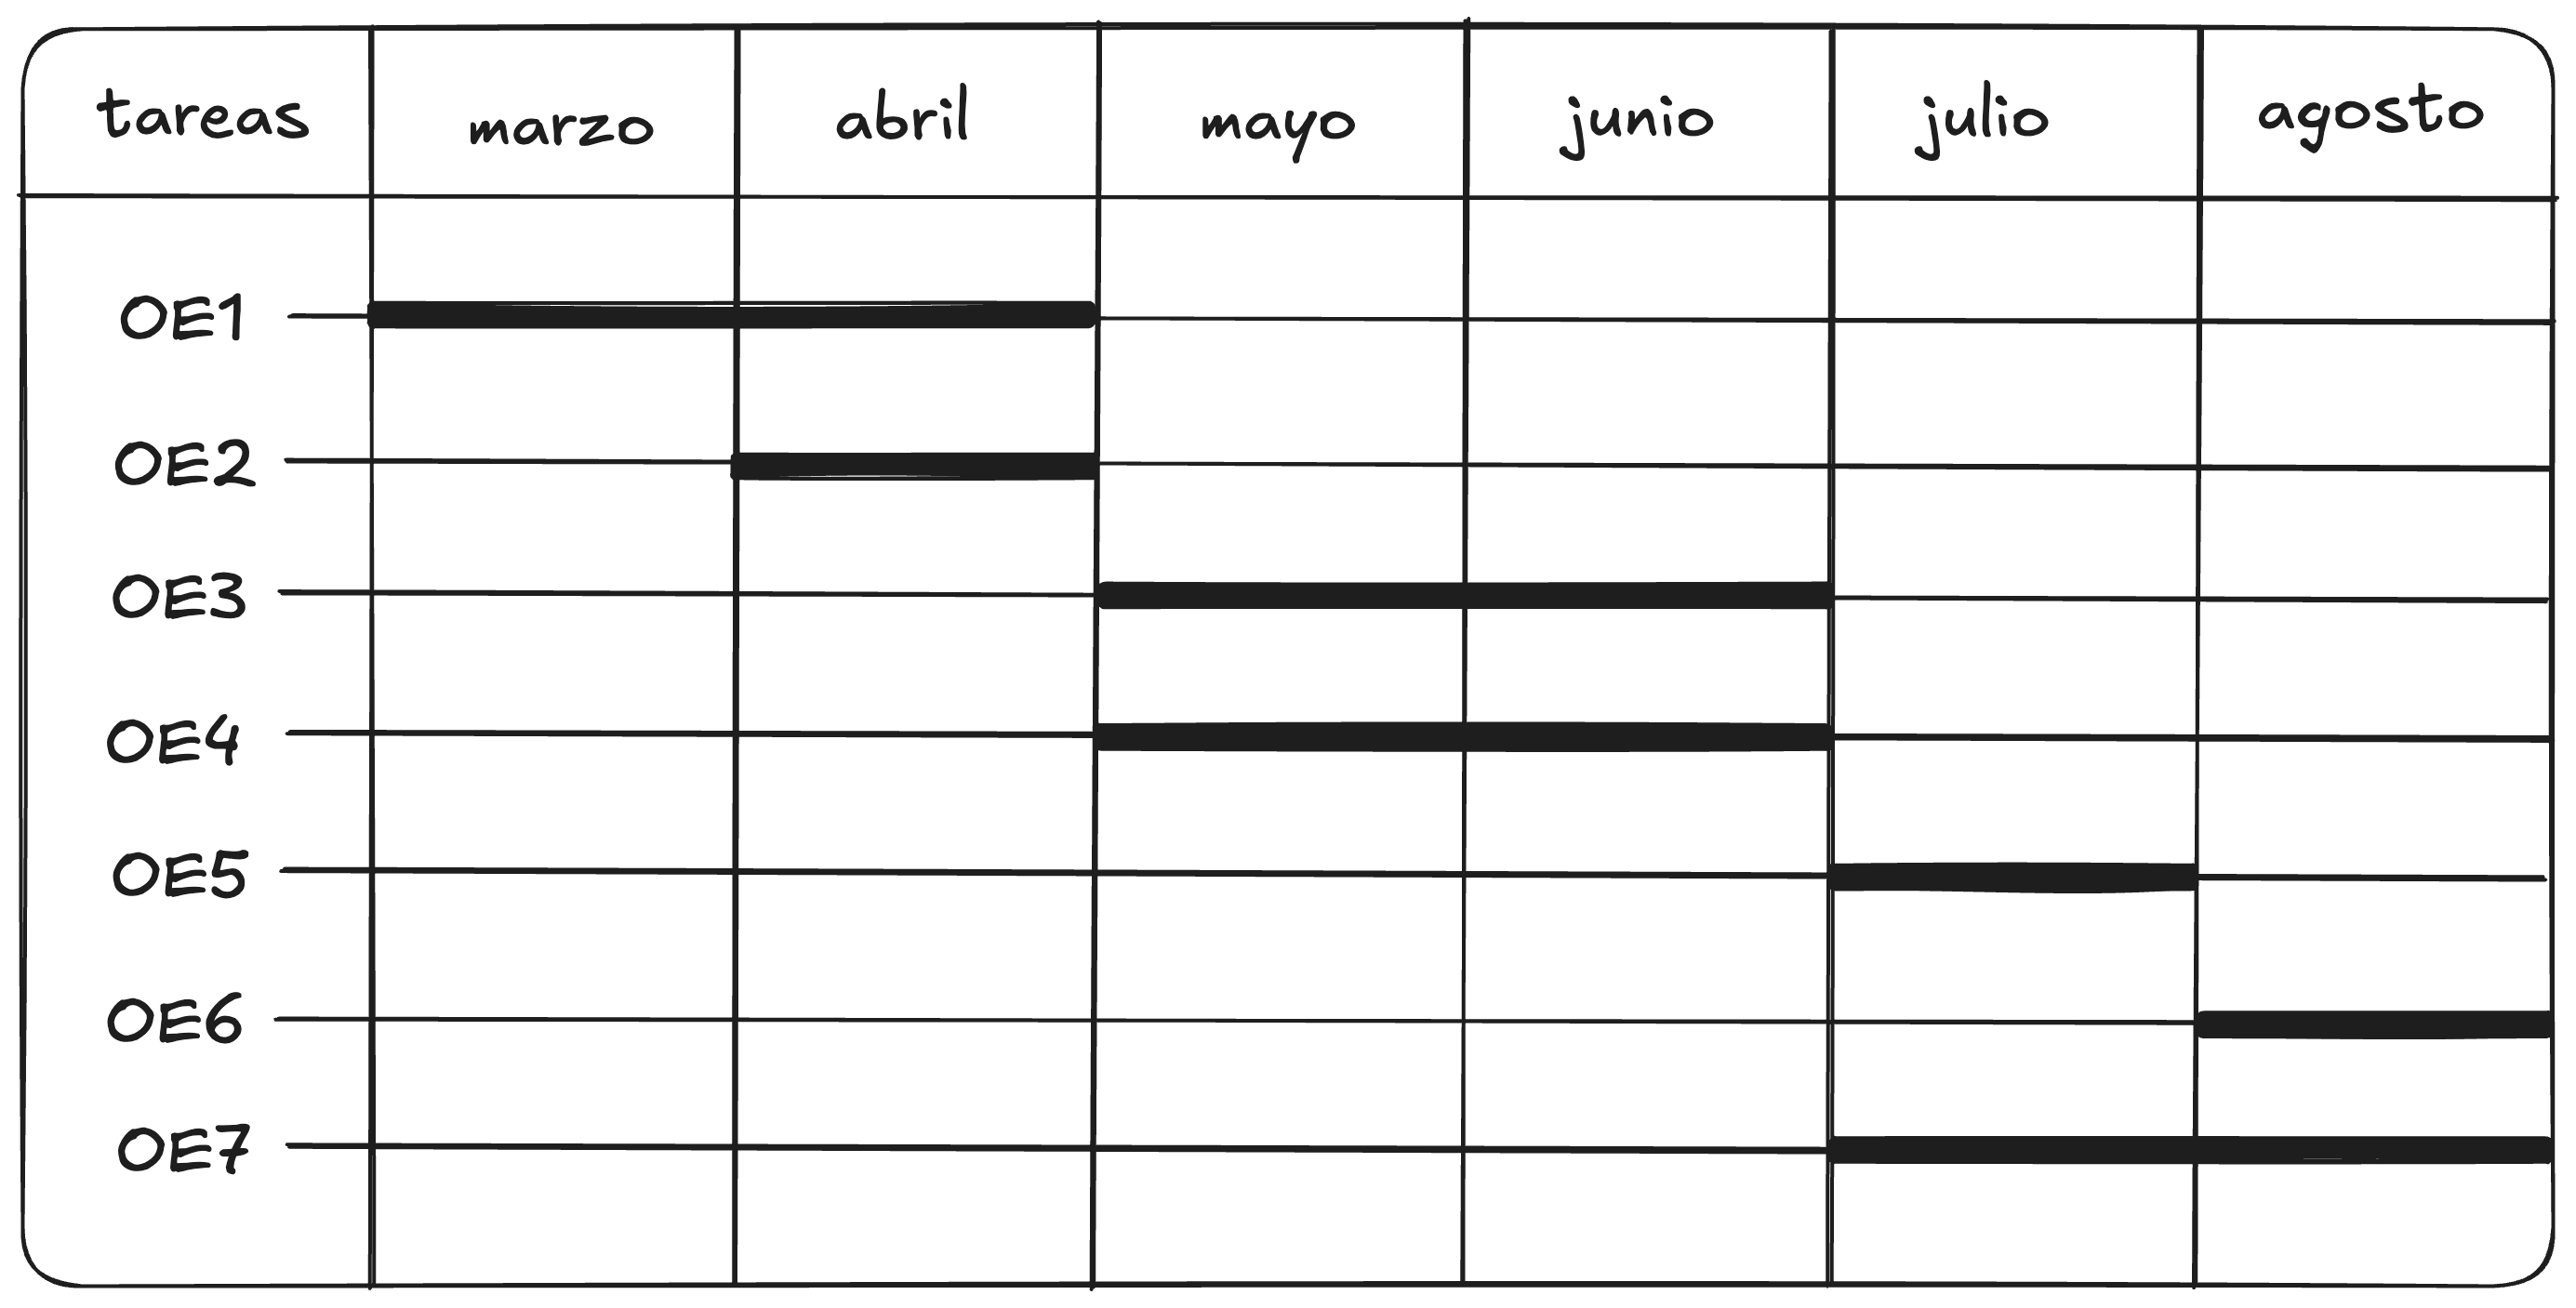
\includegraphics[width=\textwidth]{imagenes/gantt1.png}}
    %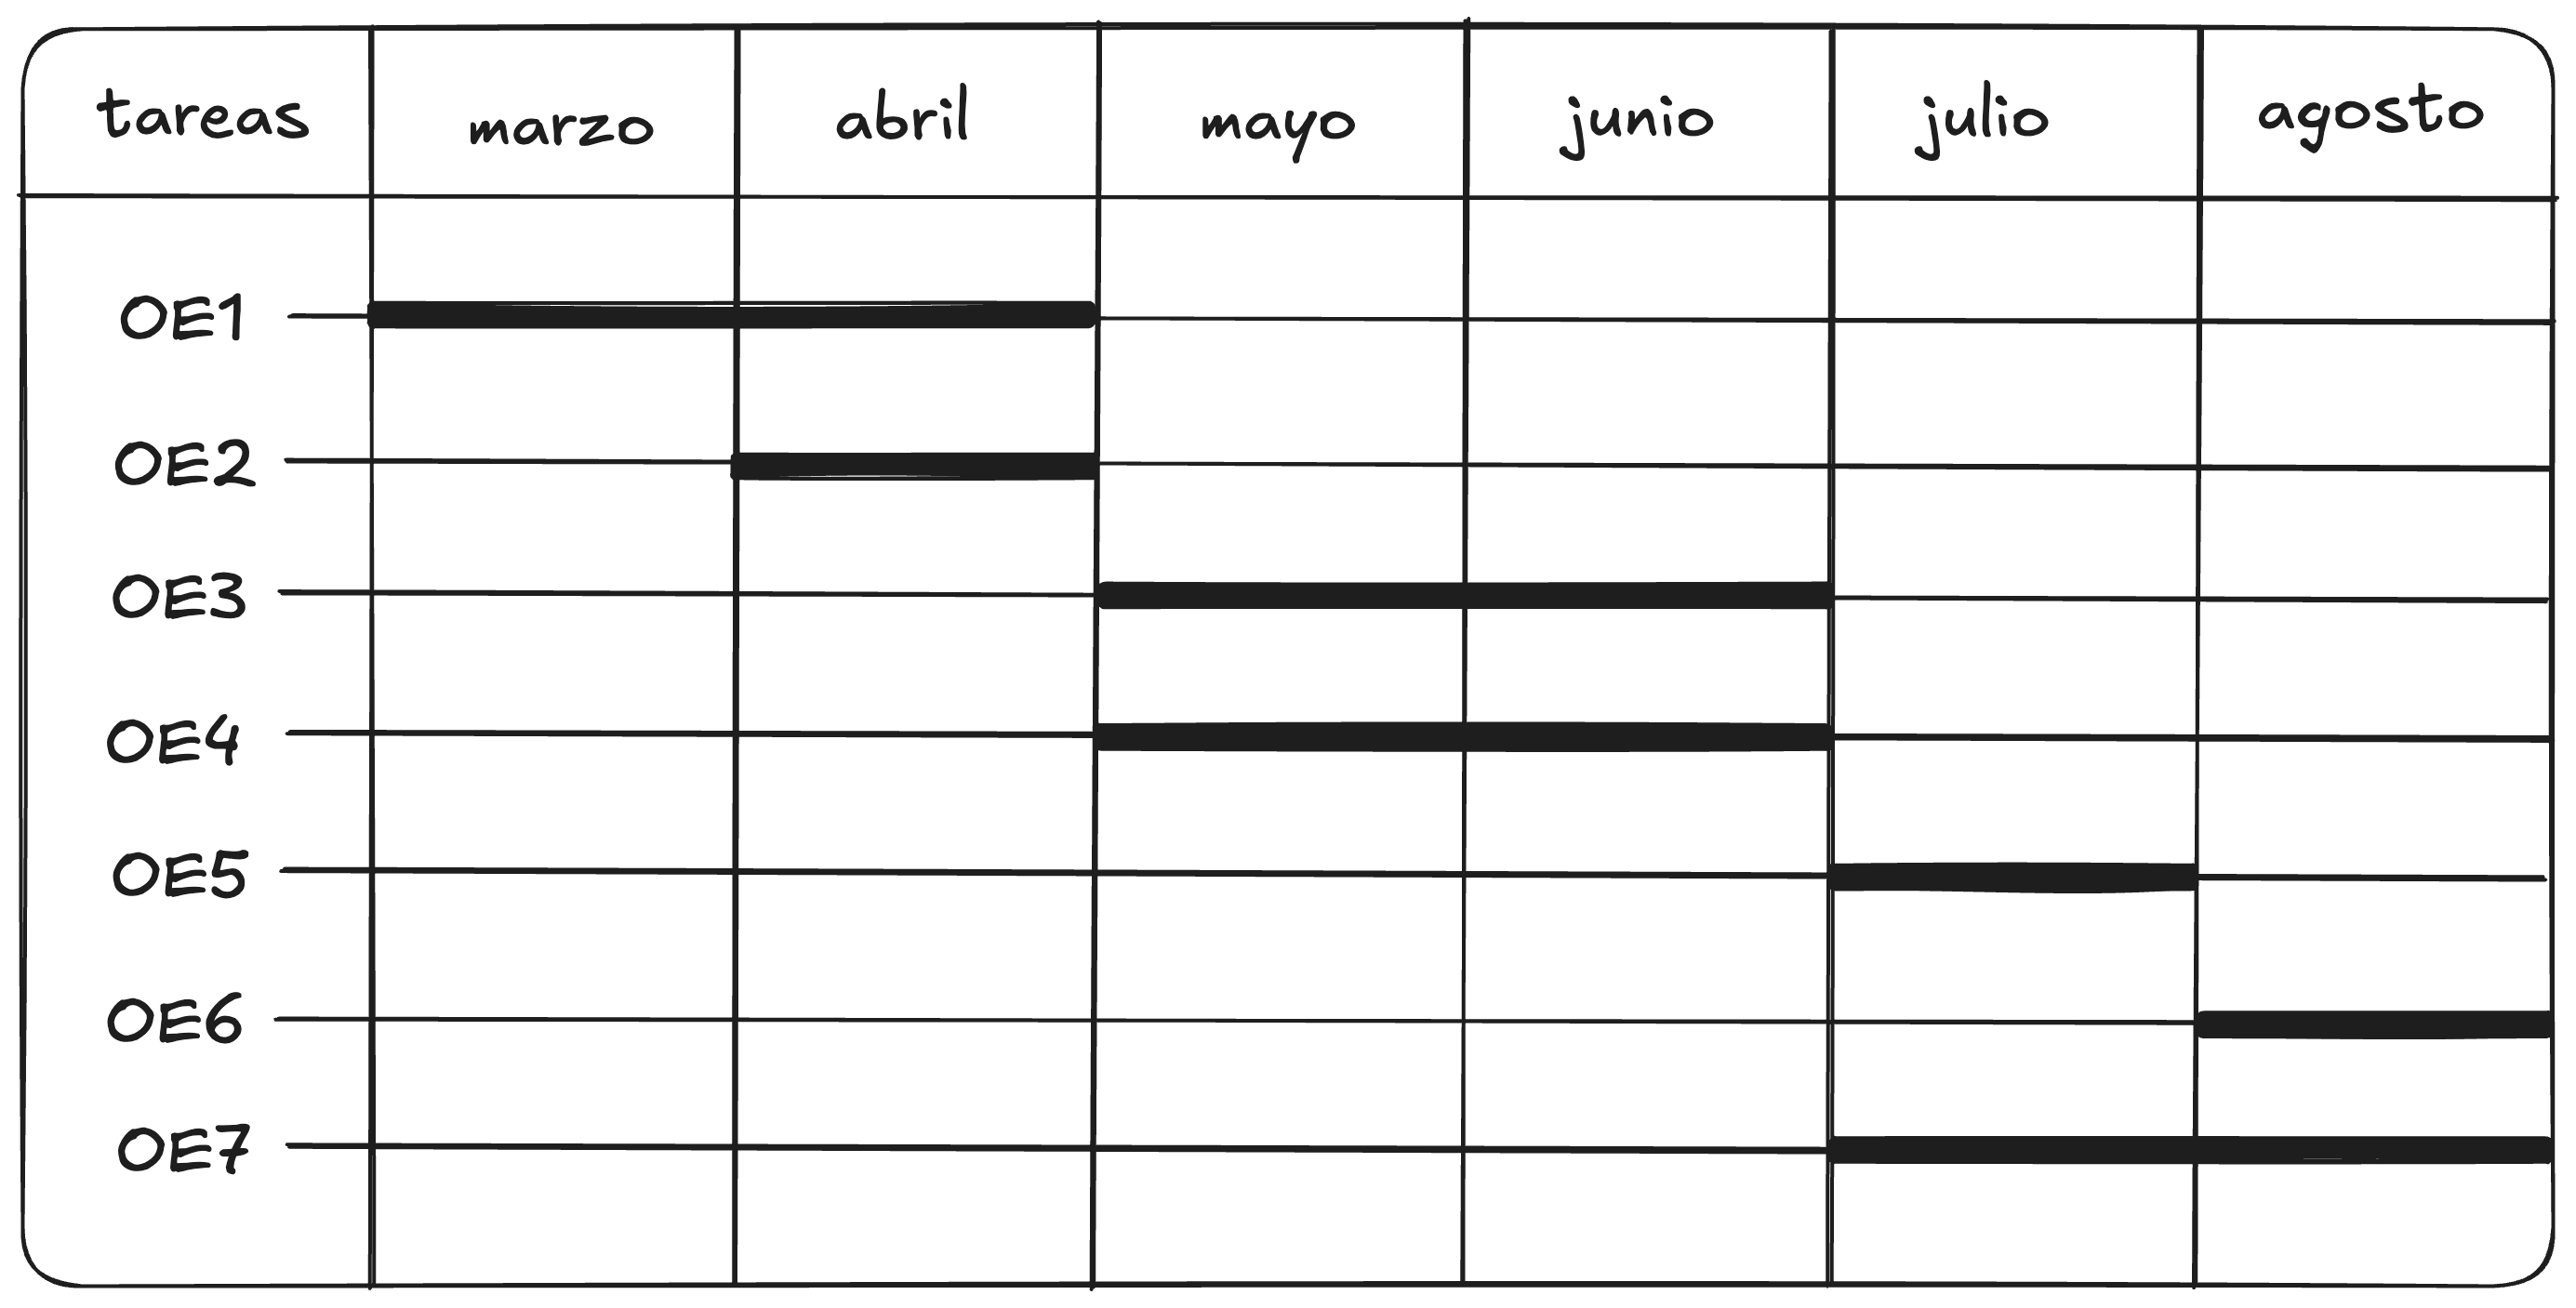
\includegraphics[width=\textwidth]{imagenes/gantt1.png}
    \caption{Diagrama de Gantt con la planificación del proyecto.}
\end{figure}

\section{Costes}

Si bien este proyecto tiene un enfoque académico, la elaboración de un presupuesto permite obtener una perspectiva más objetiva sobre el trabajo realizado. Este ejercicio aporta tanto un marco técnico como económico, acercando la iniciativa a escenarios reales y facilitando estimaciones útiles para futuras implementaciones o propuestas. Asimismo, contribuye a fundamentar las decisiones técnicas en función de su viabilidad financiera.

Para la estimación de costes, se han tenido en cuenta los recursos humanos, el equipamiento tecnológico y las herramientas de software empleadas. El cálculo se apoya en las tarifas promedio del sector de la programación en España y en los recursos técnicos requeridos. Los datos salariales se han extraído de la plataforma Glassdoor \cite{glassdoor}. Se ha considerado una duración total del proyecto de cinco meses.

\subsubsection{Costes humanos}

Para simular el coste de desarrollo de la plataforma en un entorno real, se ha considerado la contratación de un desarrollador junior a jornada completa (8 horas diarias, 21 días laborables al mes), lo que supone 168 horas mensuales. El salario anual medio para este perfil en España se estima en 20.000€.

\begin{equation*}
\text{Horas trabajadas al año} = 168\,\text{horas/mes} \times 12\,\text{meses} = 2.016\,\text{horas/año}
\end{equation*}

\begin{equation*}
\text{Coste por hora} = \frac{20.000\,€}{2.016\,\text{horas}} \approx 9,92\,€/hora
\end{equation*}

\begin{equation*}
\text{Coste mensual} = 9,92\,€/hora \times 168\,\text{horas} = 1.666,56\,€
\end{equation*}

\begin{equation*}
\text{Coste total (5 meses)} = 1.666,56\,€ \times 5 = 8.332,80\,€
\end{equation*}

\subsubsection{Costes de material}

Para el desarrollo del proyecto se han utilizado los siguientes equipos:

\begin{center}
\begin{tabular}{|l|c|}
\hline
\textbf{Material} & \textbf{Coste (€)} \\
\hline
Ordenador portátil & 2.000 \\
Servidor doméstico & 500 \\
\hline
\textbf{Total} & \textbf{2.500} \\
\hline
\end{tabular}
\end{center}

\subsubsection{Costes de herramientas}

Todo el software empleado en el desarrollo del proyecto corresponde a herramientas de licencia gratuita o planes gratuitos, por lo que no suponen coste adicional. No obstante, se ha utilizado la API de OpenAI con un coste total de 20€, además de un dominio personalizado con coste de 10€.

\begin{center}
\begin{tabular}{|l|c|}
\hline
\textbf{Herramienta} & \textbf{Coste (€)} \\
\hline
Software (licencias gratuitas) & 0 \\
Dominio & 10 \\
API OpenAI & 20 \\
\hline
\textbf{Total} & \textbf{30} \\
\hline
\end{tabular}
\end{center}

\subsubsection{Resumen de costes}

A continuación se muestra un resumen de todos los costes estimados para el proyecto:

\begin{center}
\begin{tabular}{|l|c|}
\hline
\textbf{Concepto} & \textbf{Coste (€)} \\
\hline
Coste de personal & 8.332,80 \\
Coste de material & 2.500 \\
Coste de herramientas & 30 \\
\hline
\textbf{Total} & \textbf{10.862,80} \\
\hline
\end{tabular}
\end{center}
\section{Estructura de la memoria}

El presente documento se estructura de la siguiente manera:

\begin{itemize}
    \item \textbf{Capítulo 1: Introducción}. Presenta el contexto, motivación, objetivos del proyecto, su planificación y costes, y finalmente la estructura del documento.
    
    \item \textbf{Capítulo 2: Estado del arte}. Revisión profunda de la literatura y trabajos previos.

    
    %\item \textbf{Capítulo 3: Diseño}. Descripción detallada de la arquitectura, modelos de datos y diseño de interfaces de la aplicación.
    
    \item \textbf{Capítulo 3: Implementación}. Explicación del proceso de desarrollo de la aplicación, incluyendo tecnologías utilizadas, configuración del entorno y aspectos técnicos relevantes.
    
    %\item \textbf{Capítulo 5: Resultados y evaluación}. Presentación de los resultados obtenidos y evaluación del desempeño de la aplicación en términos de usabilidad, eficiencia y utilidad.
    
    \item \textbf{Capítulo ?: Conclusiones y trabajo futuro}. Resumen de las contribuciones del proyecto, limitaciones encontradas y posibles líneas de trabajo futuro.
\end{itemize}


\chapter{Estado del arte}

Este capítulo ofrece una visión actualizada de los recursos, tecnologías y enfoques más relevantes para la gestión y análisis de datos clínicos. Se abordan las principales bases de datos abiertas, los modelos de almacenamiento y consulta, las arquitecturas de software más empleadas, las herramientas de visualización y el impacto de la Inteligencia Artificial en el ámbito sanitario, situando el proyecto dentro del contexto de la innovación digital en salud.

%\section{El Movimiento hacia la Ciencia Abierta en la Investigación Médica}
\section{Ciencia abierta y bases de datos clínicas}

En las últimas décadas se ha consolidado un movimiento hacia los datos clínicos abiertos, promoviendo la disponibilidad de bases de datos sanitarias para la comunidad investigadora. La idea de ciencia abierta sostiene que la libre disponibilidad de datos y códigos favorece la transparencia, la reproducibilidad y la colaboración en la investigación biomédica \cite{Lvovs2025_balancing}. Sin embargo, históricamente los datos clínicos han estado protegidos en archivos hospitalarios, difíciles de acceder por razones legales, éticas y técnicas. En respuesta, iniciativas académicas y gubernamentales han impulsado la creación de conjuntos de datos clínicos de acceso abierto, debidamente anonimizados, que permiten a investigadores de todo el mundo analizar información real de pacientes sin vulnerar la privacidad. Estos recursos han transformado la investigación médica al reducir barreras de acceso y fomentar prácticas reproducibles en análisis de datos sanitarios

\newpage
Los datos clínicos se pueden clasificar en cuatro grandes modalidades complementarias:


(i) \emph{Señales fisiológicas de alta frecuencia.} Series temporales de ECG, presión arterial invasiva, fotopletismografía o EEG. Podemos destacar la clásica MIT-BIH Arrhythmia Database (1980), patrón de referencia para algoritmos de ECG \cite{Impact_MIT-BIH}; el MIMIC Waveform Database, que enlaza miles de horas de señales con los datos clínicos de MIMIC \cite{Moody2022_MIMICIVWaveform}; y HiRID, con 712 variables registradas cada dos minutos en más de 30 000 estancias UCI \cite{Faltys2021HiRID}.

(ii) \emph{Imágenes médicas con anotaciones diagnósticas.}  Abarcan radiografías, TC, RM, PET e incluso histopatología digital, cada una acompañada de etiquetas o informes de hallazgo.  Las bases más usadas en radiología son ChestXray14 y CheXpert, ambas con cientos de miles de radiografías torácicas etiquetadas para patologías pulmonares \cite{irvin2019chexpertlargechestradiograph}, y MIMIC-CXR por parte de la familia MIMIC \cite{Johnson2019_MIMICCXR}.  En oncología destacan las colecciones TCGA/TCIA \cite{TCGA,Clark2013_TCIA}, y en neuroimagen la iniciativa ADNI \cite{Petersen2010_ADNI}.  Estos recursos posibilitan evaluar modelos de visión computacional con criterios homogéneos.

(iii) \emph{Texto clínico desidentificado.}  Incluye notas de evolución, informes radiológicos, resúmenes de alta, entre otros.  Representa alrededor del 80 \% de la información clínica, pero su liberación es más compleja por contener PHI (Protected Health Information).  Los desafíos i2b2/n2c2, pioneros al proveer corpora anonimizados, constituyen la plataforma estándar para comparar sistemas de procesamiento del lenguaje natural médico \cite{n2c2}.  El ecosistema MIMIC también complementa este dominio con millones de notas clínicas \cite{Johnson2023_MIMICIVNote}. 

(iv) \emph{Datos estructurados de historias clínicas electrónicas (EHR).}  Comprenden tablas con demografía, diagnósticos (ICD-9/10), procedimientos, resultados de laboratorio, medicación y constantes vitales.  Son la base de estudios epidemiológicos y de la construcción de modelos pronósticos.  Entre los conjuntos abiertos más influyentes figuran NHANES \cite{NHANES}, UK Biobank \cite{Sudlow2015_UKBiobank}, eICU \cite{Pollard2018} y, sobre todo, la serie MIMIC en la que se enfoca este trabajo.

Desde 1999 PhysioNet \cite{PhysioNet_paper} estableció un marco seguro y reproducible para compartir todo tipo de registros hospitalarios.  Bajo ese paraguas nació el ecosistema MIMIC: la primera versión (1996) contenía 90 pacientes UCI \cite{Moody1996_MIMIC}; MIMIC-II (2011) multiplicó tamaño y variables al extraer directamente de los sistemas clínicos \cite{Saeed2011_MIMICII}; MIMIC-III (2015) superó los 40 000 pacientes y se convirtió en la referencia mundial \cite{MIMICIII_paper}; MIMIC-IV \cite{MIMICIV_paper} amplía y moderniza el conjunto.  Esta trayectoria demuestra cómo los EHR han pasado a ser un recurso científico global, permitiendo investigar la fisiopatología crítica con una profundidad antes impensable.

\begin{figure}[ht]
    \centering
    \fbox{
\includegraphics[width=0.4\textwidth]{imagenes/physionet-logo.png}}
    %
\includegraphics[width=0.4\textwidth]{imagenes/physionet-logo.png}
    \caption{Logo de PhysioNet.}
\end{figure}

\newpage
En conjunto, el panorama de datos clínicos abiertos ofrece múltiples alternativas, pero MIMIC-IV destaca como la más idónea para este trabajo: combina un gran volumen de datos reciente, buena documentación, y módulos complementarios. Sobre esta base, el proyecto diseñará una plataforma que haga de este conjunto de datos una fuente accesible de conocimiento, alineada con los principios de ciencia abierta.


%\section{Tecnologías para la Gestión y Almacenamiento de Datos Sanitarios}
\section{Tecnologías de Gestión y Almacenamiento de Datos Sanitarios}




En el plano tecnológico, la forma de almacenar y consultar la información marca las posibilidades reales de análisis. De forma general, los sistemas de gestión de bases de datos se dividen en dos grandes familias: relacionales y no relacionales. Las del primer grupo organizan la información en tablas de filas y columnas conectadas por claves y se consultan con SQL, siendo las más usadas MySQL, PostgreSQL, Oracle y SQL Server.  Las no relacionales, llamadas NoSQL, almacenan los datos como documentos, pares clave-valor, columnas o grafos y permiten esquemas flexibles y escalado horizontal; las más populares son MongoDB y Couchbase en la categoría de documentos, Cassandra en column-family, Redis en clave-valor y Neo4j en grafos \cite{DBEngines2025}.

\begin{figure}[H]
    \centering
    \fbox{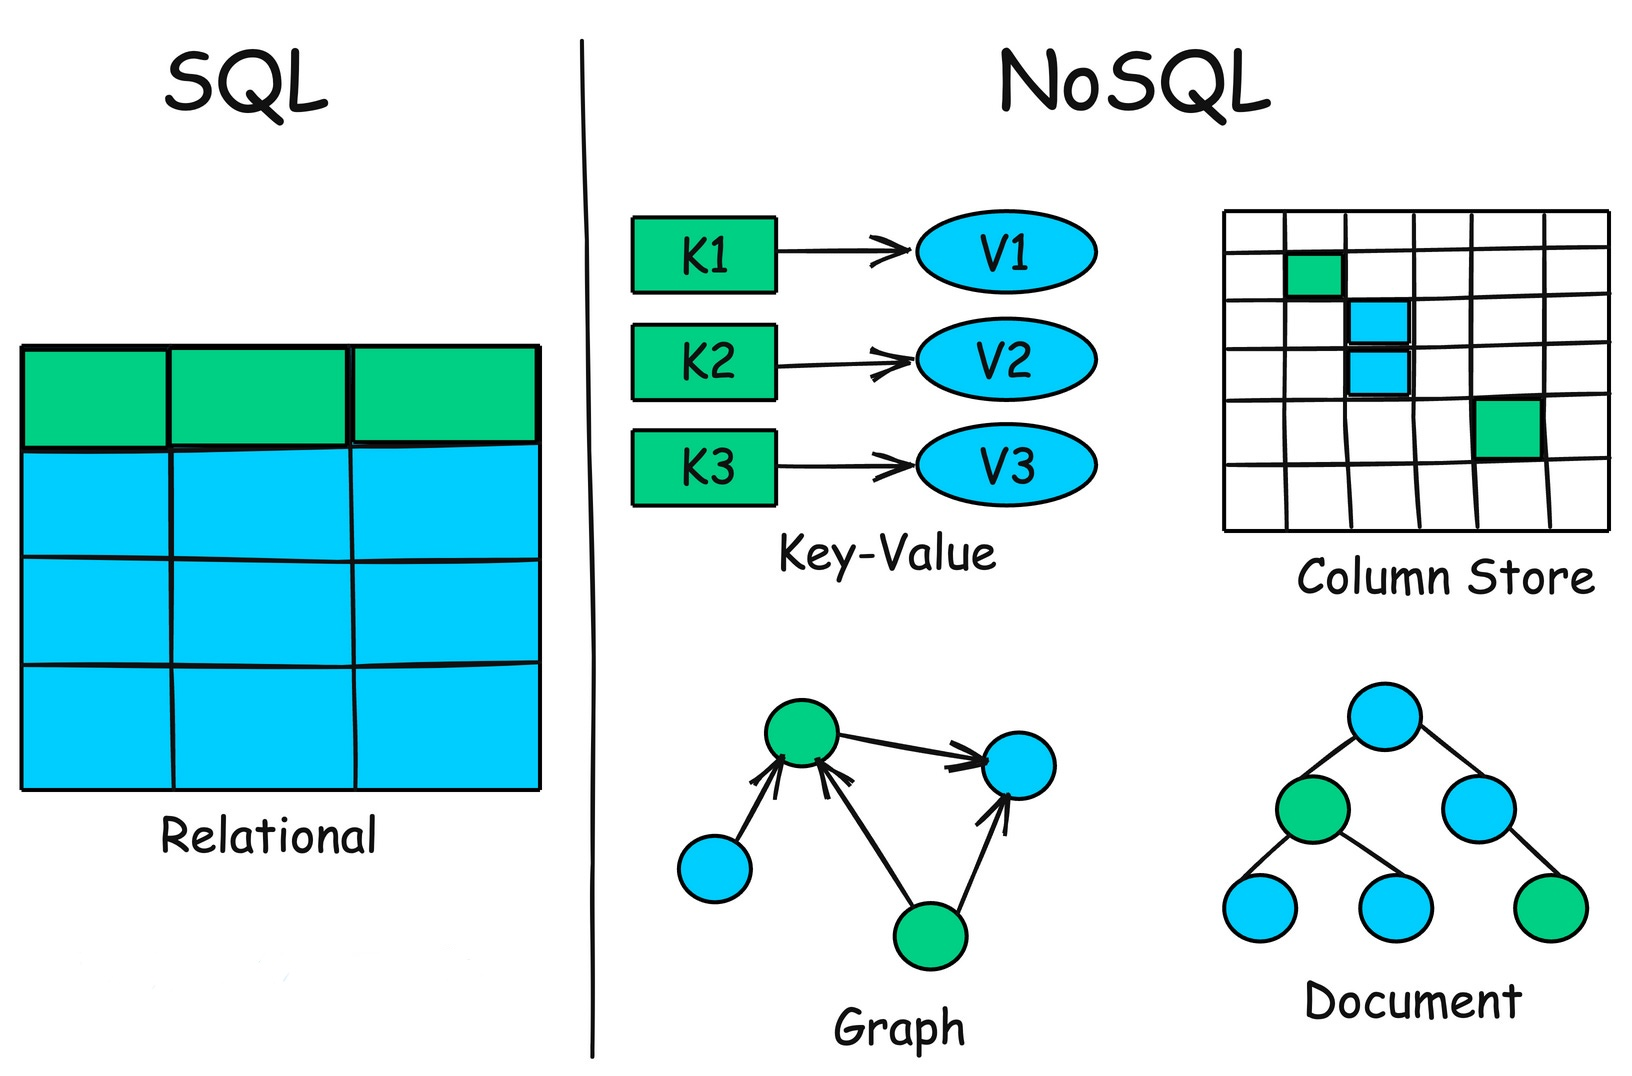
\includegraphics[width=0.75\textwidth]{imagenes/sqlvsnosql.jpg}}
    %
\includegraphics[width=0.4\textwidth]{imagenes/physionet-logo.png}
    \caption{SQL vs NoSQL \cite{sqlvsnosqlfoto}.}
\end{figure}


En el ámbito sanitario la mayoría de los sistemas de historia clínica electrónica se ha construido sobre gestores relacionales porque los registros se modelan de forma natural en tablas normalizadas y el lenguaje SQL facilita auditoría y trazabilidad.  Sin embargo, los hospitales también generan notas de texto libre, señales continuas, imágenes y estructuras jerárquicas; ello ha impulsado el uso de bases documentales y de grafos, que aceptan datos heterogéneos y simplifican la ingesta sin migraciones de esquema cada vez que aparece un nuevo campo \cite{GAMAL2021103670,MongoFHIR}.

%A pesar de que MIMIC-IV se distribuye en un esquema relacional, para este proyecto cargaremos el conjunto en MongoDB. Este modelo documental nos permite agrupar los datos que se deseen en un único documento anidado, elimina la necesidad de combinar una veintena de tablas con uniones complejas y responde con menor latencia a las búsquedas interactivas que planteará el usuario desde la interfaz web.  Además, nos ofrece flexibilidad y escalabilidad si en el futuro se desea incorporar señales o imágenes, de modo que se adapta mejor a la naturaleza exploratoria y multimodal de nuestra aplicación.


%\section{Arquitecturas de Software y el Stack Tecnológico Web}
\section{Arquitecturas de Software y  Stack Web}

La evolución del desarrollo de software ha experimentado una transformación radical desde las aplicaciones de escritorio tradicionales hacia ecosistemas web distribuidos. En los años 90, la Web se caracterizaba por páginas estáticas servidas directamente desde servidores, pero la creciente demanda de interactividad y funcionalidad dinámica impulsó el desarrollo de tecnologías como CGI, PHP y posteriormente frameworks más sofisticados \cite{Ritesh2023_WebEvolution}. Esta evolución culminó en las aplicaciones web contemporáneas, que se fundamentan en la arquitectura cliente-servidor, donde el frontend ejecutado en el navegador del usuario se comunica con un backend que procesa la lógica y gestiona el acceso a los datos \cite{Nyabuto2024_ClientServer}. Esta separación de responsabilidades permite que cada componente evolucione independientemente, facilita el mantenimiento del código y posibilita la escalabilidad según las necesidades específicas de cada capa. En el contexto de aplicaciones de análisis de datos como la que nos ocupa, esta arquitectura resulta especialmente ventajosa al permitir que el procesamiento computacionalmente intensivo se realice en el servidor mientras el cliente se centra en la presentación interactiva de los resultados.

%begin{figure}[H]
%    \centering
%    \fbox{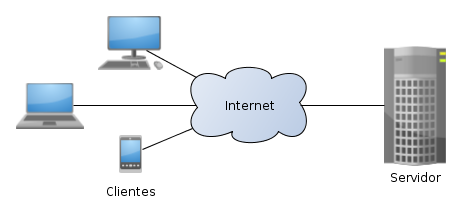
\includegraphics[width=0.75\textwidth]{imagenes/Cliente-Servidor.png}}
%    %
\includegraphics[width=0.4\textwidth]{imagenes/physionet-logo.png}
%    \caption{Diagrama cliente-servidor \cite{clienteservidorfoto}.}
%\end{figure}

\begin{figure}[H]
    \centering
    \fbox{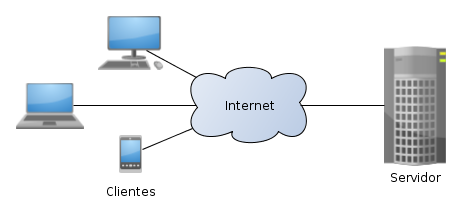
\includegraphics[width=0.85\textwidth]{imagenes/Cliente-Servidor.png}}
    %
\includegraphics[width=0.4\textwidth]{imagenes/physionet-logo.png}
    \caption{Diagrama cliente-servidor \cite{clienteservidorfoto}.}
\end{figure}




En cuanto a las tecnologías de servidor, existe un amplio abanico de alternativas consolidadas, cada una con fortalezas específicas según el contexto de aplicación. Node.js con frameworks como Express o Fastify permite utilizar JavaScript en el servidor, facilitando el desarrollo full-stack y ofreciendo excelente rendimiento para aplicaciones I/O intensivas. Python, con opciones como Django, Flask y FastAPI, destaca en proyectos que requieren análisis de datos o integración con librerías científicas \cite{Castro2023_PythonDataScience}. Java con Spring Boot sigue siendo una opción robusta para aplicaciones empresariales de gran escala, mientras que lenguajes como Go y Rust están ganando adopción por su rendimiento superior en sistemas distribuidos. %En el contexto de este proyecto, donde el procesamiento de datos biomédicos y la futura integración de modelos de inteligencia artificial son requisitos centrales, se ha optado por FastAPI con Python, aprovechando tanto su ecosistema maduro para análisis de datos como su capacidad para generar APIs modernas y eficientes.

Por otro lado, las tecnologías frontend han experimentado una evolución significativa desde las aplicaciones de página única (SPA) hacia enfoques más sofisticados que combinan diferentes estrategias de renderizado. Los frameworks principales \cite{Swacha2023_WebFrameworks} incluyen React, que ofrece un ecosistema maduro y flexible basado en componentes; Vue.js, conocido por su curva de aprendizaje suave y documentación excelente; y Angular, que proporciona un framework completo con opiniones definidas para aplicaciones empresariales. Paralelamente, han surgido meta-frameworks como Next.js, Nuxt.js y SvelteKit que extienden estos frameworks base con capacidades de renderizado del lado del servidor (SSR), generación de sitios estáticos (SSG) y optimizaciones automáticas. %Para este proyecto se ha seleccionado Next.js sobre React, desplegado en Vercel, una combinación que permite aprovechar tanto el renderizado híbrido para optimizar el rendimiento del análisis y visualización de datos.

\begin{figure}[H]
\centering
\fbox{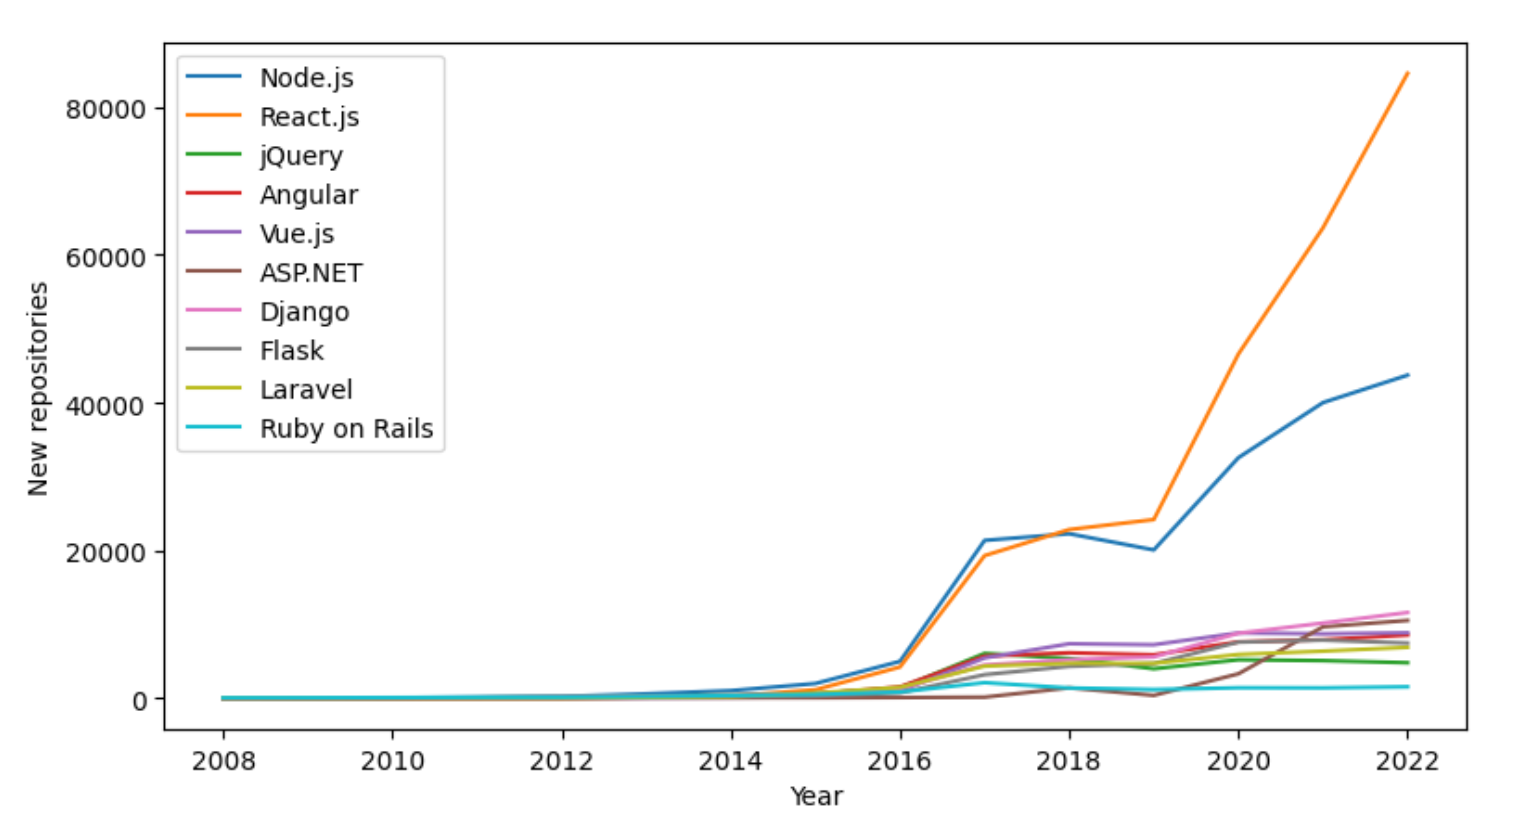
\includegraphics[width=1\textwidth]{imagenes/grafica_frameworks.png}}
%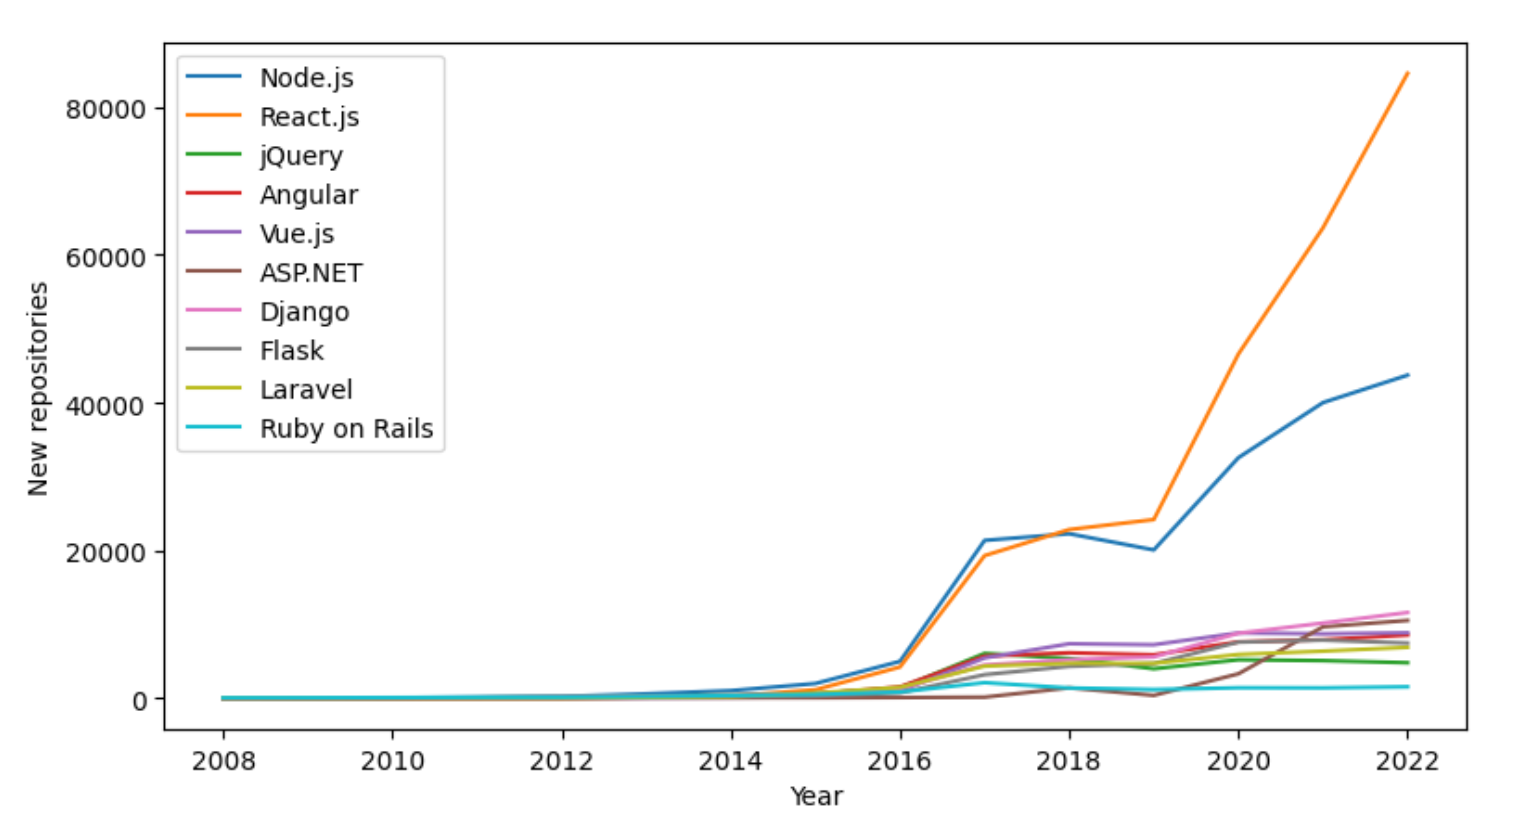
\includegraphics[width=\textwidth]{imagenes/grafica_frameworks.png}
\caption{Evolución de la popularidad de frameworks web según el número de repositorios creados anualmente en GitHub \cite{Swacha2023_WebFrameworks}.}
\label{fig:frameworks_github}
\end{figure}



%\section{Herramientas y Técnicas de Visualización Interactiva de Datos}
\section{Herramientas de Visualización Interactiva de Datos}

Para la visualización de datos en aplicaciones web existen principalmente dos tipos de herramientas: plataformas de business intelligence (Tableau, Power BI, Metabase) y librerías de programación para desarrolladores. Las plataformas de business intelligence permiten a usuarios no técnicos explorar y analizar datos mediante interfaces gráficas intuitivas, facilitando la creación de dashboards interactivos y la generación de informes sin necesidad de programar. Sin embargo, estas plataformas suelen estar más orientadas al análisis empresarial general y pueden presentar limitaciones cuando se requiere una personalización avanzada o la integración directa con aplicaciones web personalizadas.

Por otro lado, las librerías de programación ofrecen a los desarrolladores un control total sobre la visualización y permiten crear gráficos completamente adaptados a las necesidades de cada proyecto. Entre las librerías más utilizadas para Javascript destacan D3, Chart.js, Plotly.js y ECharts, por nombrar algunas, aunque el ecosistema es muy amplio y en constante evolución \cite{Monterail2024_JSViz}. Estas herramientas permiten desde la creación de gráficos básicos hasta visualizaciones interactivas complejas, integrándose perfectamente en aplicaciones web modernas y proporcionando una experiencia de usuario más dinámica y personalizada.


%En el contexto de este proyecto, se ha optado por usar dos librerías distintas, dependiendo de la complejidad del gráfico, pero que son desarrolladas por la misma compañía denominada Observable \cite{observable}. Se utiliza D3 \cite{d3} para visualizaciones altamente personalizadas que requieren máximo control granular sobre cada elemento gráfico, lo que resulta especialmente útil para representar datos clínicos complejos o relaciones no convencionales. Por otro lado, se reserva Plot \cite{observableplot} para las visualizaciones más sencillas y habituales, aprovechando sus soluciones preestablecidas que aceleran el desarrollo y reducen la carga de trabajo en la implementación. Esta combinación permite mantener un enfoque progresivo en complejidad, acelerando la rapidez de implementación y manteniendo una coherencia estética y técnica al permanecer dentro del mismo ecosistema de herramientas.

\begin{figure}[H]
    \centering    \fbox{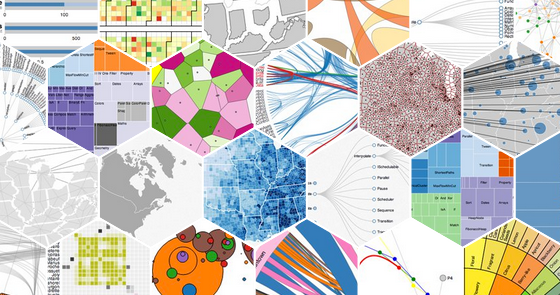
\includegraphics[width=0.85\textwidth]{imagenes/d3.png}}
    %
\includegraphics[width=0.4\textwidth]{imagenes/physionet-logo.png}
    \caption{Visualizaciones realizadas con D3 \cite{d3foto}.}
\end{figure}



%\section{Aplicaciones de Inteligencia Artificial en el Análisis Clínico}
\section{Grandes Modelos de Lenguaje (LLM) en Medicina}

Los grandes modelos de lenguaje basados en Transformers han irrumpido en la práctica clínica porque ofrecen comprensión contextual y generación de texto con una fluidez cercana a la humana. A diferencia de los modelos supervisados tradicionales, los LLMs aprenden a partir de preentrenamiento masivo y pueden adaptarse con pocos ejemplos, rasgo que resulta valioso cuando los conjuntos de datos clínicos etiquetados son escasos. Este cambio de paradigma coincide con la disponibilidad de texto sanitario desidentificado, lo que ha catalizado su adopción en investigación biomédica.


Después de la aparición de modelos generalistas como GPT-3 \cite{Brown2020GPT3} se publicaron variantes especializadas en biomedicina entrenadas sobre literatura científica y notas de pacientes. ClinicalBERT \cite{Boag2020_ClinicalBERT} y BioGPT \cite{Lee2020_BioBERT} demostraron que un preentrenamiento adicional en dominio mejora la extracción de entidades médicas y la clasificación de relaciones. Más recientemente, GatorTron \cite{Yang2022_GatorTron}, Med-PaLM 2 \cite{Singhal2023_MedPaLM2} y Llama-Med \cite{Xie2024_MeLLaMA} ampliaron el tamaño de parámetros y el repertorio de instrucciones clínicas, acercándose al rendimiento de especialistas humanos en tareas de respuesta a preguntas complejas.

La integración de estos modelos en sistemas hospitalarios adopta varias estrategias. La más extendida es la generación aumentada por recuperación, en la que el LLM consulta primero una base indexada de guías clínicas o registros electrónicos y después compone la respuesta citando la información recuperada \cite{RAGSurvey2023}. Otra línea es el ajuste fino con instrucciones específicas que enseñan al modelo a traducir preguntas en lenguaje natural a consultas estructuradas sobre bases de datos; ChatEHR es un ejemplo que opera sobre historiales electrónicos \cite{Stanford2025_ChatEHR}. El Model Context Protocol (MCP) propone una capa intermedia para que el modelo invoque herramientas, agentes o bases de datos de forma segura, lo que facilita operaciones más complejas que la simple generación de texto \cite{AnthropicMCP2024}.

El éxito de estas técnicas depende de corpus clínicos abiertos que permitan la adaptación en dominio. Las notas de MIMIC-III y MIMIC-IV \cite{Johnson2023_MIMICIVNote}, los desafíos i2b2/n2c2 \cite{n2c2} (ya mencionadas anteriormente) y colecciones de pregunta–respuesta como PubMedQA \cite{Jin2019_PubMedQA} y MedQA \cite{Jin2020_MedQA} constituyen hoy los pilares para la evaluación reproducible de PLN médico. No obstante, la sensibilidad de la información obliga a procesos de anonimización rigurosos y a la aplicación de licencias restrictivas.

A pesar de su potencial, los LLMs plantean riesgos significativos. Pueden generar afirmaciones verosímiles pero erróneas, lo que compromete la seguridad clínica; además, arrastran sesgos demográficos si los datos de entrenamiento son incompletos y pueden filtrar información protegida si no se controla el \textit{fine-tuning}. La comunidad trabaja en métricas de evaluación específicas y en detectores de alucinaciones, pero todavía no existe un consenso regulatorio sobre su despliegue en entornos asistenciales \cite{Bommasani2022_FoundationModels}. Estos retos marcan la agenda de investigación actual y condicionan las directrices éticas para cualquier sistema que integre LLMs con datos reales de pacientes.



\section{Aplicaciones existentes similares}\

En el ámbito hospitalario existen numerosas soluciones comerciales consolidadas para la gestión y análisis de datos clínicos. Sistemas como Epic Systems integran módulos de visualización de indicadores, generación de informes y cuadros de mando en tiempo real, con funcionalidades que incluyen predicción de riesgos, alertas clínicas y exploración de cohortes directamente sobre la historia clínica electrónica \cite{Epic}. Este tipo de plataformas están diseñadas para su uso en entornos de producción con pacientes reales y representan el estándar en hospitales de gran escala, aunque se trata de soluciones cerradas y de acceso restringido al entorno clínico que las contrata.

En contraste, las opciones de código abierto para la visualización de datos médicos son mucho más limitadas en número y funcionalidades. LinkR es un proyecto reciente orientado a la exploración y visualización de datos clínicos siguiendo el estándar OMOP \cite{linkR}. Como otro ejemplo, Metriport a pesar de no ser su función principal, permite visualizar los datos clínicos, usando IA para resumir los historiales clínicos de los pacientes, y también posee una capa open source \cite{metriport}. En general, se ha encontrado que son muy escasos los recursos abiertos, actualizados y en mantenimiento en este ambito.


En cuanto a la exploración específica de MIMIC-IV, no se han identificado plataformas web abiertas que ofrezcan de forma nativa una visualización interactiva del conjunto de datos. La aproximación más utilizada en la literatura consiste en cargar el conjunto de datos en entornos analíticos en la nube, como Google BigQuery combinado con Looker Studio, lo que permite construir paneles y gráficos sin necesidad de programación \cite{bigquery_mimic}. Otra alternativa es la conversión de los datos al estándar OMOP, lo que hace posible su explotación a través de herramientas como OHDSI Atlas, que incluye funcionalidades de análisis de cohortes y visualización \cite{OHDSI_Atlas, MIMICIV_OMOP_Demo}. No obstante, estas opciones requieren configuraciones avanzadas y no existen soluciones abiertas, listas para usar, que faciliten directamente la exploración gráfica de MIMIC-IV a investigadores sin conocimientos técnicos.



\section{Síntesis y foco del presente TFG}

El repaso realizado muestra un contraste evidente entre las soluciones comerciales y el panorama abierto. En el entorno hospitalario, las grandes plataformas de EHR concentran el grueso de la innovación en visualización y análisis de datos clínicos. Se trata de sistemas completos, diseñados para la práctica asistencial diaria, con interfaces pulidas y funcionalidades avanzadas de predicción y apoyo a la decisión clínica. Sin embargo, son soluciones cerradas y restringidas a los centros que las contratan.

En el ámbito open source, la situación es distinta. Existen numerosas bases de datos abiertas que han impulsado la investigación biomédica en todo el mundo. Sin embargo, las herramientas disponibles para explorarlas son menos accesibles para usuarios sin experiencia técnica. Los investigadores suelen recurrir a consultas SQL, entornos estadísticos o integraciones complejas con plataformas de terceros, lo que limita su aprovechamiento por parte de perfiles clínicos sin formación tecnológica. Las interfaces gráficas abiertas y mantenidas son escasas y, cuando existen, tienden a estar más orientadas a la investigación metodológica que a la usabilidad clínica.

En este contexto se sitúa el presente trabajo. El objetivo no es competir con los sistemas hospitalarios consolidados, sino plantear un prototipo que sirva como demostración de cómo un conjunto de datos abierto como MIMIC-IV puede hacerse accesible mediante una plataforma web sencilla de usar. El sistema combina visualización interactiva con integración de modelos de inteligencia artificial recientes, ilustrando cómo los profesionales sin conocimientos técnicos podrían extraer valor de bases de datos clínicas abiertas. De este modo, el proyecto se posiciona como un puente entre la abundancia de datos disponibles y la carencia de interfaces accesibles para su exploración.



\chapter{Análisis y especificación de requisitos}

En este capitulo se trata de comprender y definir las necesidades, objetivos, funcionalidades y actores que van a hacer uso de la herramienta a desarrollar. Para lograrlo se van plantear diferentes requisitos funcionales, no funcionales y casos de uso como solución a las siguientes preguntas.

- ¿Cómo debe comportarse la aplicación?

- ¿Qué flujo tiene cada funcionalidad?

- ¿Qué limitaciones y restricciones existen?

- ¿Qué tipos de usuarios existen?

- ¿Qué acciones puede realizar cada tipo de usuario?

- ¿Cómo satisfacer las necesidades del 
usuario?

- ¿Qué espera el usuario?


%\begin{itemize}
%    \item ¿Cómo debe comportarse la aplicación?
%    \item ¿Qué flujo tiene cada funcionalidad?
%    \item ¿Qué limitaciones y restricciones existen?
%    \item ¿Qué tipos de usuarios existen?
%    \item ¿Qué acciones puede realizar cada tipo de usuario?
%    \item ¿Cómo satisfacer las necesidades del usuario?
%    \item ¿Qué espera el usuario?
%\end{itemize}


\section{Especificación de requisitos}

\subsection{Requisitos funcionales}

Los requisitos funcionales (R.F.) son aquellos que definen como un sistema o componente tiene que funcionar o comportarse. Estos en este caso,
son los siguientes:

\begin{itemize}
    \item R.F. 1: El sistema permitirá representar información a través de distintas visualizaciones.
    \item R.F. 2: Las visualizaciones serán interactivas cuando el usuario hace click o hover.
    \item R.F. 3: El usuario podrá filtrar los datos de entrada de las visualizaciones.
    \item R.F. 4: El sistema permitirá mostrar información relevante a un paciente específico.
    \item R.F. 5: El sistema utlilizará Inteligencia Artificial para generar resúmenes del historial de un paciente.
    \item R.F. 6: El sistema implementará un chat con Inteligencia Artificial para que el usuario realice preguntas sobre los datos.
    
\end{itemize}

\subsection{Requisitos no funcionales}

Los requisitos no funcionales (R.N.F.) son aquellas restricciones que se imponen o existen en relación a la distinta funcionalidad que existe en la herramienta, es decir, las restricciones que presentan los requisitos funcionales. Estos en este caso, son los siguientes:

\begin{itemize}
    \item R.N.F. 1: El sistema en caso de error, gestionará este de manera interna para no afectar la experiencia del usuario que este consumiendo la herramienta.
    \item R.N.F. 2: La herramienta será compatible con los navegadores más usados en la actualidad, así como su uso en distintos sistemas operativos. 
    \item R.N.F. 3: El código desarrollado tendrá que estar bien modularizado y estructurado para que su mantenimiento sea una tarea lo más sencilla posible.
    
\end{itemize}

%\section{Casos de uso}
%\subsection{Actores}

\section{Actores}

Los actores son aquellas personas o entidades que usan la herramienta. Estos son fundamentales para la creación de casos de uso, ya que son aquellos que desde su perspectiva muestran como el sistema se comporta. 

En el contexto de este proyecto se han identificado dos actores principales: el Administrador y el Personal Médico. 

\begin{table}[H]
    \centering
    \begin{tabular}{|l|p{11cm}|}
        \hline
        \textbf{Nombre} & Administrador \\
        \hline
        \textbf{Identificador} & ACT-1 \\
        \hline
        \textbf{Descripción} & Persona encargada de la gestión y administración del sistema, con permisos para configurar el dashboard, gestionar permisos, visualizaciones y mantener la infraestructura técnica. \\
        \hline
        \textbf{Características} & Perfil técnico con conocimientos en programación y administración de sistemas; acceso completo a todas las funcionalidades; supervisa el correcto funcionamiento del sistema. \\
        \hline
        \textbf{Referencias} & Requisitos funcionales: RF1, RF2, RF3, RF4, RF5, RF6. \\
        \hline
        \textbf{Versión} & 1.0 \\
        \hline
    \end{tabular}
    \caption{Actor Administrador del sistema.}
\end{table}

\begin{table}[H]
    \centering
    \begin{tabular}{|l|p{11cm}|}
        \hline
        \textbf{Nombre} & Personal Médico \\
        \hline
        \textbf{Identificador} & ACT-2 \\
        \hline
        \textbf{Descripción} & Profesional sanitario, investigador o estudiante que utiliza la aplicación web para consultar estadísticas, visualizar gráficos, buscar pacientes concretos y obtener apoyo de IA (resúmenes y chat) sobre los datos de MIMIC-IV. Su rol en el sistema es puramente consultivo y analítico. \\
        \hline
        \textbf{Características} & Perfil clínico, investigador o estudiante del ámbito sanitario; acceso vía navegador; no requiere conocimientos de programación ni de consultas sobre la base de datos; usa la interfaz para filtrar, explorar y comprender la información clínica. \\
        \hline
        \textbf{Referencias} & Requisitos funcionales: RF1, RF2, RF3, RF4, RF5, RF6. \\
        \hline
        \textbf{Versión} & 1.0 \\
        \hline
    \end{tabular}
    \caption{Actor Personal Médico del sistema.}
\end{table}

%\subsection{Diagramas}

\section{Casos de Uso}

Un caso de uso es aquel que define como ante una situación o funcionalidad, tanto la herramienta como el sistema se tiene que comportar y actuar. Estos vienen definidos por los requisitos funcionales, por lo que cada uno de ellos está relacionado con uno o varios de estos requisitos.


\begin{table}[H]
    \centering
    \begin{tabular}{|l|p{11cm}|}
        \hline
        \textbf{Nombre} & CU-1: Acceder al dashboard \\
        \hline
        \textbf{Actores} & ACT-1 Administrador, ACT-2 Personal Médico \\
        \hline
        \textbf{Tipo} & Primario, básico y esencial \\
        \hline
        \textbf{Referencias} & RF1 \\
        \hline
        \textbf{Precondición} & Backend disponible; datos precalculados accesibles. \\
        \hline
        \textbf{Poscondición} & El usuario visualiza KPIs y accesos a visualizaciones. \\
        \hline
        \textbf{Propósito} & Ofrecer una visión global rápida del estado de la base de datos. \\
        \hline
        \textbf{Resumen} & El sistema recupera estadísticas y las muestra en el dashboard. \\
        \hline
    \end{tabular}
\end{table}

\begin{table}[H]
    \centering
    \begin{tabular}{|l|p{11cm}|}
        \hline
        \textbf{Nombre} & CU-2: Explorar una visualización con filtros \\
        \hline
        \textbf{Actores} & ACT-2 Personal Médico \\
        \hline
        \textbf{Tipo} & Primario, básico y esencial \\
        \hline
        \textbf{Referencias} & RF1, RF2, RF3 \\
        \hline
        \textbf{Precondición} & Endpoint del gráfico disponible. \\
        \hline
        \textbf{Poscondición} & Gráfico renderizado con los filtros aplicados. \\
        \hline
        \textbf{Propósito} & Permitir exploración interactiva ajustando parámetros de visualización. \\
        \hline
        \textbf{Resumen} & El usuario selecciona la visualización y ajusta filtros; el sistema actualiza el gráfico. \\
        \hline
    \end{tabular}
\end{table}

\begin{table}[H]
    \centering
    \begin{tabular}{|l|p{11cm}|}
        \hline
        \textbf{Nombre} & CU-3: Buscar un paciente por identificador \\
        \hline
        \textbf{Actores} & ACT-2 Personal Médico \\
        \hline
        \textbf{Tipo} & Primario, básico \\
        \hline
        \textbf{Referencias} & RF4 \\
        \hline
        \textbf{Precondición} & El identificador \texttt{subject\_id} es válido o comprobable. \\
        \hline
        \textbf{Poscondición} & Navegación a la ficha del paciente o aviso de no encontrado. \\
        \hline
        \textbf{Propósito} & Acceder rápidamente a la información de un paciente concreto. \\
        \hline
        \textbf{Resumen} & El sistema verifica la existencia del paciente y redirige a su ficha si existe. \\
        \hline
    \end{tabular}
\end{table}

\begin{table}[H]
    \centering
    \begin{tabular}{|l|p{11cm}|}
        \hline
        \textbf{Nombre} & CU-4: Consultar la ficha de un paciente \\
        \hline
        \textbf{Actores} & ACT-2 Personal Médico \\
        \hline
        \textbf{Tipo} & Primario, esencial \\
        \hline
        \textbf{Referencias} & RF4 \\
        \hline
        \textbf{Precondición} & Paciente existente. \\
        \hline
        \textbf{Poscondición} & Información consolidada visible por ingreso hospitalario. \\
        \hline
        \textbf{Propósito} & Presentar el historial clínico estructurado del paciente. \\
        \hline
        \textbf{Resumen} & El sistema obtiene y muestra datos demográficos, ingresos, diagnósticos, procedimientos y laboratorio. \\
        \hline
    \end{tabular}
\end{table}

\begin{table}[H]
    \centering
    \begin{tabular}{|l|p{11cm}|}
        \hline
        \textbf{Nombre} & CU-5: Obtener resumen con IA del historial \\
        \hline
        \textbf{Actores} & ACT-2 Personal Médico \\
        \hline
        \textbf{Tipo} & Primario, básico \\
        \hline
        \textbf{Referencias} & RF5 \\
        \hline
        \textbf{Precondición} & Servicio de IA accesible; datos del paciente cargados en la vista. \\
        \hline
        \textbf{Poscondición} & Resumen clínico generado y visible en la interfaz. \\
        \hline
        \textbf{Propósito} & Facilitar una comprensión rápida del historial del paciente. \\
        \hline
        \textbf{Resumen} & El sistema envía los datos del paciente al servicio de IA y muestra el resumen devuelto. \\
        \hline
    \end{tabular}
\end{table}

\begin{table}[H]
    \centering
    \begin{tabular}{|l|p{11cm}|}
        \hline
        \textbf{Nombre} & CU-6: Realizar consulta en lenguaje natural (chat) \\
        \hline
        \textbf{Actores} & ACT-2 Personal Médico \\
        \hline
        \textbf{Tipo} & Primario, opcional \\
        \hline
        \textbf{Referencias} & RF6 \\
        \hline
        \textbf{Precondición} & Servicio de IA y herramientas MCP operativas. \\
        \hline
        \textbf{Poscondición} & Respuesta contextual mostrada al usuario. \\
        \hline
        \textbf{Propósito} & Permitir consultas ad-hoc sobre los datos en lenguaje natural. \\
        \hline
        \textbf{Resumen} & El sistema procesa la pregunta usando IA y datos disponibles y devuelve la respuesta. \\
        \hline
    \end{tabular}
\end{table}


% actores, casos de uso, diagramas de actividad , etc ..... ??? 

\input{capitulos/Diseño}

\chapter{Implementación}

En este capítulo se detalla la implementación de la plataforma desarrollada, describiendo las decisiones técnicas, herramientas y metodologías empleadas para materializar los objetivos planteados. La arquitectura del sistema se fundamenta en la separación clara entre el backend, responsable del procesamiento de datos y la lógica principal de la aplicación, y el frontend, encargado de la presentación e interacción con el usuario. Esta aproximación modular facilita el mantenimiento, escalabilidad y futuras extensiones del sistema. 

\begin{figure}[H]
  \centering
  \fbox{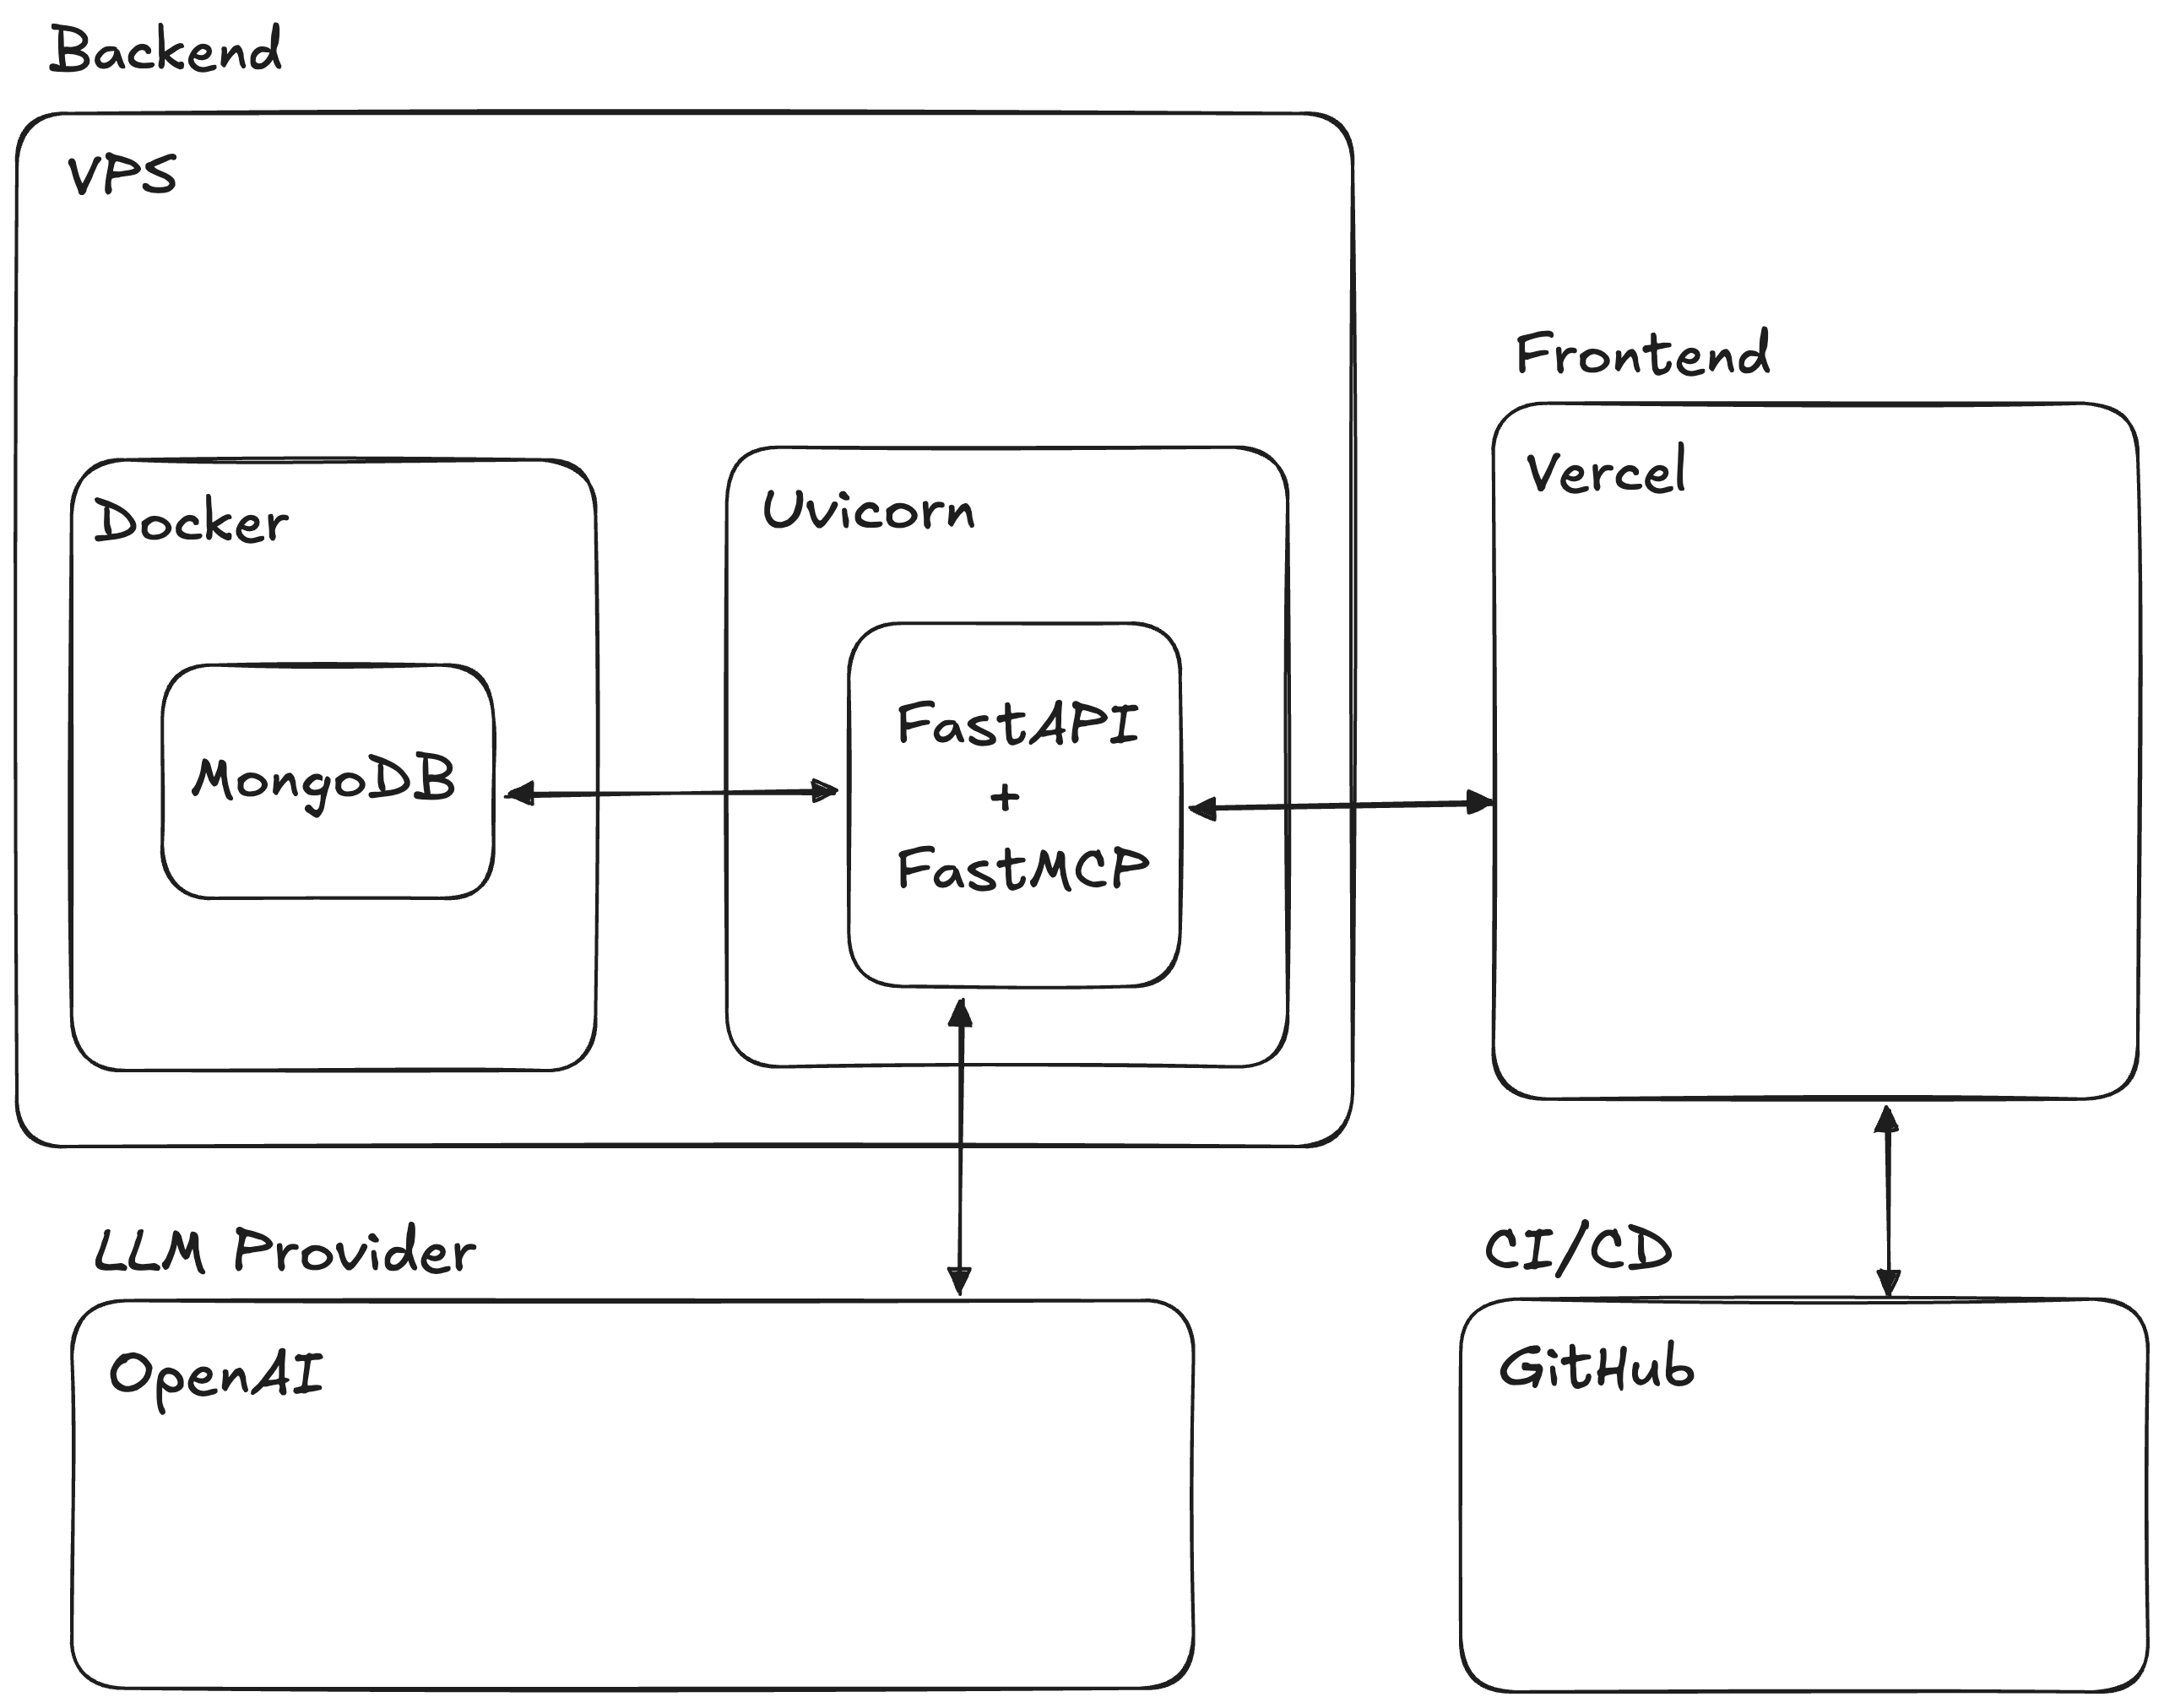
\includegraphics[width=0.9\textwidth]{imagenes/arch1.png}}
  %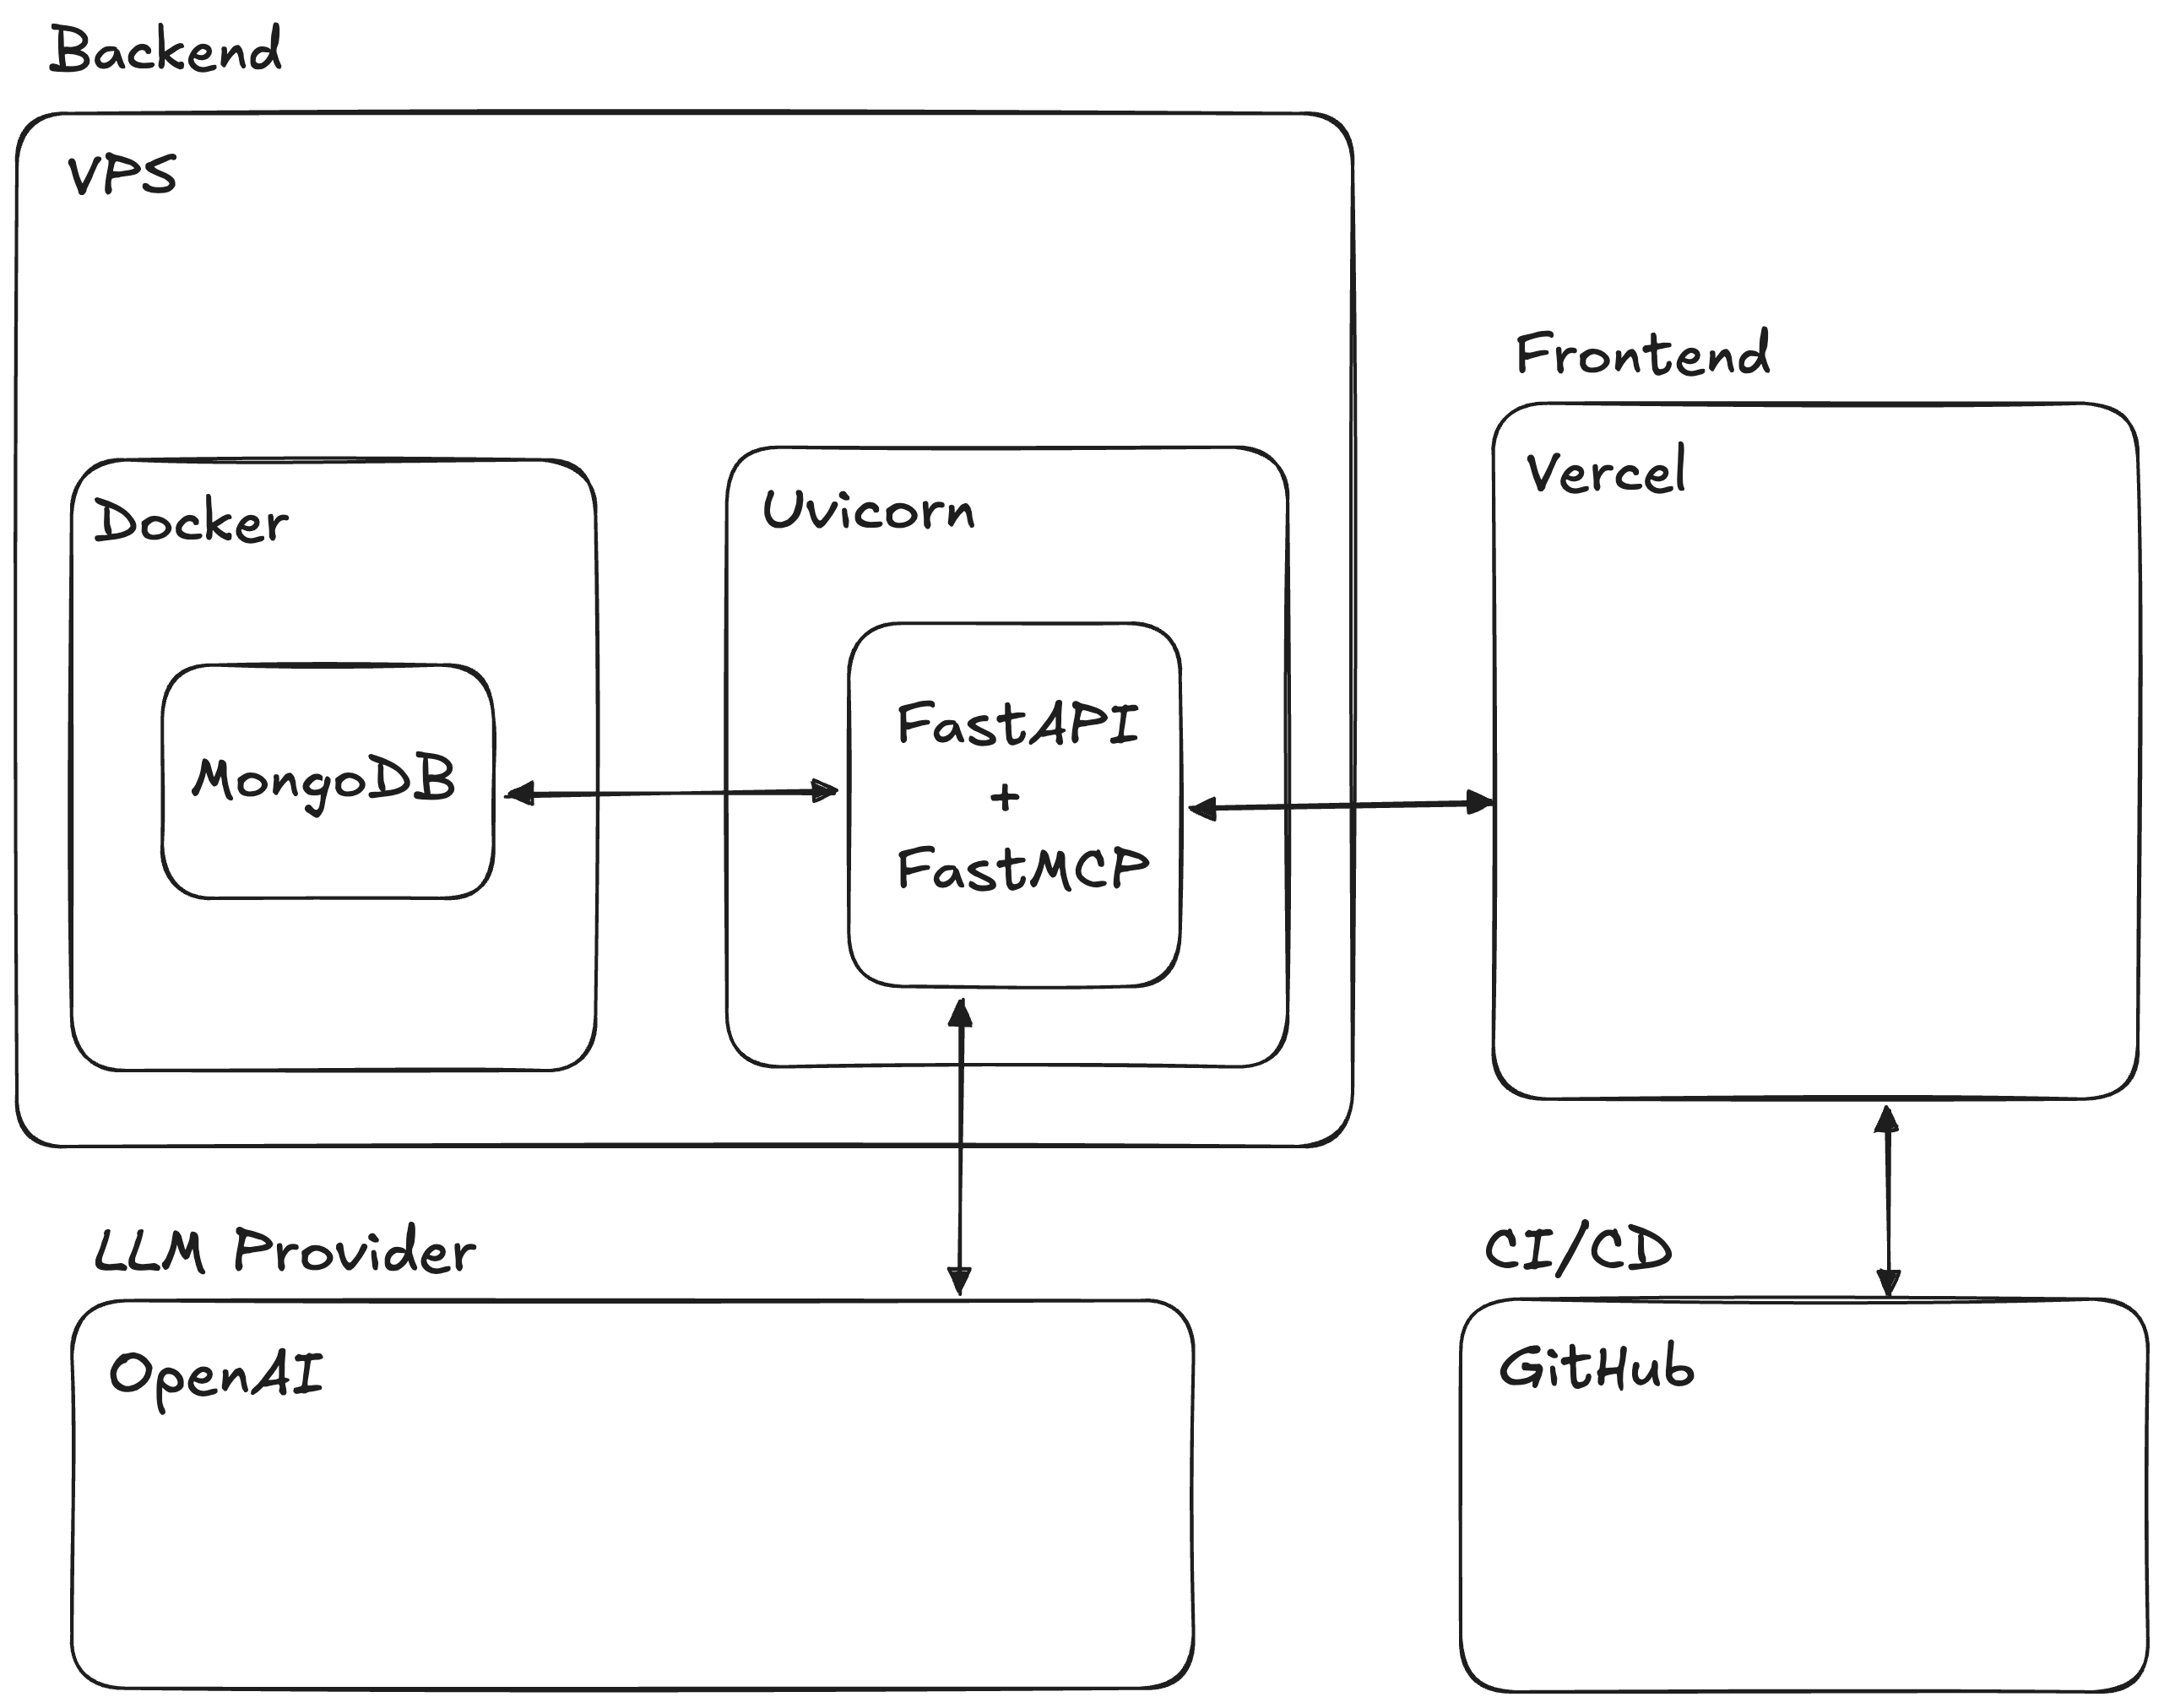
\includegraphics[width=0.9\textwidth]{imagenes/arch1.png}
  \caption{Arquitectura de la aplicación}
  \label{fig:arch1}
\end{figure}

\section{Backend}

El backend constituye el núcleo de la lógica de este trabajo. Se puede dividir en dos elementos: la base de datos MIMIC-IV almacenada en MongoDB con Docker, y la API RESTful con FastAPI que consulta datos, los procesa y los devuelve al cliente. También se encarga de llamar a los LLMs y a ejecutar el servidor MCP. Todo se aloja en un servidor personal y se accede por HTTPS gracias a Cloudflare Tunnels. A continuación profundizamos en esta parte del proyecto.

%\subsection{Almacenamiento de MIMIC-IV en MongoDB}
\subsection{MIMIC-IV en MongoDB}


Una de las tareas técnicas fundamentales del proyecto ha sido la migración del conjunto de datos, desde su formato original en archivos CSV comprimidos a una base de datos MongoDB. A continuación se explica todo el proceso.

\subsubsection{Entendiendo los datos}

MIMIC-IV recoge sus datos de distintas fuentes, y realiza todo un complejo proceso de conversión, transformación, anonimización, clasificación y corrección de los datos hasta obtener el resultado final \cite{MIMICIV_paper}.

\begin{figure}[H]
    \centering
    \fbox{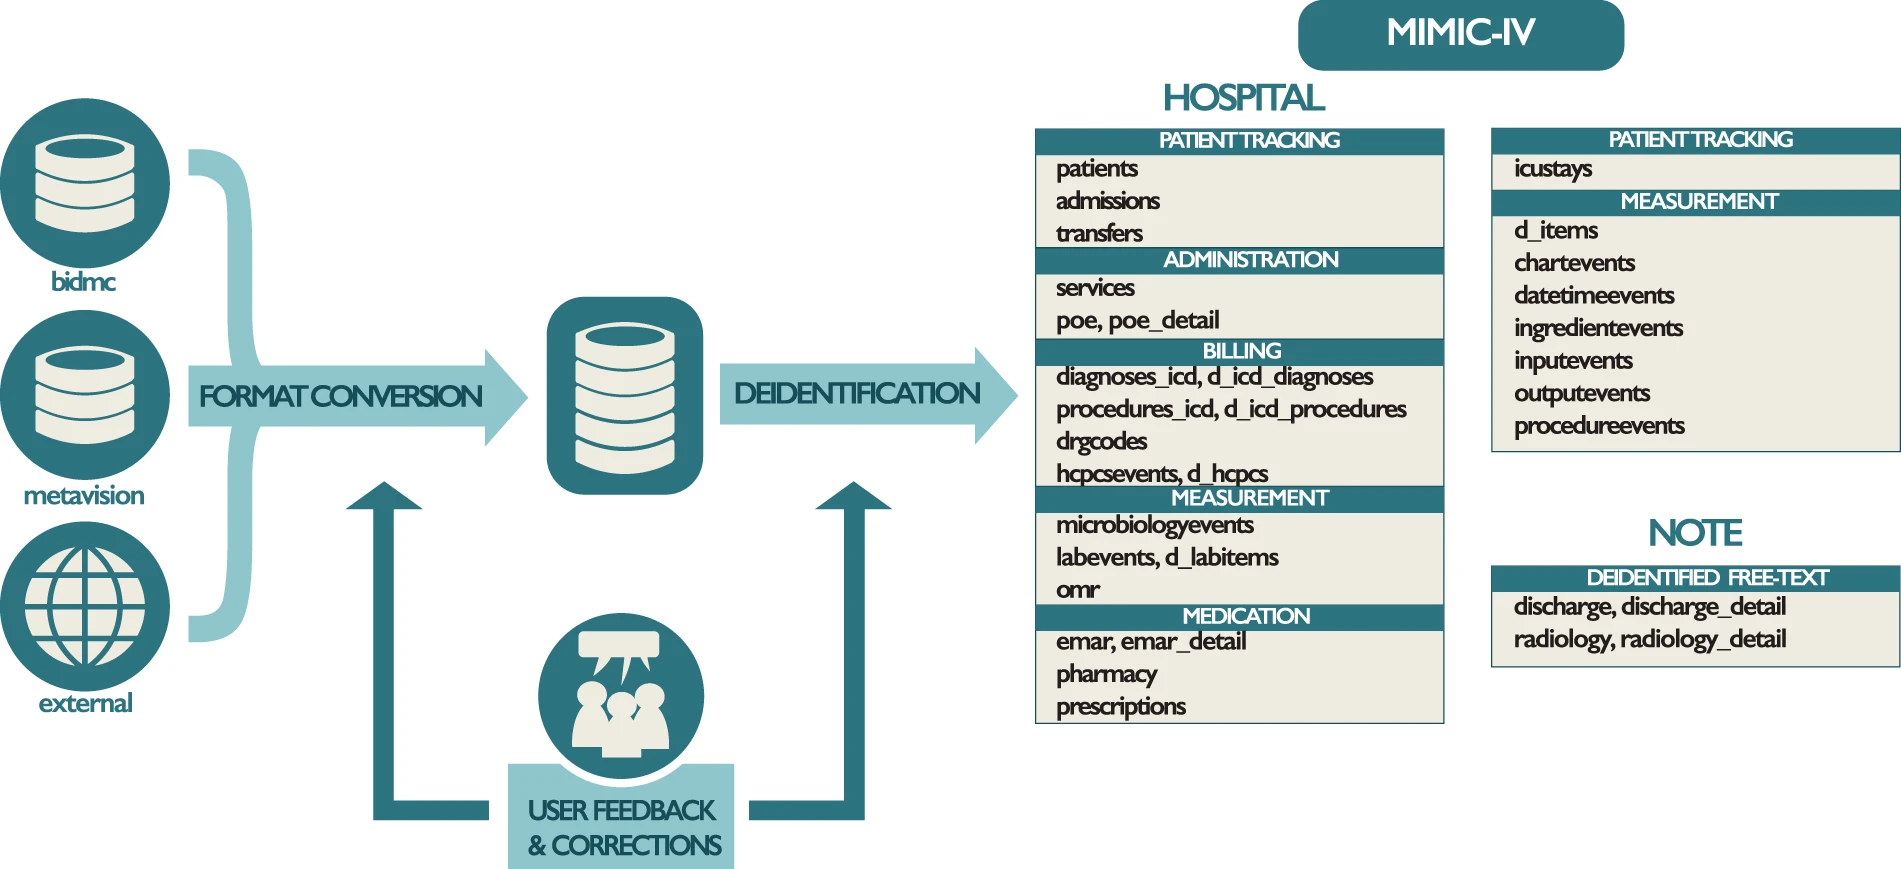
\includegraphics[width=0.95\textwidth]{imagenes/desarrolloMIMIC-IV.png}}
    %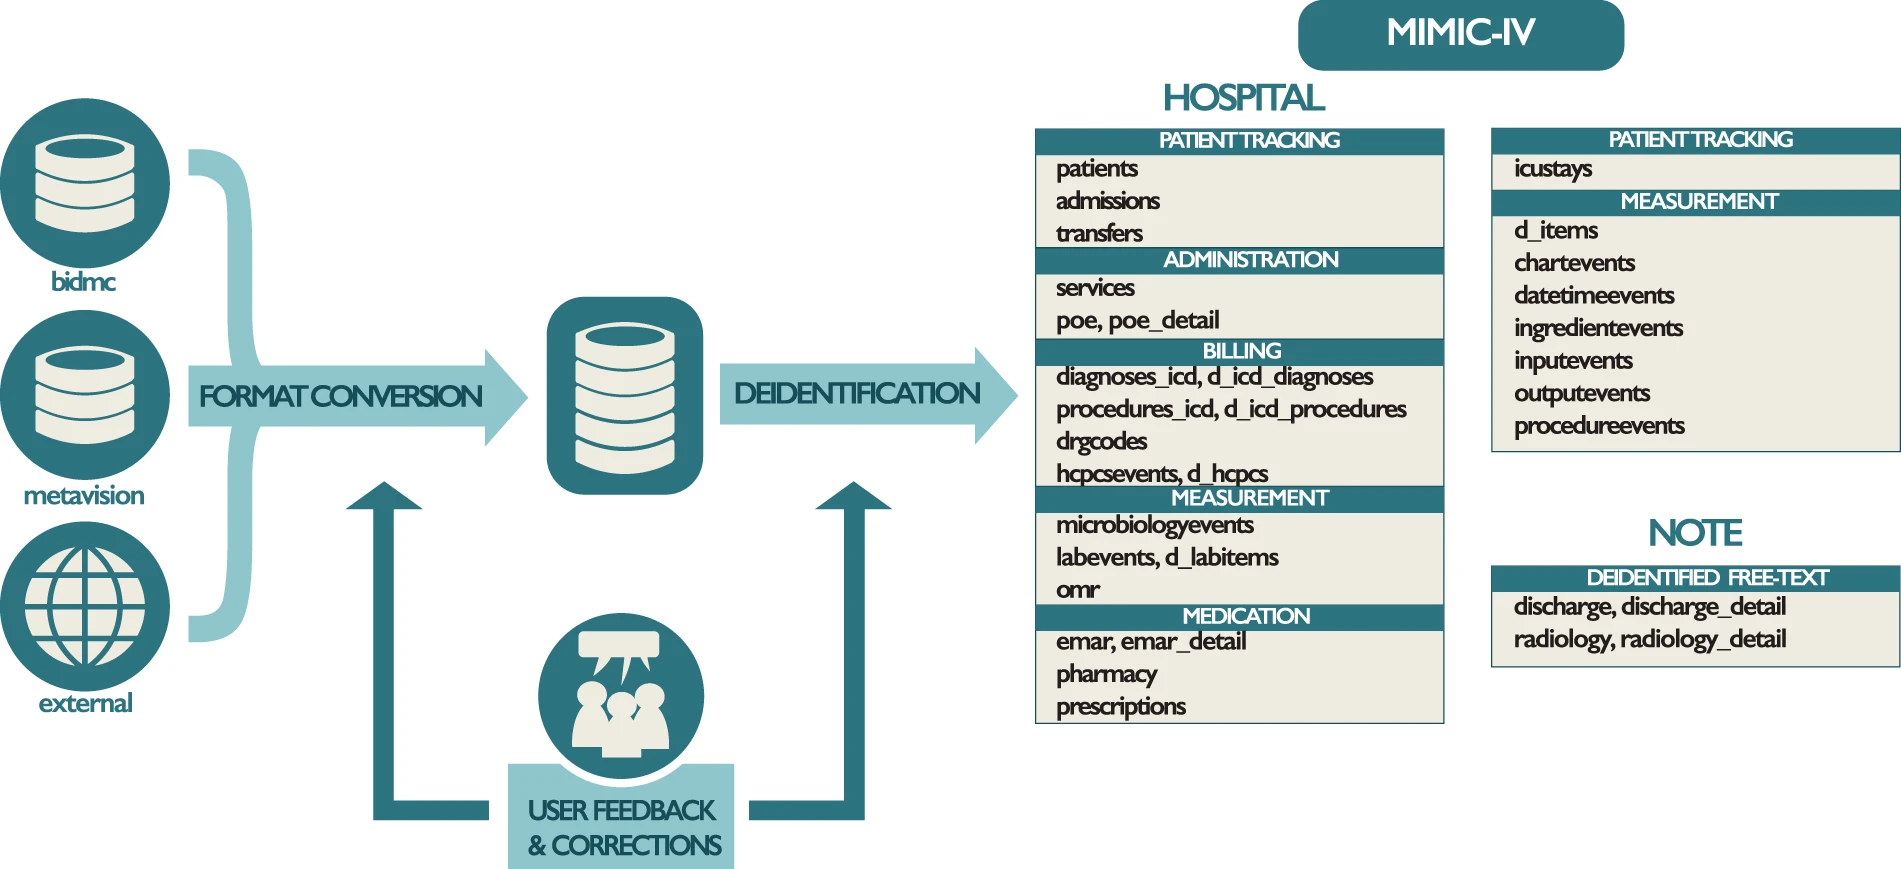
\includegraphics[width=0.95\textwidth]{imagenes/desarrolloMIMIC-IV.png}
    \caption{Resumen del proceso de desarrollo de MIMIC-IV.}
    \label{fig:desarrollo_mimiciv}
\end{figure}


Los datos, tal y como se han recibido, se estructuran módulos o ``carpetas", cada uno compuesto por diferentes tablas o ``archivos" que recogen distintos aspectos de la estancia hospitalaria del paciente. A continuación se resumen los dos módulos que se utilizan en el proyecto y sus tablas más relevantes:

\begin{itemize}
    \item \textbf{hosp}: Información hospitalaria general procedente del sistema de historia clínica electrónica. Incluye:
    \begin{itemize}
        \item \texttt{patients}: datos demográficos como sexo, edad y fecha de fallecimiento.
        \item \texttt{admissions}: detalles de los ingresos hospitalarios.
        \item \texttt{transfers}: movimientos de los pacientes entre distintas unidades.
        \item \texttt{labevents} y \texttt{d\_labitems}: resultados de laboratorio y su descripción.
        \item \texttt{microbiologyevents}: cultivos microbiológicos.
        \item \texttt{prescriptions}, \texttt{pharmacy}, \texttt{emar}, \texttt{emar\_detail}: información sobre prescripciones y administración de medicamentos.
        \item \texttt{diagnoses\_icd}, \texttt{d\_icd\_diagnoses}: diagnósticos realizados y codificados (ICD-9/10).
        \item \texttt{procedures\_icd}, \texttt{d\_icd\_procedures}: procedimientos realizados y codificados (ICD-9/10).
        \item \texttt{hcpcsevents}, \texttt{d\_hcpcs}, \texttt{drgcodes}: información de facturación y codificación hospitalaria.
        \item \texttt{services}: servicios hospitalarios responsables del paciente.
        \item \texttt{poe}, \texttt{poe\_detail}: órdenes médicas realizadas por los profesionales.
        \item \texttt{provider}, \texttt{omr}: información sobre proveedores y registros médicos online.
    \end{itemize}
    \item \textbf{icu}: Datos recogidos específicamente durante la estancia en la UCI, provenientes del sistema clínico MetaVision. Incluye:
    \begin{itemize}
        \item \texttt{icustays}: información sobre las estancias en UCI.
        \item \texttt{chartevents}: registros detallados de constantes, procedimientos, observaciones y eventos clínicos.
        \item \texttt{inputevents}, \texttt{ingredientevents}: administración de fluidos, nutrición y medicamentos intravenosos.
        \item \texttt{outputevents}: registros de salidas del paciente (orina, drenajes, etc.).
        \item \texttt{procedureevents}: procedimientos realizados en UCI.
        \item \texttt{datetimeevents}: eventos documentados con fecha y hora.
        \item \texttt{d\_items}: diccionario de variables y conceptos registrados en los eventos.
        \item \texttt{caregiver}: identificadores de los profesionales sanitarios en UCI.
    \end{itemize}
\end{itemize}



En nuestro caso, utilizamos estos dos módulos pero hay más, como \textbf{ed} (emergency department), \textbf{cxr} (radiografías de tórax) y \textbf{note} (notas clínicas desidentificadas), que amplían la información disponible para cada paciente.

Un aspecto fundamental para trabajar con MIMIC-IV es la correcta utilización de los campos identificadores que permiten relacionar la información entre tablas y reconstruir la trayectoria clínica de cada paciente:

\begin{itemize}
    \item \texttt{subject\_id}: identificador único de paciente, presente en prácticamente todas las tablas. Permite agrupar toda la información relativa a una misma persona a lo largo de distintas estancias y episodios.
    \item \texttt{hadm\_id}: identificador único de cada ingreso hospitalario. Cada hospitalización de un paciente tiene uno distinto, lo que permite diferenciar varios ingresos de la misma persona y asociar eventos, pruebas y tratamientos concretos a cada episodio.
    \item \texttt{stay\_id} (en ICU): identifica de forma única cada estancia en la UCI, permitiendo enlazar los eventos críticos de cuidados intensivos.
    \item Otros identificadores secundarios: \texttt{specimen\_id} (muestras de laboratorio), \texttt{pharmacy\_id}, \texttt{order\_provider\_id} (profesional que ordena una prueba o medicación), \texttt{itemid} (tipo de medición o concepto registrado), entre otros.
\end{itemize}

Además de todos estos datos, los tutores del trabajo proporcionaron otro archivo \texttt{icd\_equivalencias}, el cual contiene las equivalencias entre códigos ICD-9 e ICD-10. Los códigos ICD (International Classification of Diseases) son el estándar internacional para clasificar enfermedades, diagnósticos y procedimientos médicos. Esta tabla permite unificar datos codificados en ambas versiones y aporta una clasificación jerárquica organizada en capítulos (chapters), supersecciones (super sections) y secciones (sections). Por ejemplo, el código ICD-9 ``0090'' (Infectious colitis, enteritis, and gastroenteritis) se mapea al ICD-10 ``A09'' y se clasifica dentro del capítulo ``A'' (Certain infectious and parasitic diseases), supersección ``A00-A09'' (Intestinal infectious diseases) y sección ``A09'' (Infectious gastroenteritis and colitis, unspecified). Esta estructura facilita el análisis y visualización de diagnósticos por categorías médicas.

En conclusión, toda esta estructura modular nos permite, a nivel de paciente, reconstruir de forma detallada la trayectoria clínica, desde su ingreso hasta el alta, pasando por episodios críticos, pruebas, tratamientos y evolución. A nivel global, las posibilidades son enormes, para calcular estadísticas, visualizaciones, y todo tipo de agregaciones de las que se pueda extraer conocimiento. Para más detalles sobre los datos, puede consultarse la documentación oficial de MIMIC-IV \cite{MIMICIV_docs}.

\subsubsection{Desplegando MongoDB}

Para el despliegue de MongoDB se utilizan dos contenedores Docker, en distintos puertos, uno para la versión completa del conjunto de datos, y otro para la versión demo, facilitando así la realización de pruebas sin tener que lidiar con los cientos de millones de datos de la versión completa. Como apoyo al desarrollo, y también en forma de contenedores, se despliegan las herramientas de interfaz gráfica: Portainer para Docker \cite{portainer_ce} y Mongo Express para las bases de datos \cite{mongo_express}. 


\begin{figure}[H]
  \centering
  \fbox{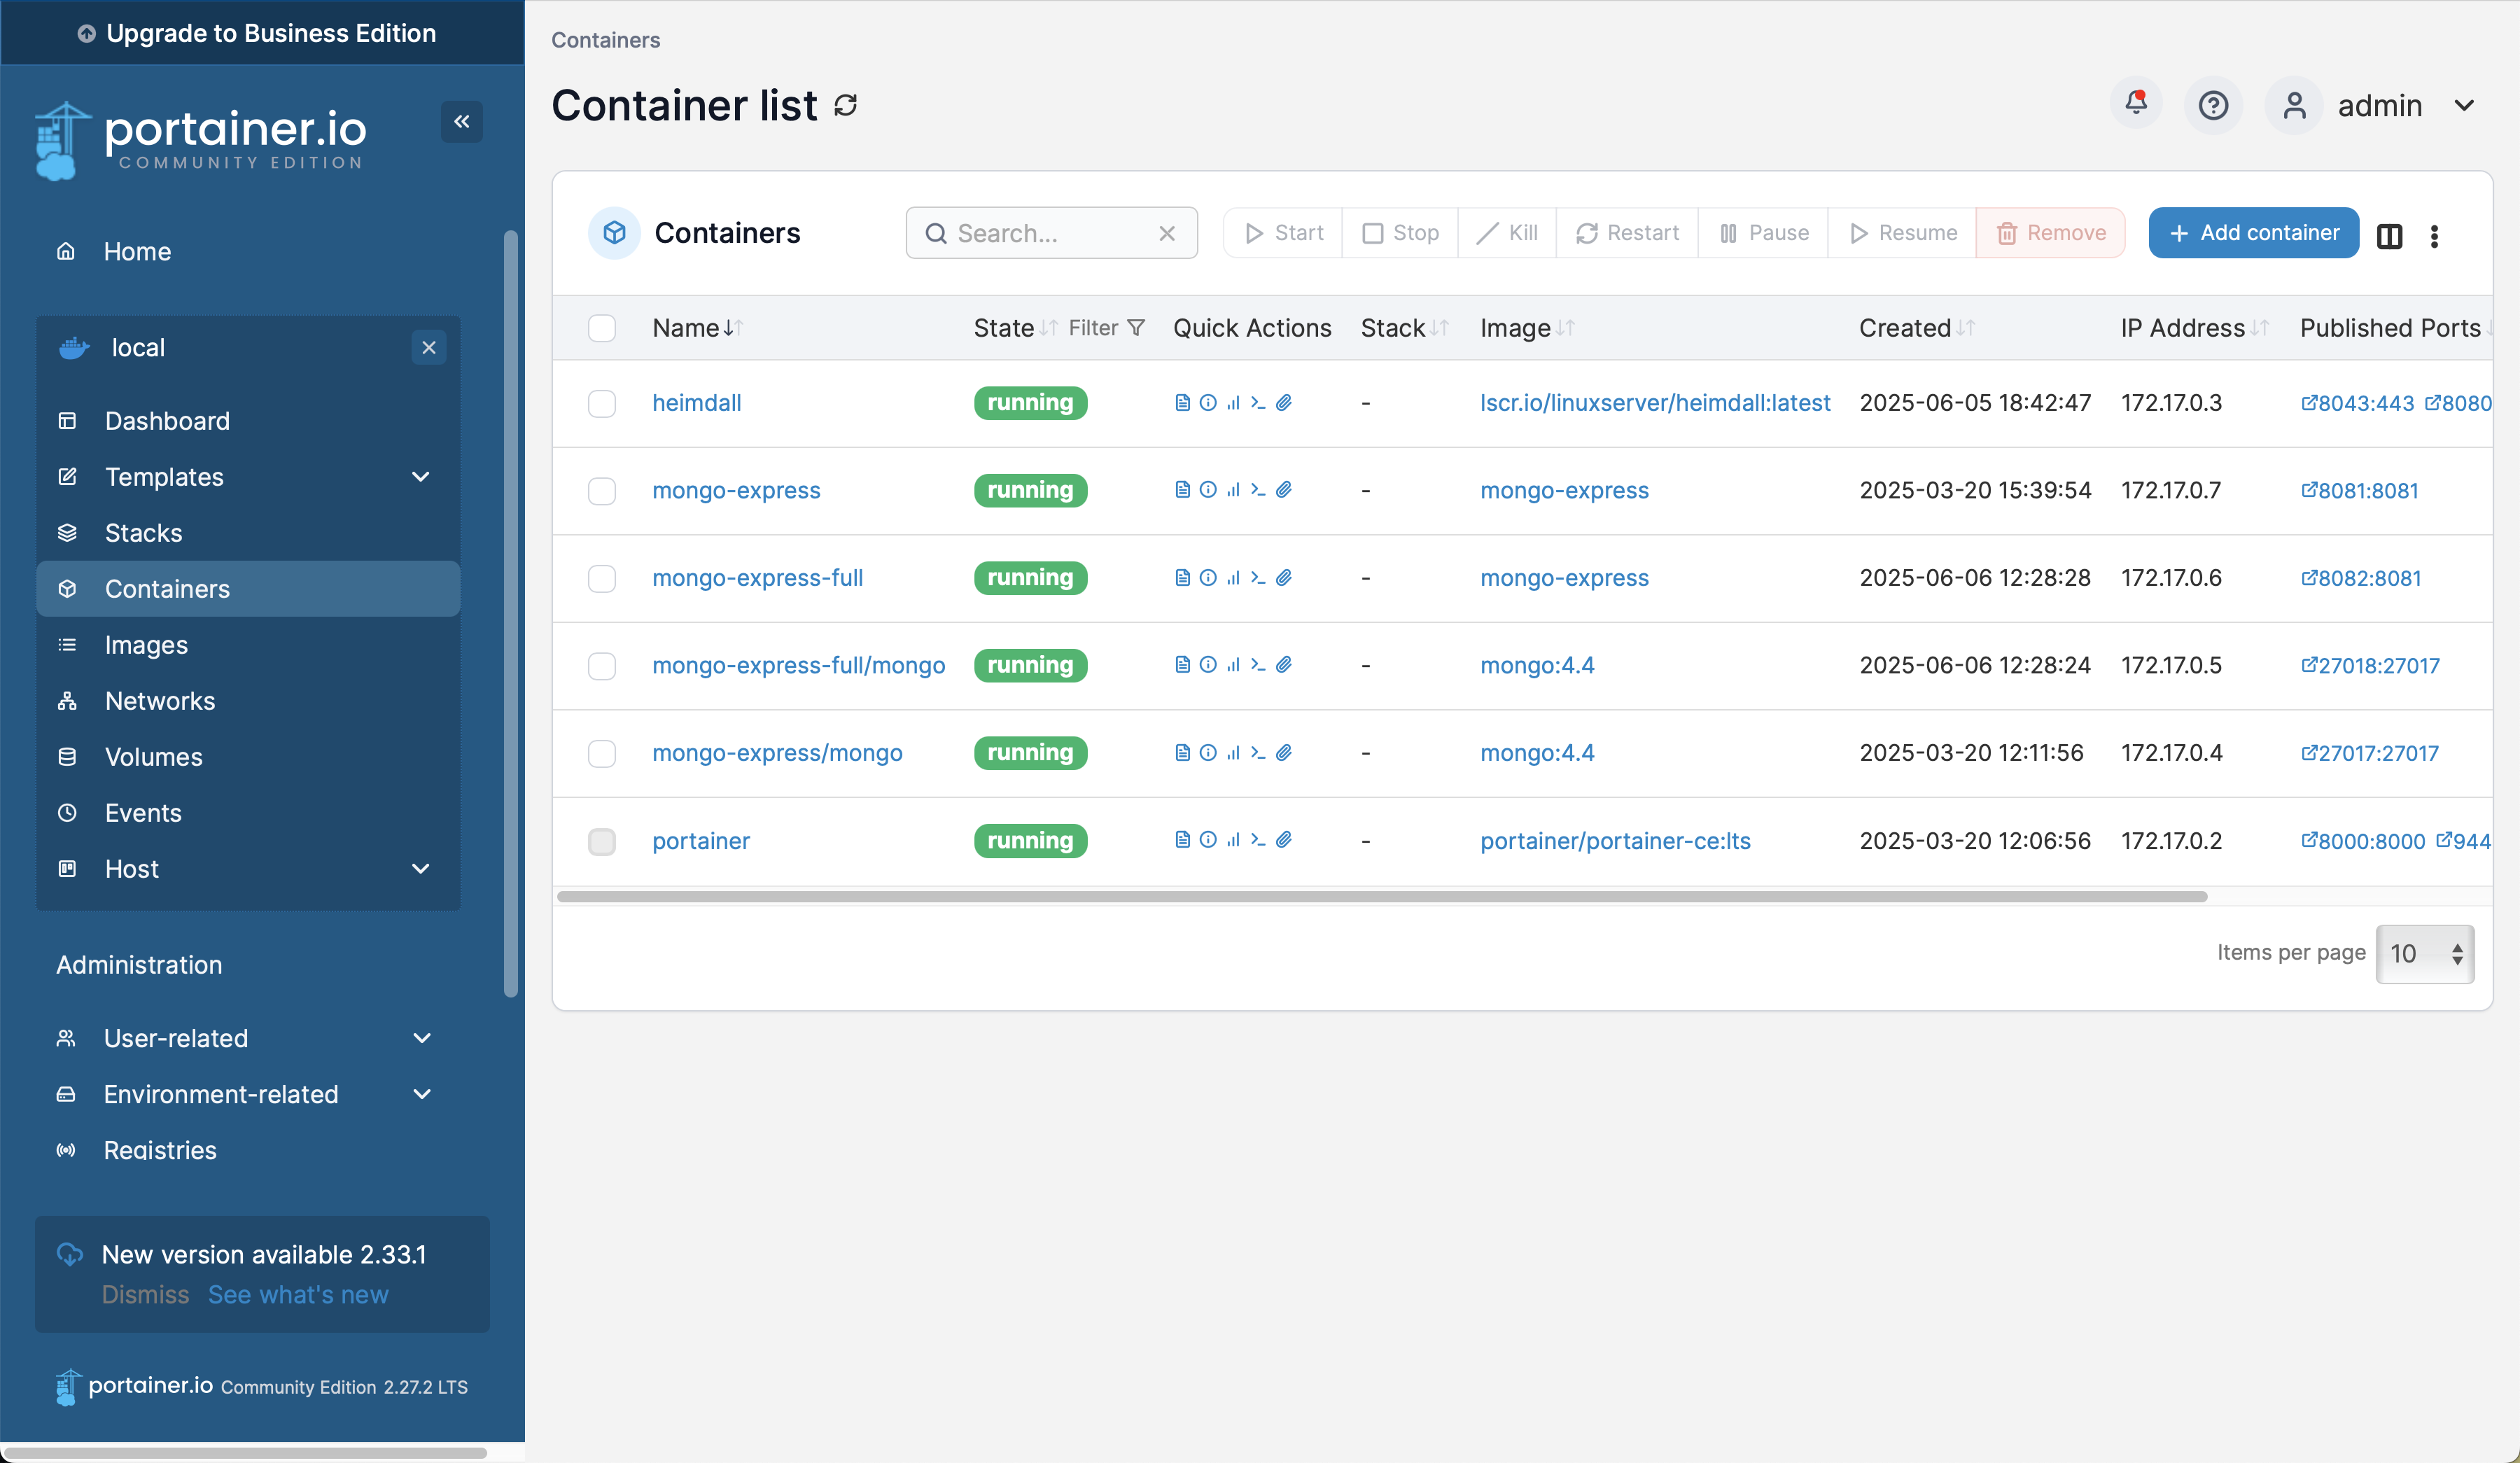
\includegraphics[width=1\textwidth]{imagenes/screenshot3.png}}
  %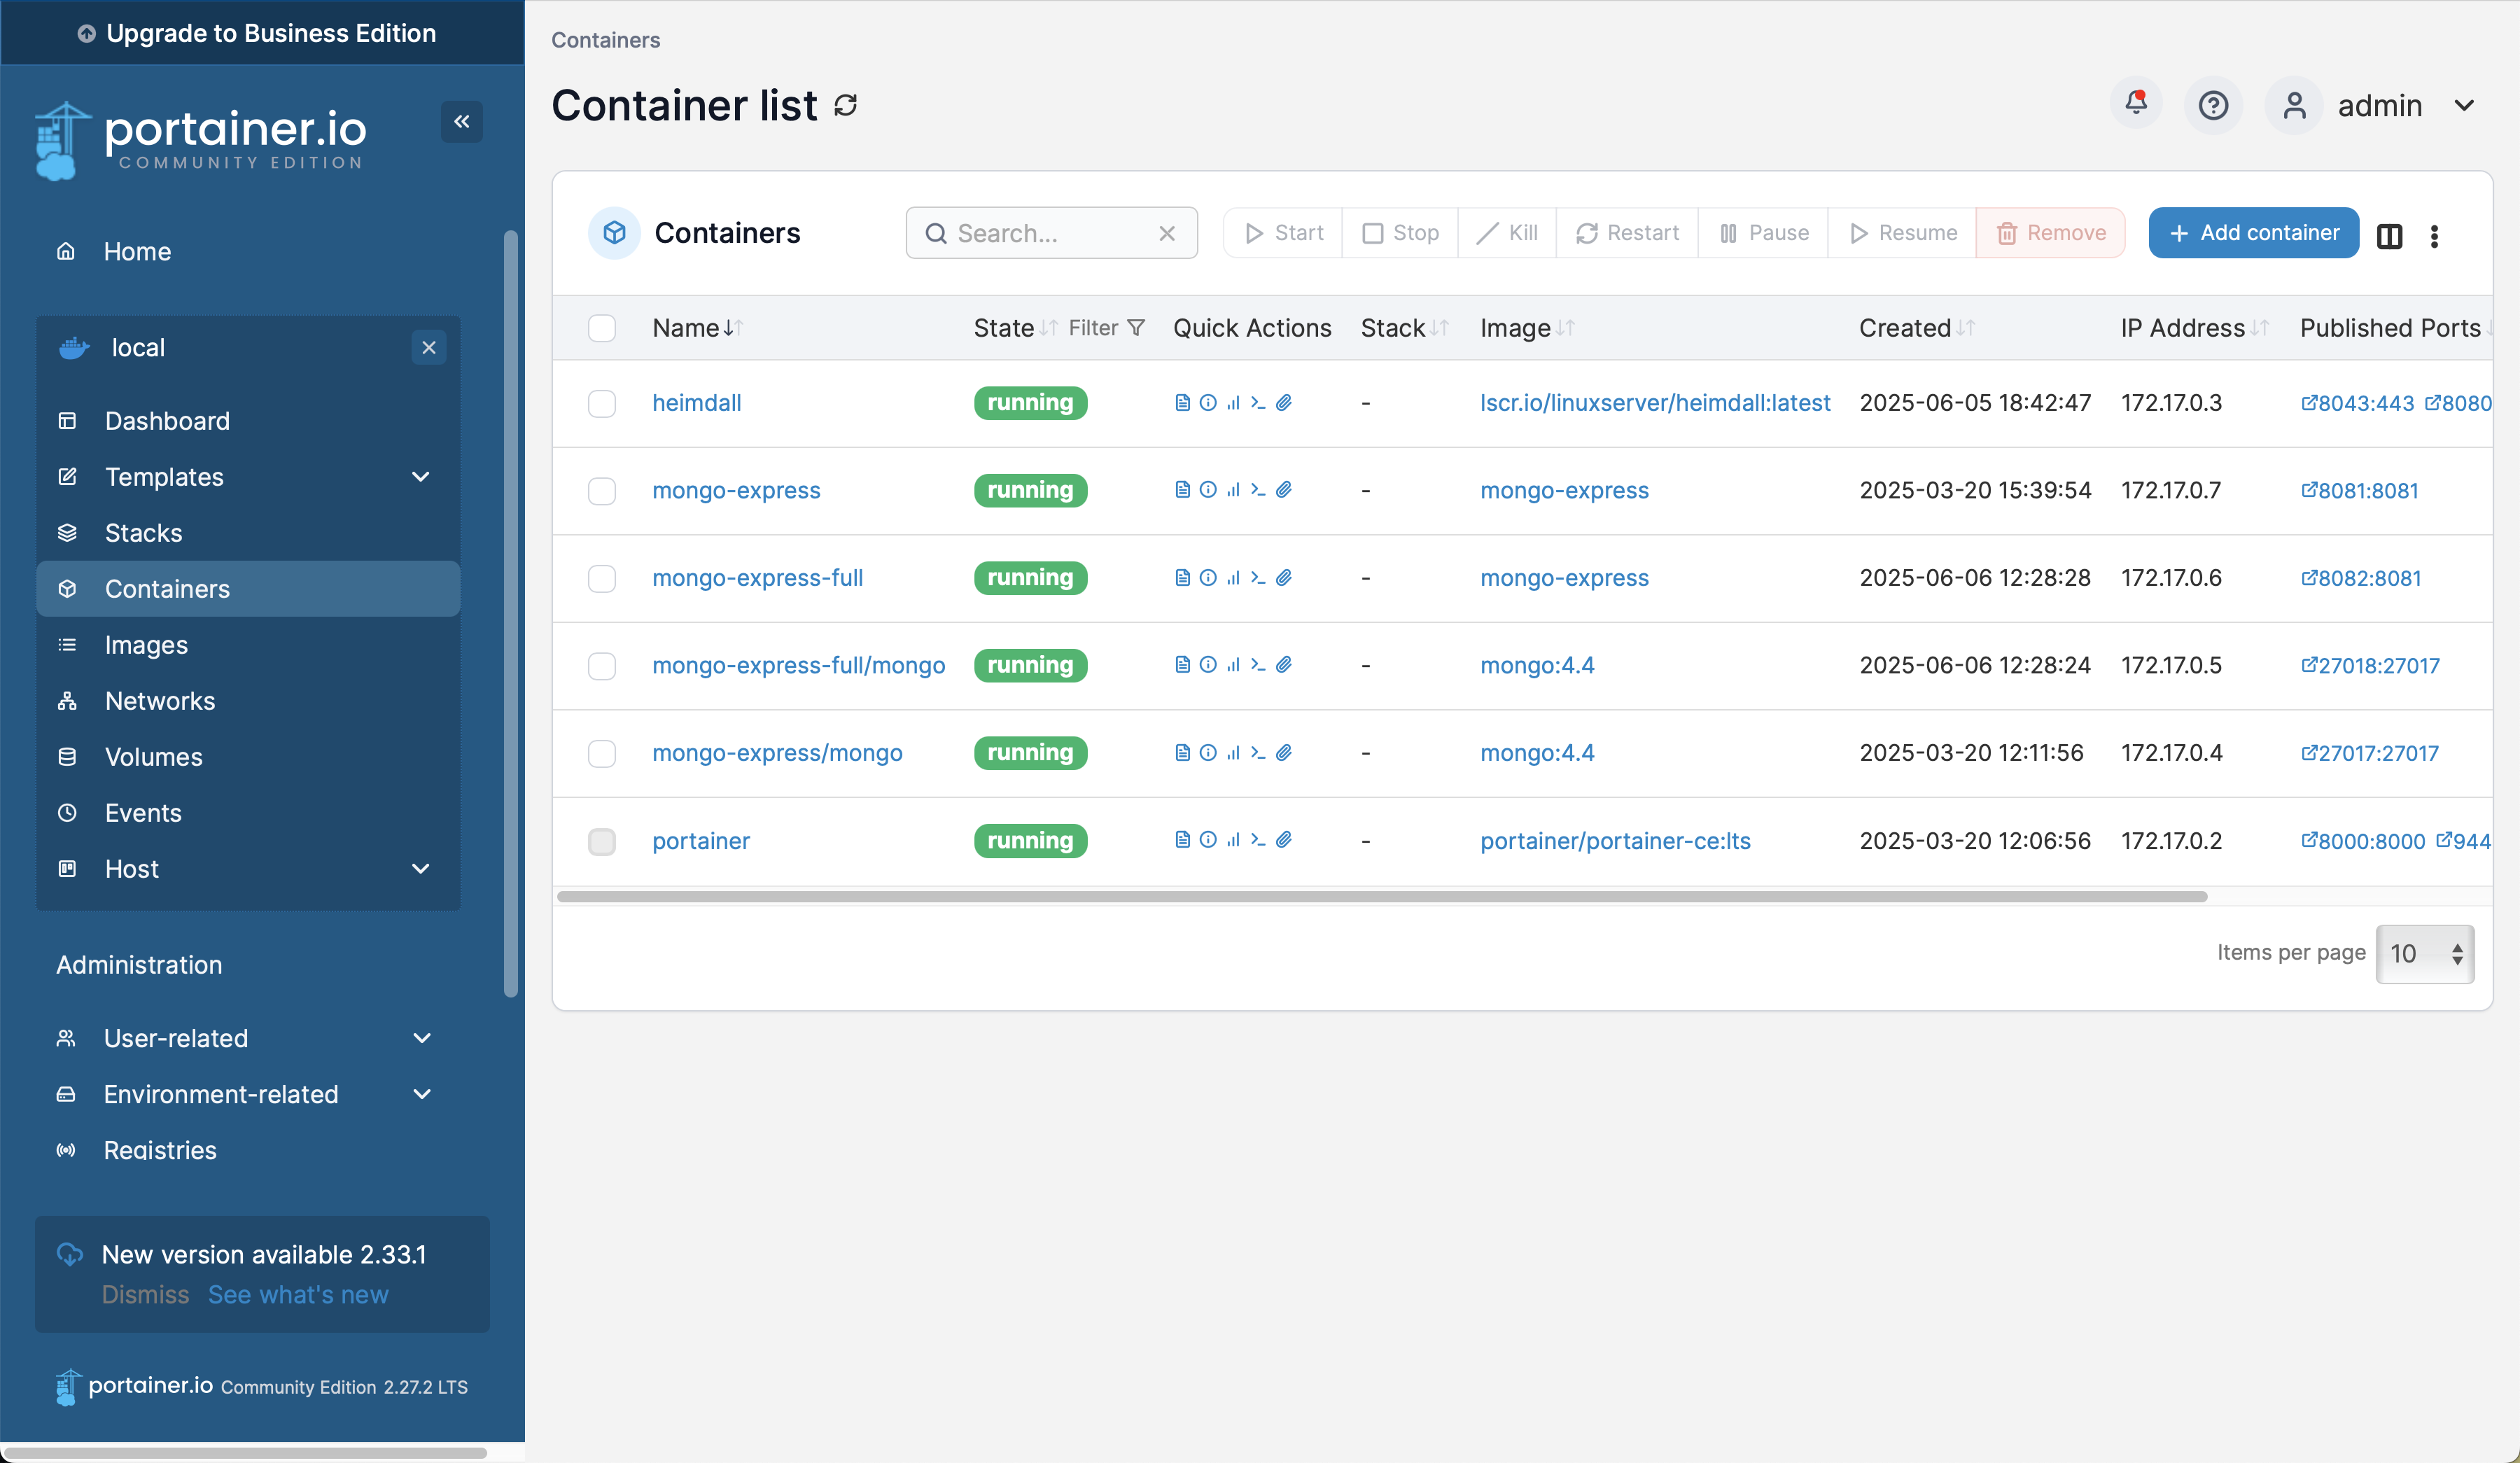
\includegraphics[width=1\textwidth]{imagenes/screenshot3.png}
  \caption{Captura de pantalla de Portainer}
  \label{fig:screenshot3}
\end{figure}


% --------------------
\subsubsection{El proceso de migración}

Se realizó mediante scripts de Python utilizando la librería \texttt{pandas} para la lectura de archivos CSV y \texttt{pymongo} para la inserción en MongoDB. Cada fila del CSV se convierte en un archivo JSON/BSON \cite{mongojsonbson} en MongoDB, donde cada columna es un campo del documento, y cada archivo CSV completo acaba siendo una colección de documentos. Podemos entenderlo mejor, pensando que cada archivo CSV es equivalente a una tabla de una base de datos relacional, y observando la siguiente figura \ref{fig:equivalenciasql}.

\begin{figure}[H]
  \centering
  \fbox{\includegraphics[width=0.8\textwidth]{imagenes/mongodb-vs-sql-1.png}}
  %\includegraphics[width=0.8\textwidth]{imagenes/mongodb-vs-sql-1.png}
  \caption{Equivalencia entre conceptos SQL y NoSQL \cite{equisqlfoto}}
  \label{fig:equivalenciasql}
\end{figure}

Los nombres de las colecciones recibieron el formato \texttt{\textless módulo\textgreater\_\textless tabla\textgreater}. Por ejemplo: \texttt{hosp\_patients}, \texttt{icu\_procedureevents}, etc.

\begin{figure}[H]
  \centering
  \fbox{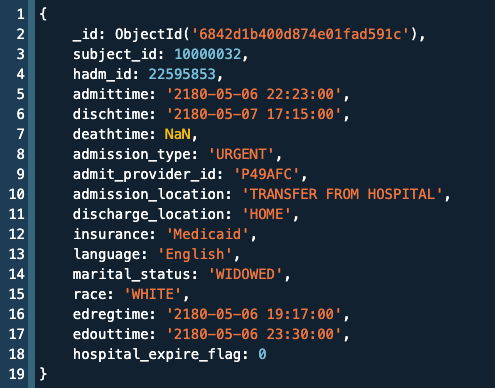
\includegraphics[width=0.6\textwidth]{imagenes/ej_admission.png}}
  %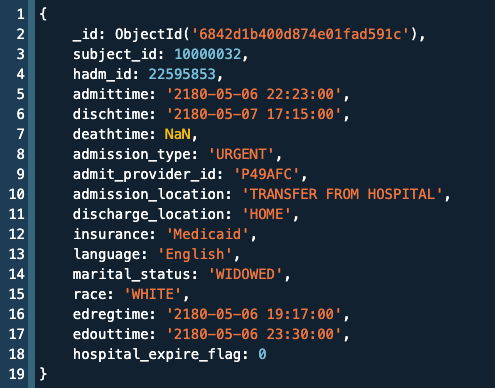
\includegraphics[width=0.6\textwidth]{imagenes/ej_admission.png}
  \caption{Ejemplo de un documento de \texttt{hosp\_admissions}}
  \label{fig:screenshot3}
\end{figure}

Una vez entendida la estructura de los datos de MIMIC-IV, la equivalencia de los archivos CSV a documentos y colecciones de MongoDB, la base de datos ejecutandose con Docker y los scripts preparados, era momento de realizar la migración. 

Todo este proceso se realizó dos veces, para dos versiones distintas de MIMIC-IV: la versión completa, cuyo acceso está restringido y contiene múltiples GBs de información, y la versión demo, que es un subset de 100 pacientes y es de acceso libre \cite{MIMICIV_Demo}. Para la versión completa, el procesamiento se tuvo que realizar por chuncks para evitar el desbordamiento de memoria, que fue un problema recurrente debido a la cantidad masiva de datos.

\begin{figure}[H]
    \centering
    \fbox{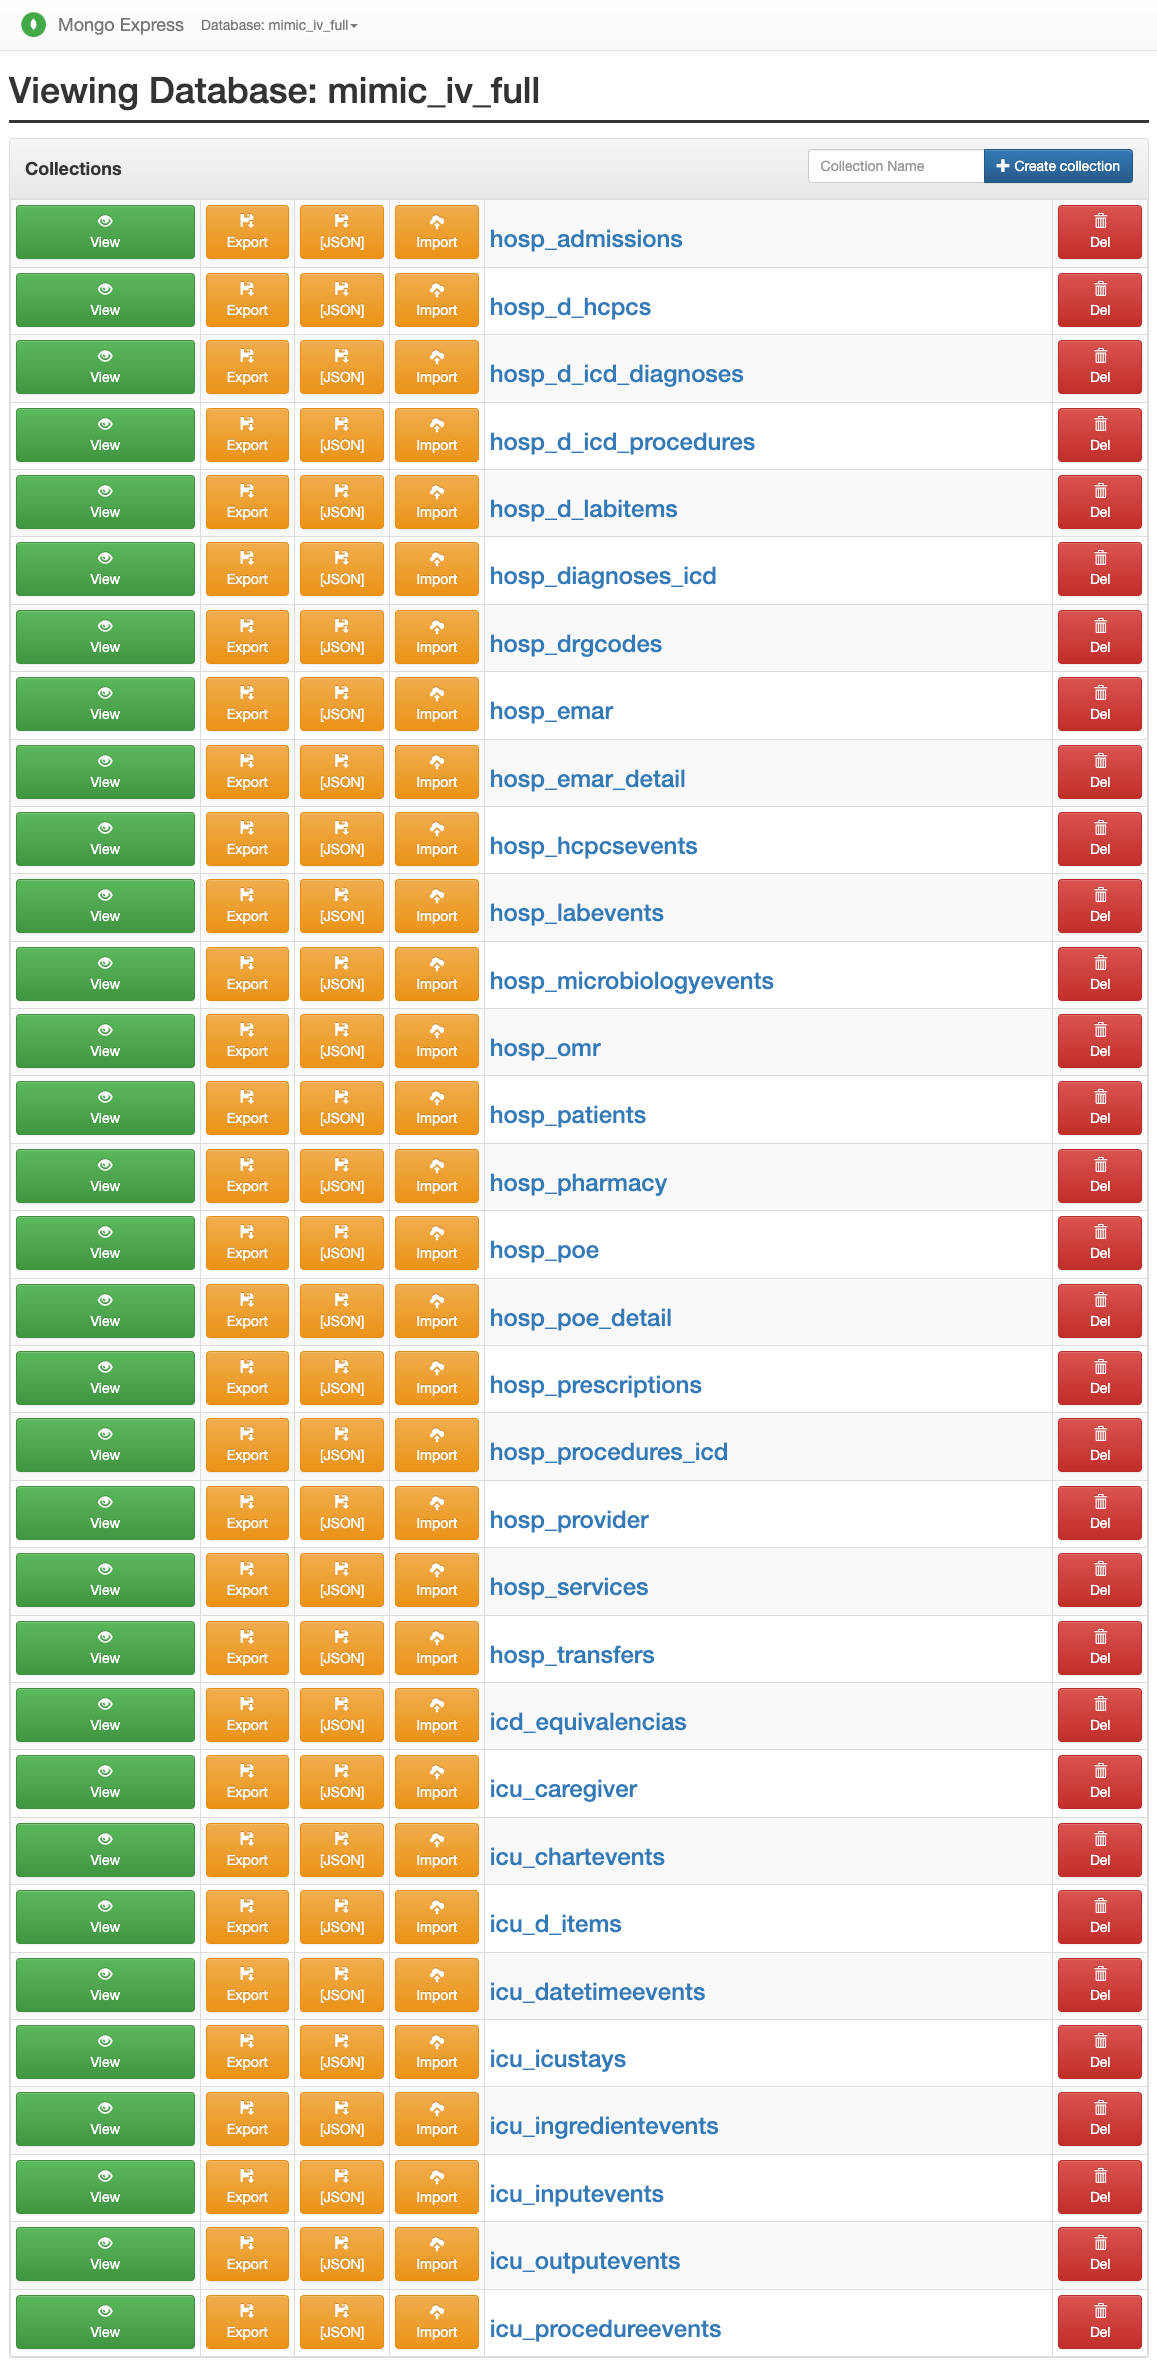
\includegraphics[width=0.8\textwidth]{imagenes/db_full_list.png}}
    %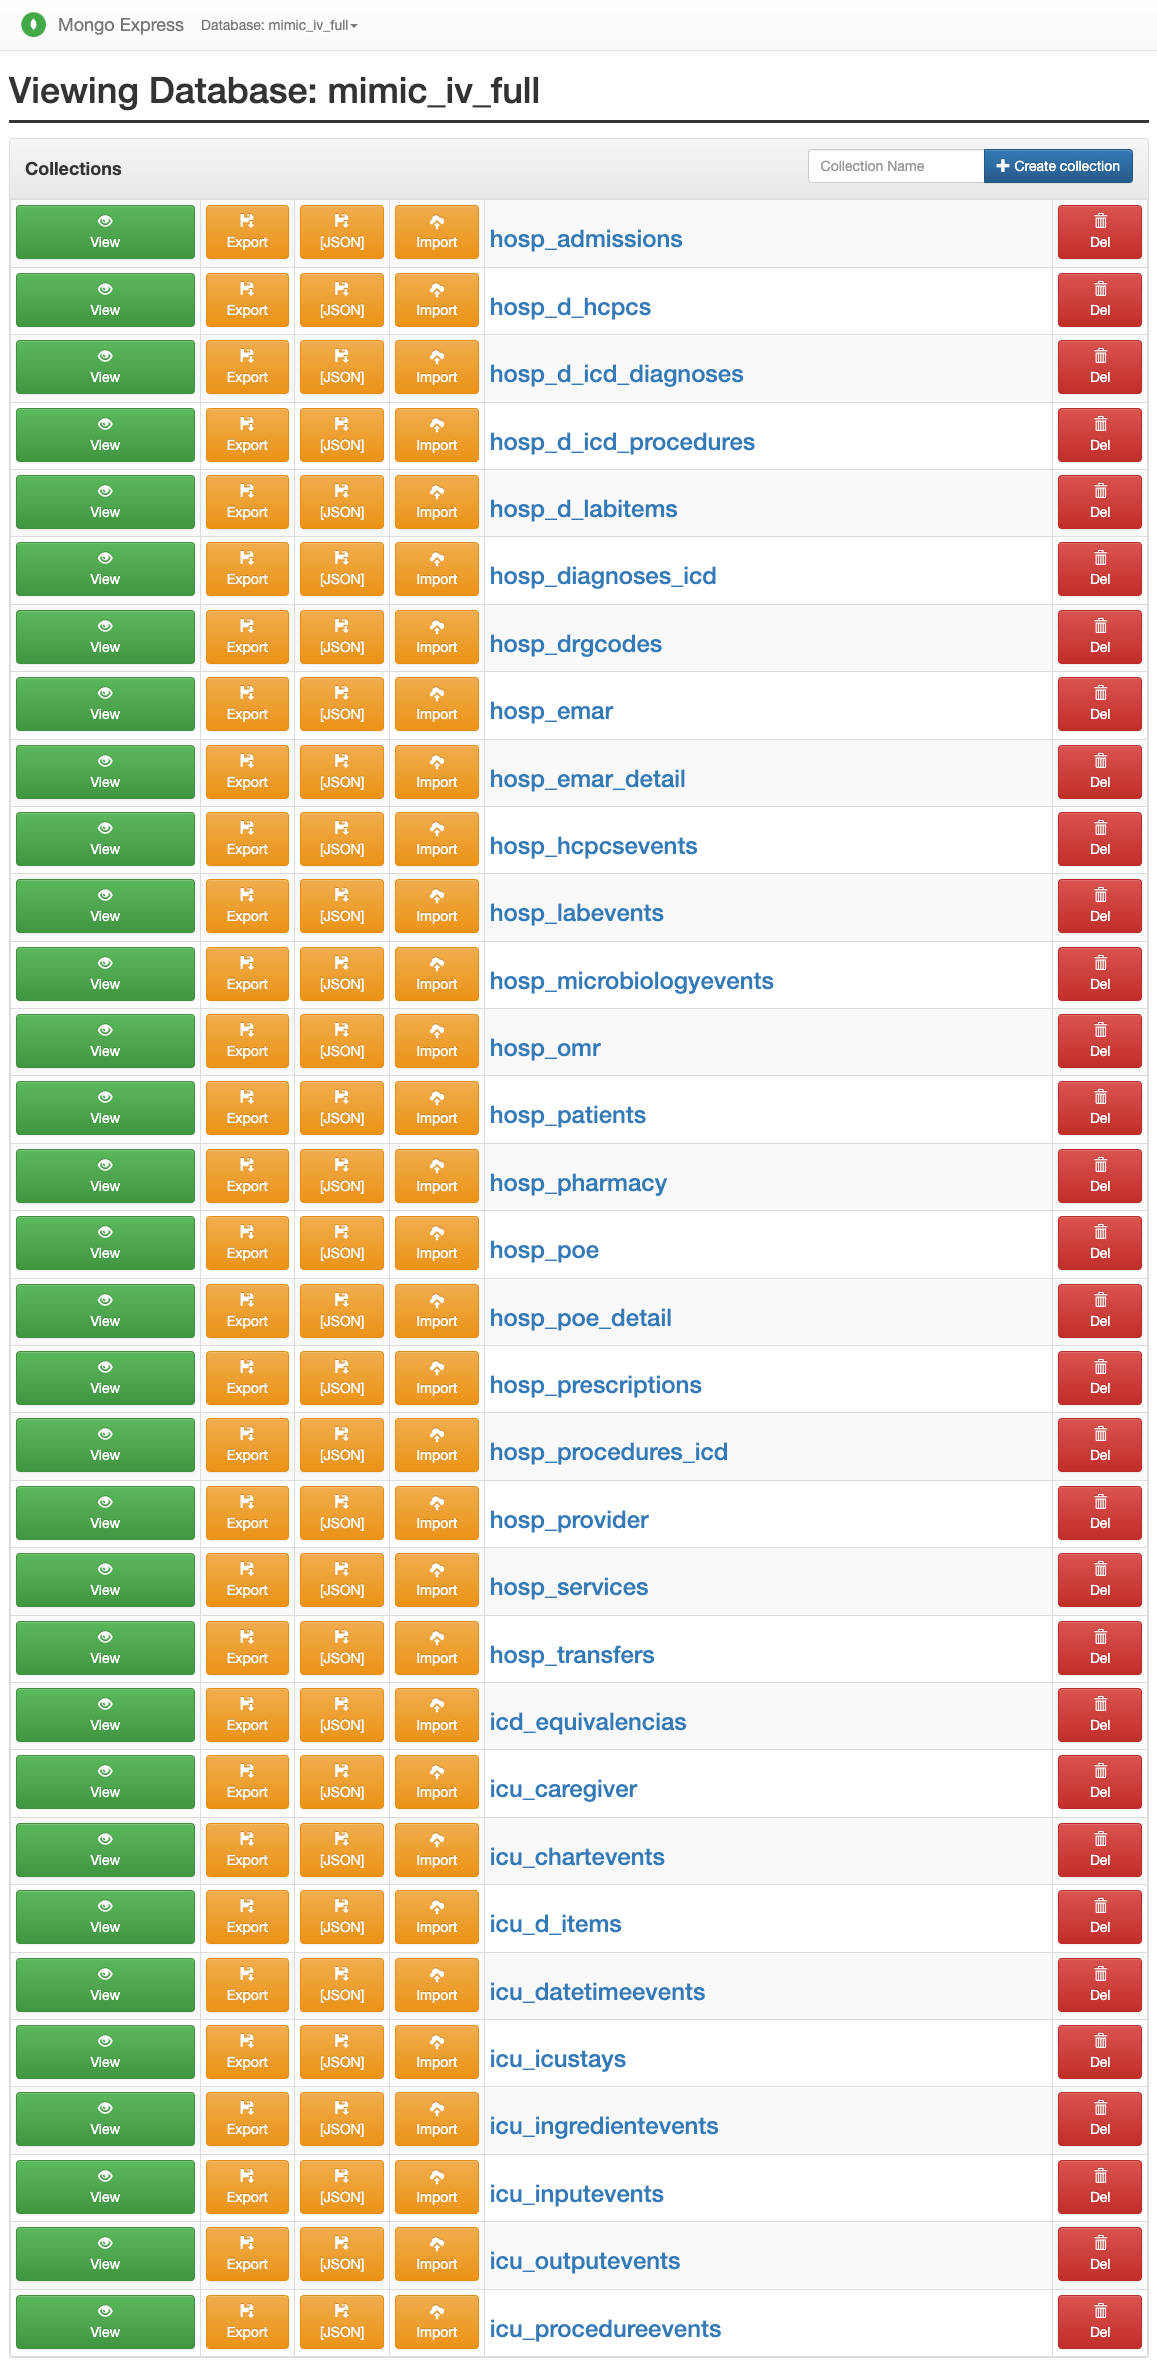
\includegraphics[width=0.8\textwidth]{imagenes/db_full_list.png}
    \caption{Colecciones resultantes tras la importacion. Captura de pantalla de la interfaz de Mongo Express.}
    \label{fig:db_full_list}
\end{figure}

\begin{figure}[H]
    \centering
    \fbox{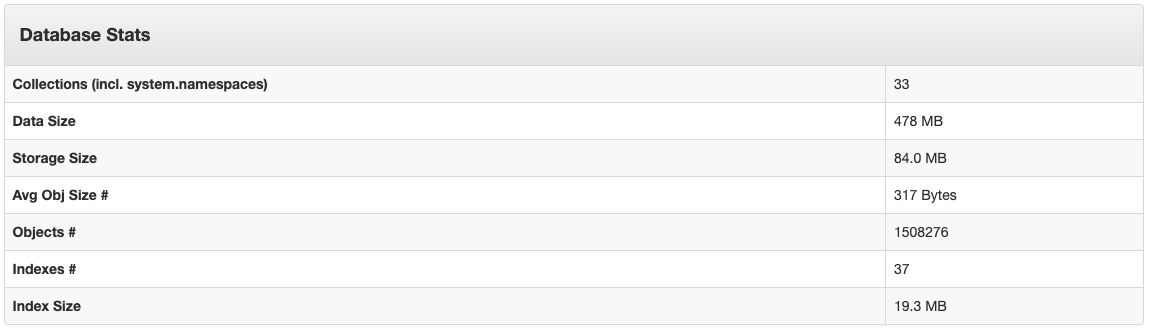
\includegraphics[width=1\textwidth]{imagenes/stats_demo.png}}
    %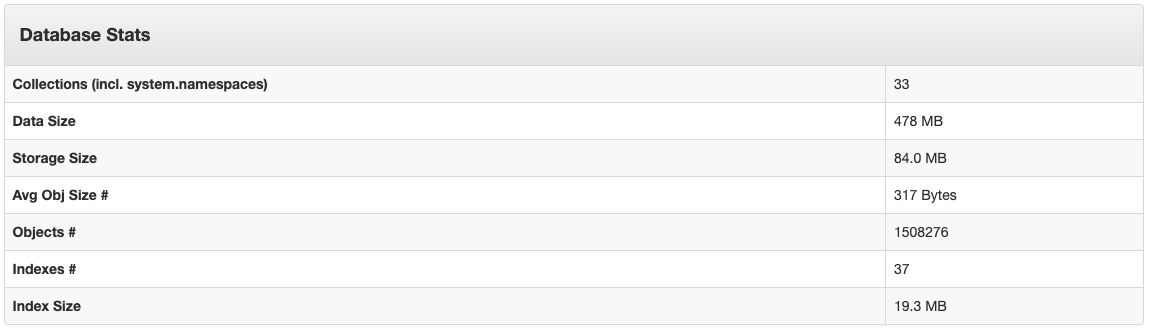
\includegraphics[width=1\textwidth]{imagenes/stats_demo.png}
    \caption{Estadísticas de la versión demo de la base de datos.}
    \label{fig:stats_demo}
\end{figure}

\begin{figure}[H]
    \centering
    \fbox{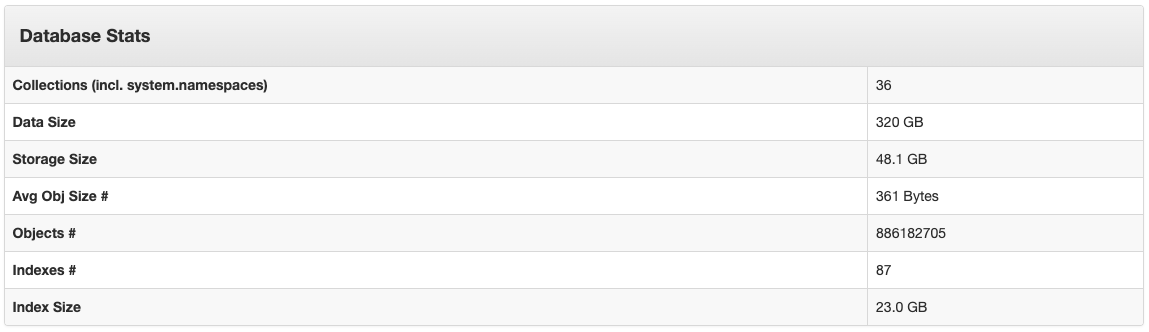
\includegraphics[width=1\textwidth]{imagenes/stats_full.png}}
    %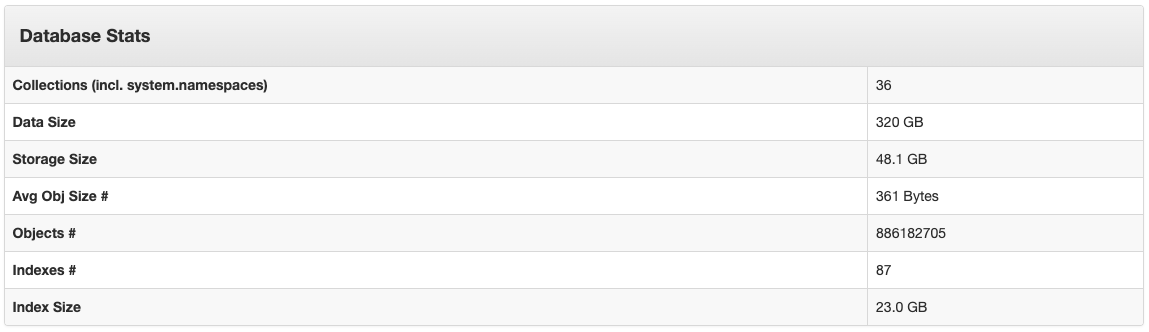
\includegraphics[width=1\textwidth]{imagenes/stats_full.png}
    \caption{Estadísticas de la versión completa de la base de datos.}
    \label{fig:stats_full}
\end{figure}


Además de las colecciones base que obtenemos de MIMIC-IV, a lo largo del proyecto se agregaron manualmente algunas más, necesarias tanto para pruebas como para algunas visualizaciones, de las que se hablará más tarde. Por eso, las estadísticas mostradas en las dos figuras anteriores, no coinciden exactamente con las del estado inicial del proyecto. 

También se crearon manualmente múltiples índices para optimizar el rendimiento de las consultas. Los índices en MongoDB funcionan de manera similar a los índices de un libro: crean estructuras de datos ordenadas que permiten localizar documentos específicos sin tener que examinar toda la colección. Esto es especialmente crítico en MIMIC-IV debido al volumen masivo de datos, donde algunas colecciones como \texttt{icu\_chartevents} contienen decenas de millones de registros. Por ejemplo, se crearon índices sobre campos clave como \texttt{subject\_id} (para consultas por paciente), \texttt{hadm\_id} (para ingresos hospitalarios), \texttt{charttime} (para búsquedas temporales) y \texttt{itemid} (para tipos específicos de mediciones). Sin estos índices, una consulta que busque todos los signos vitales de un paciente específico tendría que examinar millones de documentos, mientras que con el índice correspondiente la búsqueda se realiza en milisegundos.


En resumen, con esta implementación, se ha logrado transformar exitosamente el conjunto de datos MIMIC-IV desde su formato original en archivos CSV a una base de datos MongoDB completamente funcional y optimizada. La combinación de una estructura de datos bien comprendida, índices estratégicamente ubicados y colecciones auxiliares especializadas proporciona una base sólida para el procesamiento eficiente de consultas complejas sobre grandes volúmenes de datos clínicos. Esta infraestructura de datos establece los cimientos para el siguiente componente del sistema: la API RESTful que permitirá acceder, procesar y servir esta información de manera estructurada y escalable.





%Por ejemplo, el número total de colecciones esperado al comienzo es de 32 (22 del módulo \texttt{hosp}, 9 del módulo \texttt{icu} y 1 de \texttt{icd\_equivalencias}. 
%@todo: en que punto voy a hablar de las colecciones nuevas que he añadido yo -> aqui mismo -> NO, cuando hable de cada visualizacion



%\begin{figure}[H]
%  \centering
%  \fbox{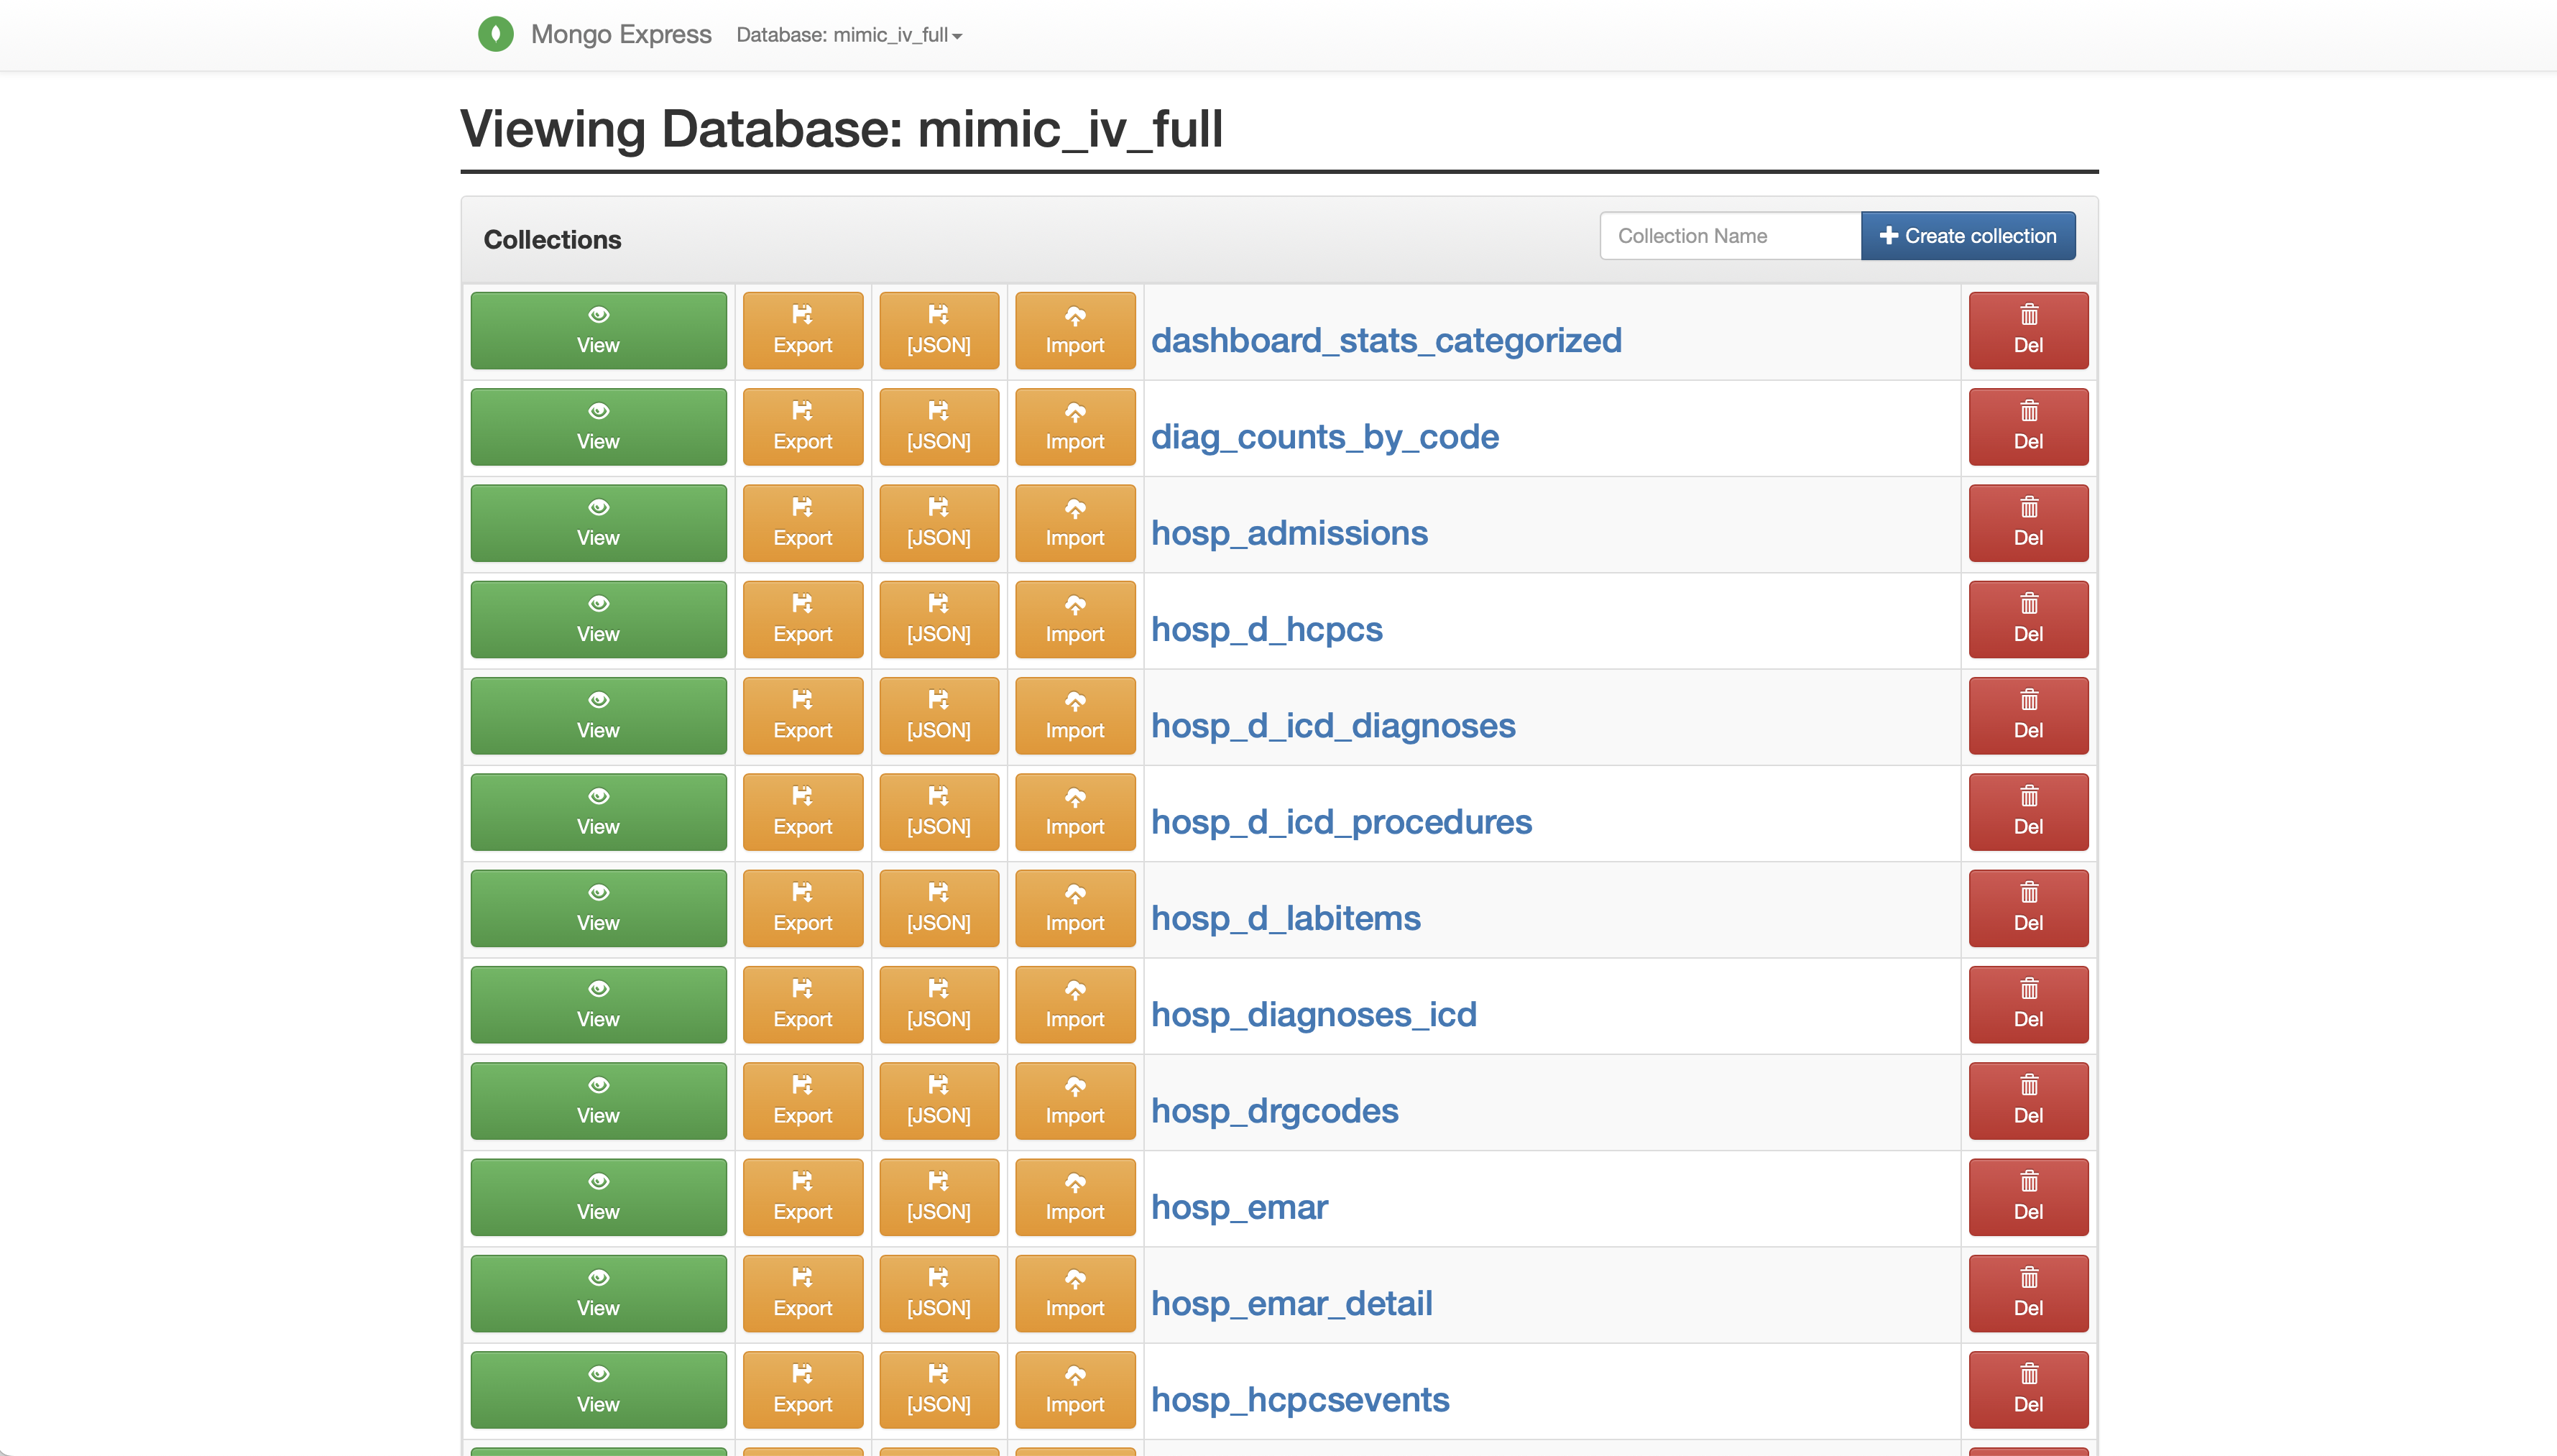
\includegraphics[width=1\textwidth]{imagenes/screenshot2.png}}
%  \caption{Captura de pantalla de Mongo Express}
%  \label{fig:screenshot2}
%\end{figure}


\subsection{API RESTful}

La API que obtiene, procesa y sirve los datos está construida sobre FastAPI \cite{fastapi}, un framework moderno que combina alto rendimiento con una sintaxis intuitiva y generación automática de documentación. Para separar responsabilidades, el código se estructura de la siguiente forma:

\begin{itemize}
\item \textbf{Capa de datos:} El módulo \texttt{db/mongo.py} encapsula la conexión a MongoDB y proporciona funciones de utilidad.
\item \textbf{Capa de rutas:} Organizadas por funcionalidad en el directorio \texttt{routes/}, incluyen endpoints para pacientes, dashboard, gráficos y chat.
\item \textbf{Capa de aplicación:} El archivo principal \texttt{main.py} configura la aplicación, middleware CORS y el enrutamiento.
\end{itemize}

Utilizamos Uvicorn como servidor ASGI (Asynchronous Server Gateway Interface) que escuchará las peticiones a los endpoints.

\subsubsection{ASGI y Uvicorn}

ASGI (Asynchronous Server Gateway Interface) representa la evolución natural de WSGI hacia aplicaciones Python asíncronas. A diferencia de WSGI, que maneja solicitudes de forma síncrona una por una, ASGI permite el procesamiento concurrente de múltiples solicitudes en un solo hilo mediante programación basada en eventos. Esta arquitectura resulta fundamental para aplicaciones web de alto rendimiento que requieren comunicación en tiempo real, como las funcionalidades de chat implementadas en esta plataforma.

La especificación ASGI define tres componentes principales en cada aplicación: el \textit{scope} (diccionario con información de la conexión y protocolo), \textit{receive} (callable asíncrono que recibe eventos) y \textit{send} (callable asíncrono que envía respuestas). Esta estructura permite soportar múltiples protocolos como HTTP, WebSocket y HTTP/2 de manera unificada.

Uvicorn es el servidor ASGI seleccionado para ejecutar la aplicación FastAPI. Sus principales ventajas incluyen alto rendimiento (construido sobre uvloop y httptools), eficiencia de recursos (aproximadamente 20MB de memoria base por worker) y capacidad de manejar gran número de conexiones concurrentes. El comando utilizado para ejecutar el servidor es:

\begin{verbatim}
python -m uvicorn app.main:app --reload --port 8088 --host 0.0.0.0
\end{verbatim}

\subsubsection{Endpoints implementados}

La API está estructurada modularmente mediante routers de FastAPI, organizados por funcionalidad:

\textbf{Endpoints de pacientes (\texttt{/api/patients}):}
\begin{itemize}
\item \texttt{GET /api/patients/\{subject\_id\}}: Obtiene información completa de un paciente específico mediante múltiples agregaciones MongoDB que incluyen datos demográficos, historial de ingresos, diagnósticos con descripciones ICD, procedimientos y eventos de laboratorio agrupados por ingreso.
\item \texttt{HEAD /api/patients/\{subject\_id\}/exists}: Verificación rápida de existencia de paciente (HTTP 200/404).
\item \texttt{GET /api/patients/}: Lista los primeros pacientes disponibles del dataset demo.
\end{itemize}

\textbf{Endpoints del dashboard (\texttt{/api/dashboard}):}
\begin{itemize}
\item \texttt{GET /api/dashboard/stats}: Obtiene estadísticas categorizadas pre-calculadas desde la colección \texttt{dashboard\_stats\_categorized} para máximo rendimiento, organizadas en cinco categorías: Demographics \& Admissions, Diagnoses \& Procedures, ICU Care, Lab \& Medications, y Hospital Flows.
\end{itemize}

\textbf{Endpoints de gráficos (\texttt{/api/charts}):}
\begin{itemize}
\item \texttt{GET /api/charts/admission-heatmap}: Genera datos para mapas de calor de ingresos hospitalarios con opciones de filtrado y vistas horarias/mensuales.
\item \texttt{GET /api/charts/age-distribution}: Distribución de pacientes por edad y género para pirámides poblacionales.
\item \texttt{GET /api/charts/icu-stay-duration}: Duración promedio de estancias en UCI por unidad.
\item \texttt{GET /api/charts/diagnosis-icicle}: Datos para diagramas icicle de diagnósticos categorizados.
\item \texttt{GET /api/charts/medications-sunburst}: Visualización sunburst de medicamentos prescritos por vía.
\item \texttt{GET /api/charts/hospital-transfers-chord}: Datos para diagramas chord de transferencias hospitalarias.
\end{itemize}

\textbf{Endpoints de inteligencia artificial:}
\begin{itemize}
\item \texttt{POST /chat/}: Interfaz de chat con streaming response que integra OpenAI GPT-5 con herramientas MCP para consultas en lenguaje natural sobre datos MIMIC-IV.
\item \texttt{POST /api/summary/patient}: Genera resúmenes clínicos automatizados utilizando OpenAI GPT-4.1.
\end{itemize}

\textbf{Endpoints de monitoreo:}
\begin{itemize}
\item \texttt{GET /health}: Verificación de estado del servidor.
\item \texttt{GET /}: Endpoint raíz con información básica de la API.
\end{itemize}

La API incluye middleware CORS configurado para permitir peticiones desde cualquier origen durante el desarrollo, y implementa una función \texttt{clean\_data()} que elimina valores NaN, null e infinitos de las respuestas, garantizando datos válidos para el frontend.

\subsection{Inteligencia Artificial}

La integración de inteligencia artificial en esta plataforma se fundamenta en la utilización de grandes modelos de lenguaje (LLMs) para facilitar la consulta y análisis de datos clínicos en lenguaje natural. Esta aproximación permite que usuarios sin conocimientos técnicos avanzados puedan extraer información valiosa de la base de datos MIMIC-IV mediante conversaciones naturales, eliminando la barrera técnica que tradicionalmente requería conocimientos de SQL o programación.

Para este proyecto se ha elegido trabajar con los modelos de texto de OpenAI, específicamente GPT-4.1, accedido mediante su API oficial para Python. Este modelo presentado por OpenAI en abril de 2025, representa una evolución significativa respecto a sus predecesores. Cuenta con una ventana de contexto ampliada de hasta 1 millón de tokens, superando significativamente los 128.000 tokens de modelos previos como GPT-4o, pero también modelos nuevos como GPT-5, que tiene una ventana de 400.000 tokens. Esta capacidad expandida permite procesar y analizar grandes volúmenes de información médica en una sola interacción, facilitando el análisis de múltiples registros clínicos, documentos extensos y conversaciones prolongadas sin perder coherencia ni relevancia contextual, y es principalmente ese el motivo de su elección.

\subsubsection{Model Context Protocol (MCP)}

Una de las innovaciones técnicas más relevantes incorporadas en este proyecto es la implementación del Model Context Protocol (MCP), un estándar abierto desarrollado por Anthropic y presentado en noviembre de 2024 \cite{AnthropicMCP2024}. MCP surge como respuesta a uno de los principales desafíos en el desarrollo de sistemas de inteligencia artificial: la integración estandarizada y segura entre modelos de lenguaje de gran tamaño y fuentes de datos externas.


Tradicionalmente, la conexión entre modelos de IA y bases de datos requería el desarrollo de integraciones personalizadas para cada caso específico. Técnicas como RAG (Retrieval-Augmented Generation), aunque efectivas para enriquecer las respuestas de los modelos con información externa, demandaban implementaciones ad-hoc para cada fuente de datos. Esta aproximación resultaba en arquitecturas complejas, propensas a errores y difíciles de mantener. Cada nueva fuente de datos o herramienta externa requería desarrollo personalizado, generando fragmentación tecnológica y duplicación de esfuerzos. MCP aborda estos problemas proporcionando una interfaz universal que estandariza la comunicación entre sistemas de IA y recursos externos, incluyendo bases de datos, APIs, sistemas de archivos y herramientas especializadas.


MCP opera bajo una arquitectura cliente-servidor compuesta por tres componentes principales \cite{mcp_arch}:

\begin{itemize}
\item \textbf{MCP Host:} La aplicación principal que requiere acceso a datos externos, como una interfaz de chat impulsada por IA o un entorno de desarrollo integrado.
\item \textbf{MCP Client:} Un componente que mantiene una conexión dedicada con un servidor MCP específico y obtiene contexto de dicho servidor para que lo utilice el host MCP. Cada cliente mantiene una relación uno-a-uno con su servidor correspondiente.
\item \textbf{MCP Server:} Programas especializados que se conectan a fuentes de datos específicas y exponen funcionalidades a través del protocolo MCP estandarizado.
\end{itemize}

El flujo de comunicación se inicia cuando el modelo de IA necesita acceder a información externa. El anfitrión envía una solicitud al cliente MCP, quien la encamina al servidor correspondiente. Este último procesa la petición, accede a los datos requeridos y devuelve la información siguiendo el protocolo establecido. Esta arquitectura modular garantiza que los modelos de IA tengan acceso a contexto actualizado y relevante sin comprometer la seguridad o integridad de los datos subyacentes.

En el contexto de esta plataforma, se ha desarrollado un servidor MCP especializado para interactuar con la base de datos MIMIC-IV almacenada en MongoDB. Para ello, se utilizó FastMCP \cite{fastmcp}, un framework Python diseñado específicamente para simplificar la creación de servidores que implementan el Model Context Protocol. Con esta herramienta, nuestra tarea únicamente se reduce a definir las herramientas a las que podrán acceder los LLMs. En nuestro caso, se han implementado las siguientes seis herramientas que permiten la interacción con la base de datos:

\begin{itemize}
\item \texttt{get\_schema}: Obtiene la estructura de cualquier colección MongoDB, permitiendo al modelo entender los campos disponibles y sus tipos de datos.
\item \texttt{find\_documents}: Realiza consultas directas sobre documentos específicos, aplicando filtros y limitaciones de resultados.
\item \texttt{aggregate\_data}: Ejecuta pipelines de agregación MongoDB para análisis complejos y cálculos estadísticos.
\item \texttt{count\_documents}: Proporciona conteos rápidos de documentos que cumplen criterios específicos.
\item \texttt{list\_collections}: Enumera todas las colecciones disponibles en la base de datos.
\item \texttt{get\_indexes}: Obtiene información sobre índices de rendimiento de las colecciones.
\end{itemize}


\begin{figure}[H]
  \centering
  \fbox{
\includegraphics[width=0.4\textwidth]{imagenes/fastmpc.png}}
  %
\includegraphics[width=0.4\textwidth]{imagenes/fastmpc.png}
  \caption{Logo del framework FastMCP.}
  \label{fig:fastmcp}
\end{figure}



El servidor MCP se integra con el sistema principal montándose en el endpoint \texttt{/mcp} de la API principal, mientras que el cliente de chat utiliza OpenAI Response API configurado con herramientas MCP que apuntan al servidor local. Esta arquitectura permite que el modelo GPT-4.1 acceda directamente a los datos clínicos de MIMIC-IV de forma estructurada y segura.

%La adopción de MCP en esta plataforma aporta múltiples beneficios técnicos y funcionales:

%\textbf{Estandarización:} Elimina la necesidad de desarrollar interfaces propietarias para cada tipo de consulta, reduciendo significativamente la complejidad del código y el tiempo de desarrollo.

%\textbf{Escalabilidad:} La arquitectura modular facilita la incorporación de nuevas fuentes de datos o herramientas sin modificar el núcleo del sistema de IA.

%\textbf{Seguridad:} Cada servidor MCP gestiona sus propios permisos y controles de acceso, proporcionando una capa adicional de seguridad sin comprometer la funcionalidad.

%\textbf{Rendimiento:} Al proporcionar acceso directo y estructurado a los datos relevantes, el modelo puede generar respuestas más precisas y contextualizadas con menor latencia.

%\textbf{Interoperabilidad:} Al seguir un estándar abierto, el sistema puede integrarse con otras herramientas y plataformas que adopten MCP, facilitando la colaboración y extensibilidad.

%La implementación de MCP representa así un paso hacia la madurez tecnológica en el campo de la integración de sistemas de IA con infraestructuras de datos complejas, posicionando este proyecto como un ejemplo práctico de las mejores prácticas emergentes en el desarrollo de aplicaciones sanitarias inteligentes.

(... hablar sobre tema legal de proteccion de datos... todaviia no se si se puede...)

\subsection{Despliegue}

Para la implementación del backend, era necesario considerar los importantes requisitos de hardware que impone el conjunto de datos MIMIC-IV. Específicamente, se requería almacenamiento considerable para albergar los múltiples gigabytes de información clínica, así como múltiples núcleos de procesamiento para gestionar eficientemente las consultas paralelas a la base de datos y las peticiones simultáneas de la API.

En lugar de alquilar un VPS (Virtual Private Server) con estas especificaciones técnicas, lo que representaría un coste económico significativo para un proyecto académico, se optó por utilizar un servidor personal disponible. Este servidor ejecuta Proxmox VE \cite{proxmox}, un hipervisor de código abierto basado en Debian que combina virtualización de máquinas (KVM) y contenedores (LXC), proporcionando una plataforma completa para la gestión de infraestructura virtualizada.


\begin{figure}[H]
  \centering
  \fbox{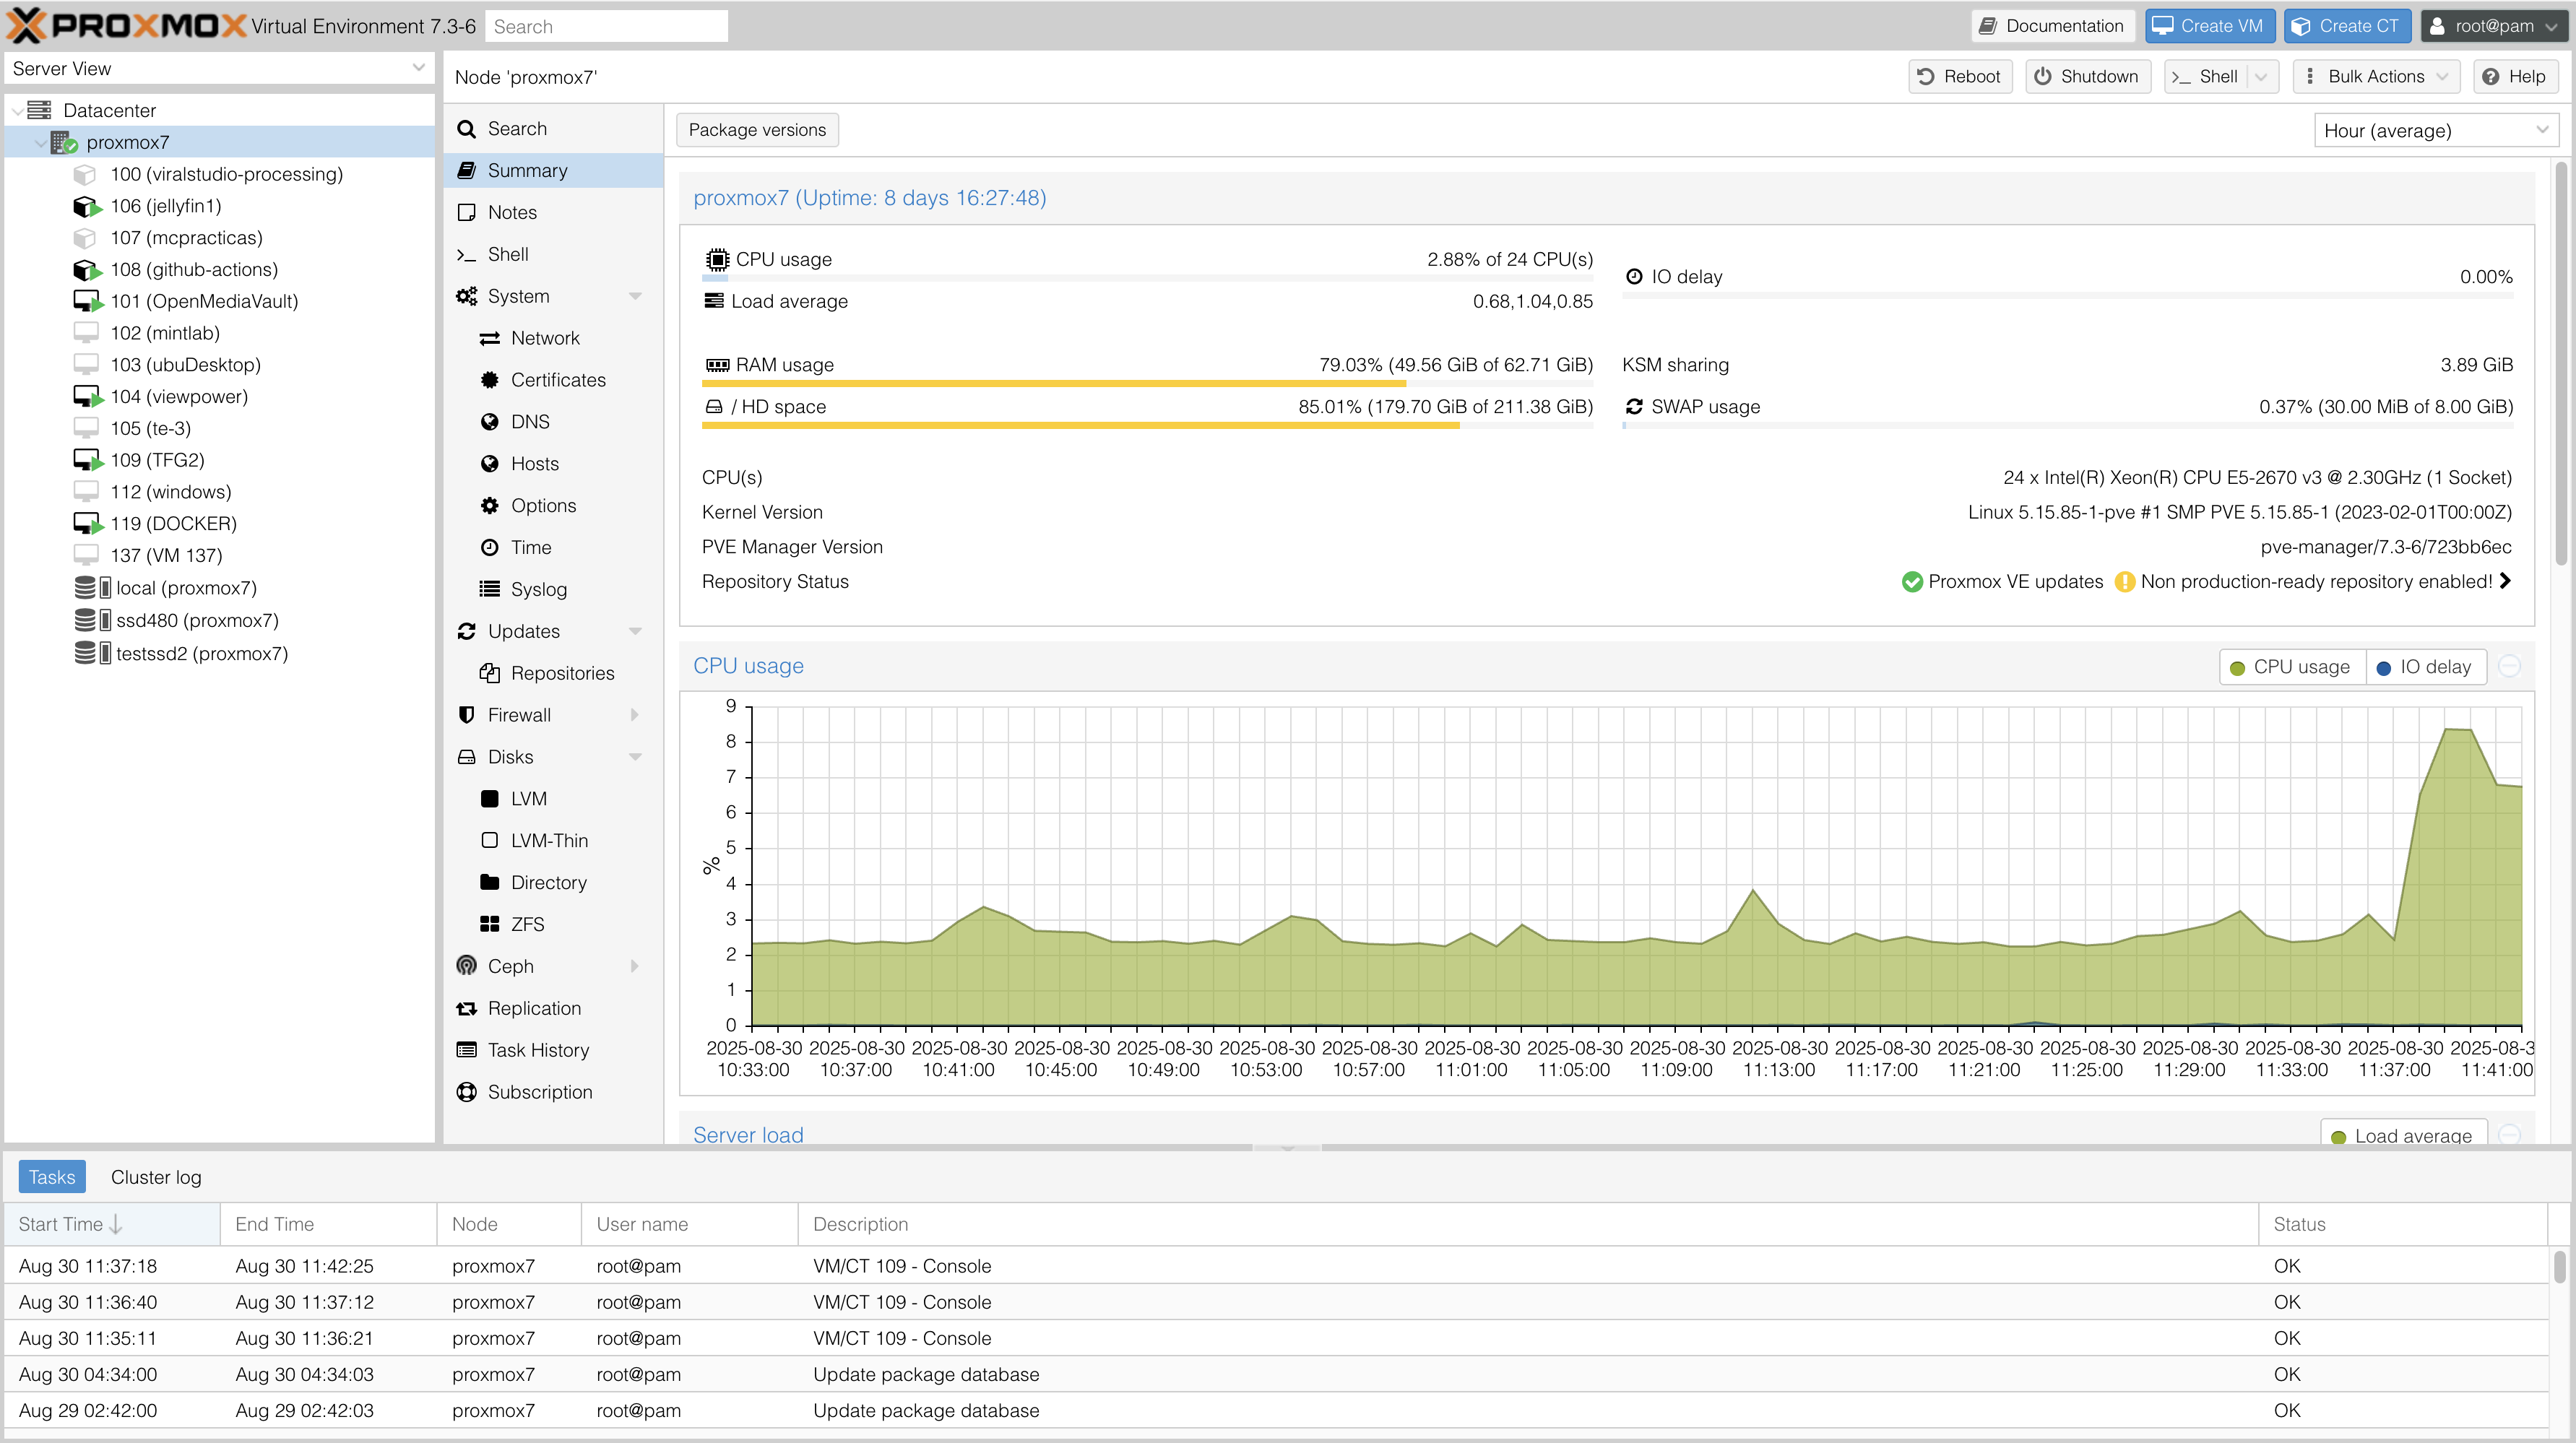
\includegraphics[width=1\textwidth]{imagenes/proxmox2.png}}
  %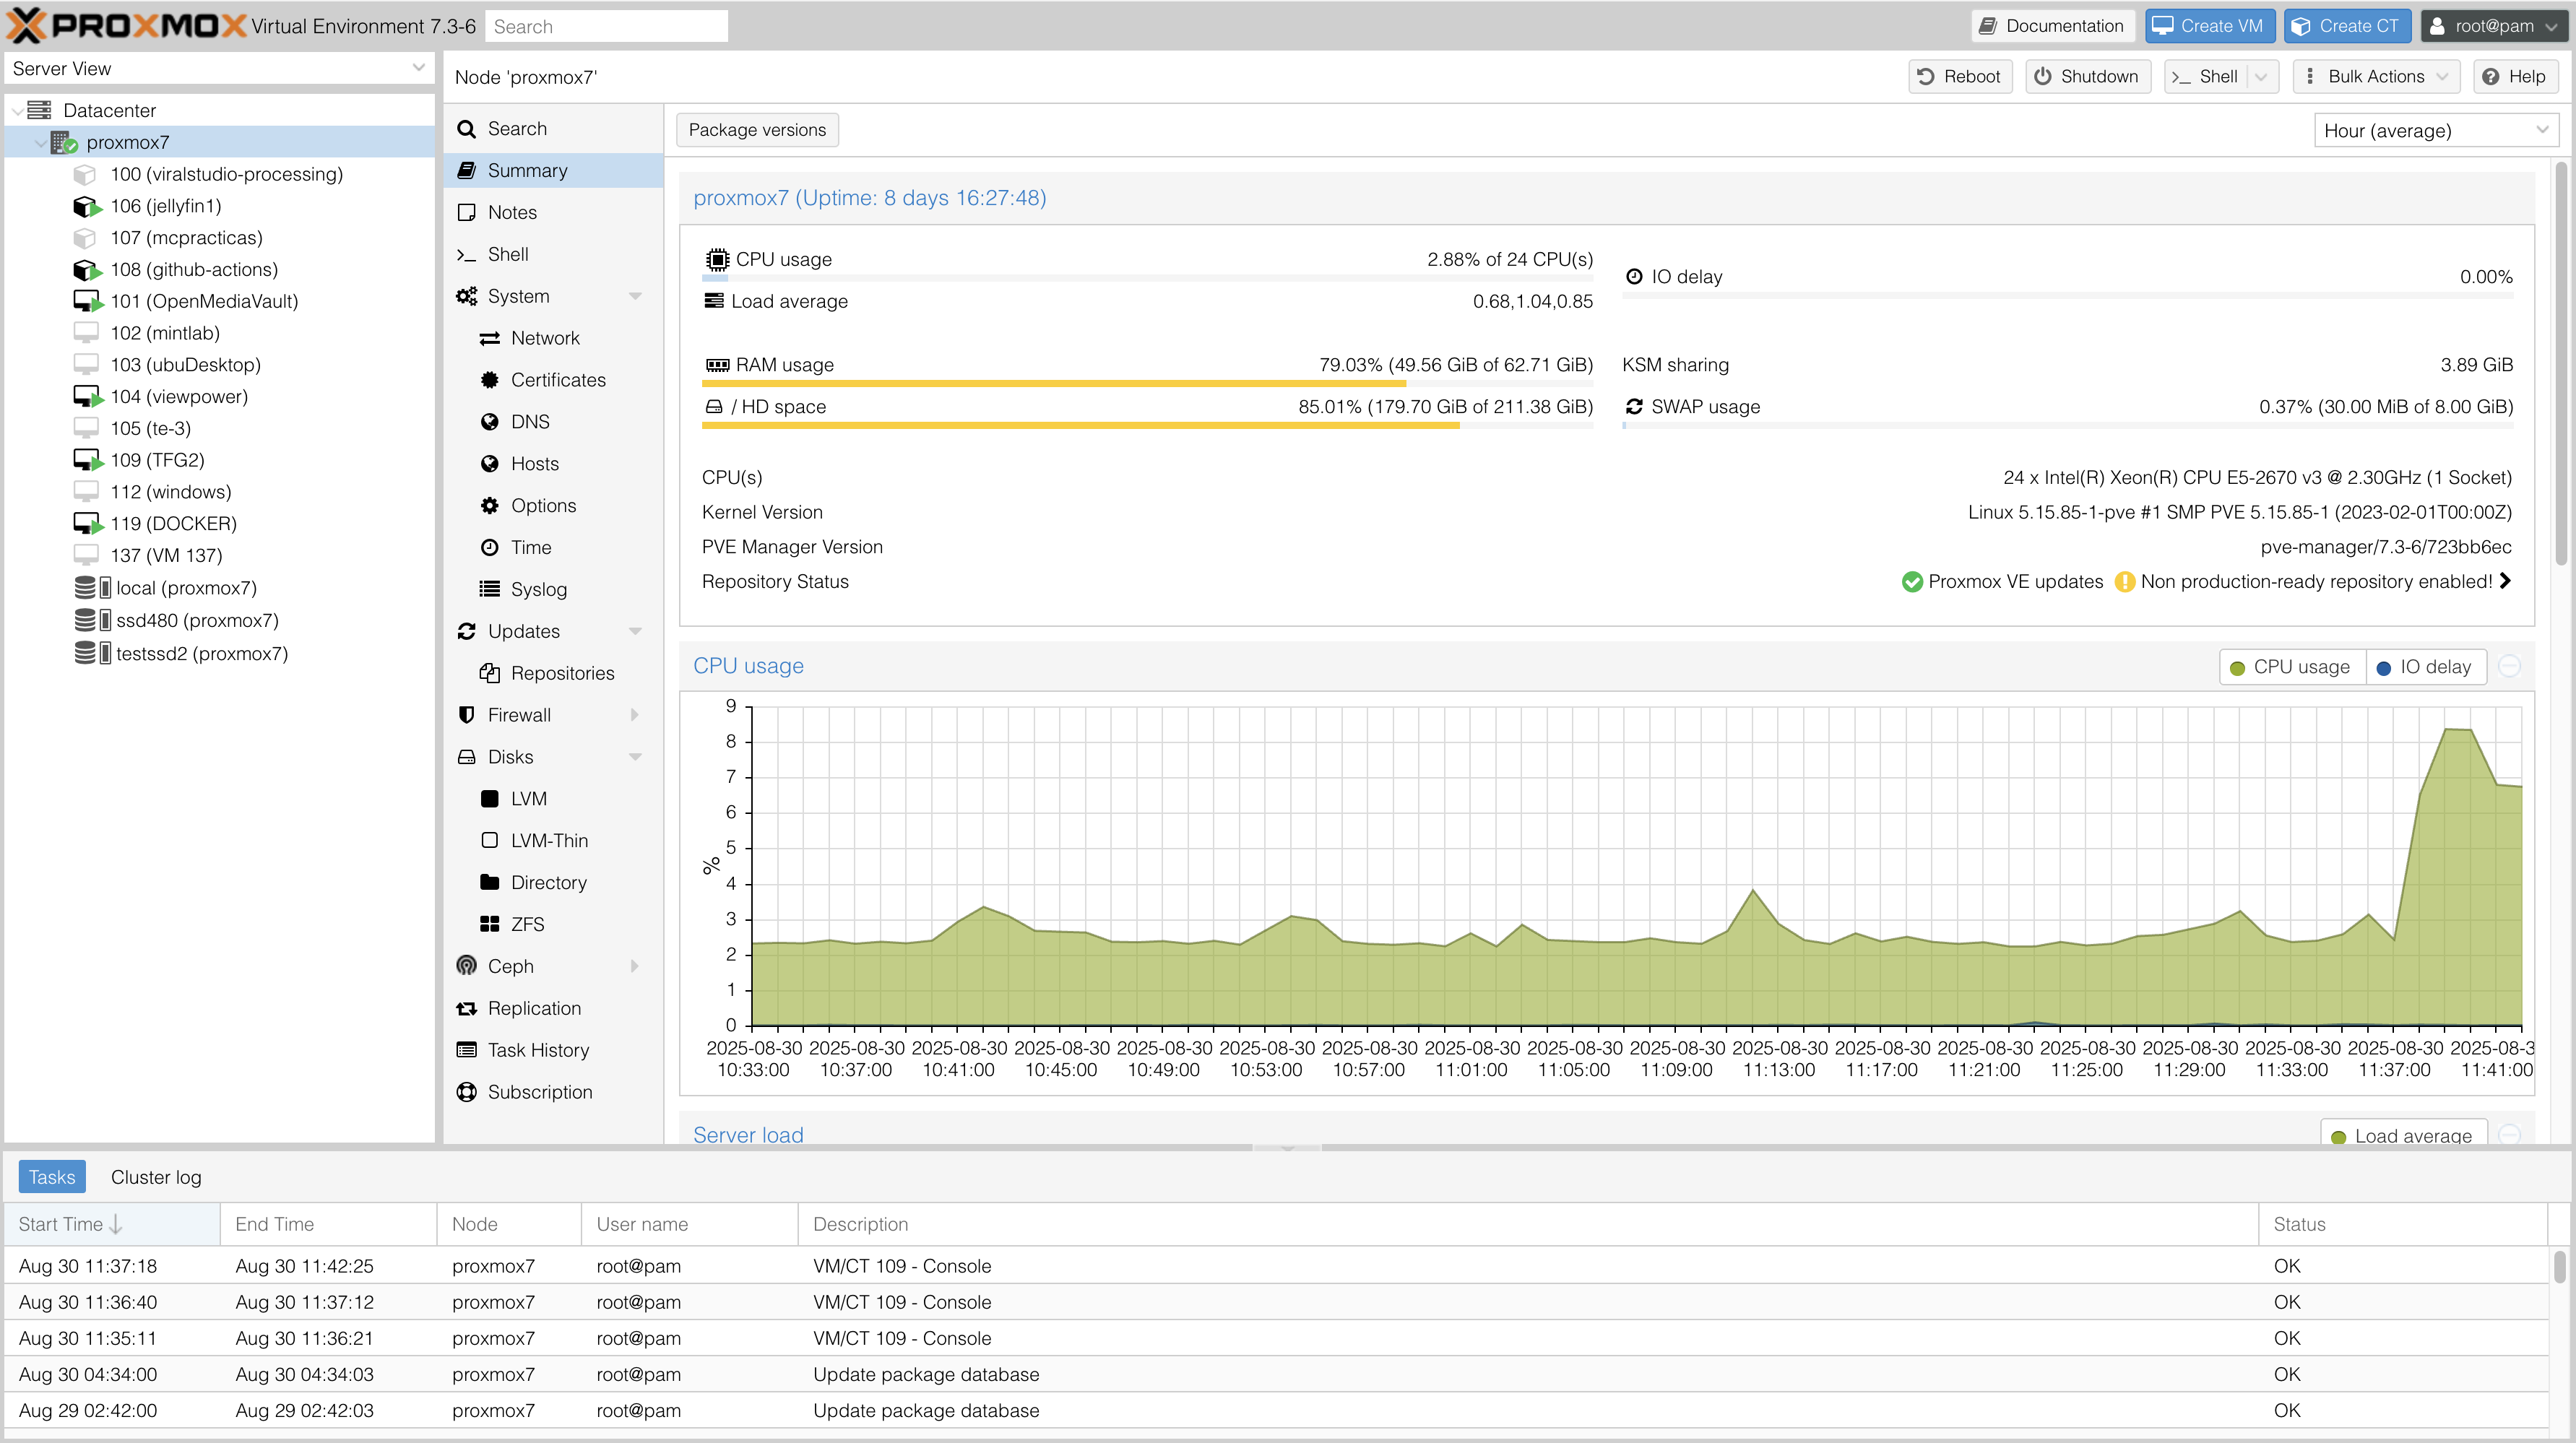
\includegraphics[width=1\textwidth]{imagenes/proxmox2.png}
  \caption{Captura de pantalla de la interfaz de Proxmox.}
  \label{fig:proxmox2}
\end{figure}



Se creó una máquina virtual con Ubuntu 24.04 Desktop como sistema operativo guest. Los recursos asignados a esta máquina virtual se fueron incrementando iterativamente según las necesidades observadas durante las pruebas de carga y la importación de datos. La configuración final establecida fue de 10 núcleos de CPU, 26 GB de memoria RAM y 128 GB de almacenamiento SSD, especificaciones que proporcionaron el rendimiento adecuado para gestionar tanto la base de datos MongoDB como la API.

Una vez que tanto la base de datos como la API funcionaban correctamente en el entorno local, era necesario desplegarlos para permitir el acceso público desde el frontend. Para esta tarea se utilizó Cloudflare Tunnels \cite{cloudflaretunnels}, que permite exponer servicios locales a Internet sin abrir puertos en el firewall ni configurar redirección de puertos. Cloudflare \cite{cloudflare} es una empresa que actúa como intermediario proporcionando servicios de CDN, DNS y seguridad web entre los usuarios finales y los servidores.

El despliegue se realizó mediante un contenedor Docker adicional que ejecuta el cliente \texttt{cloudflared}, estableciendo una conexión cifrada entre el servidor local y la infraestructura de Cloudflare. Esta implementación permite que la API sea accesible públicamente a través de un dominio o subdominio de nuestra elección, en nuestro caso \texttt{https://tfg-api.angeloyo.com}, proporcionando automáticamente certificados SSL/TLS, protección DDoS y optimizaciones de red.

Las principales ventajas de esta aproximación son su simplicidad y que mantiene el servidor completamente privado, ofreciendo una URL HTTPS estable consumible desde cualquier ubicación. Sin embargo, esta solución, aunque perfecta para el contexto de este TFG, no sería adecuada para entornos de producción profesionales donde se requerirían arquitecturas más robustas con balanceadores de carga, alta disponibilidad y redundancia geográfica.  


\begin{figure}[H]
  \centering
  \fbox{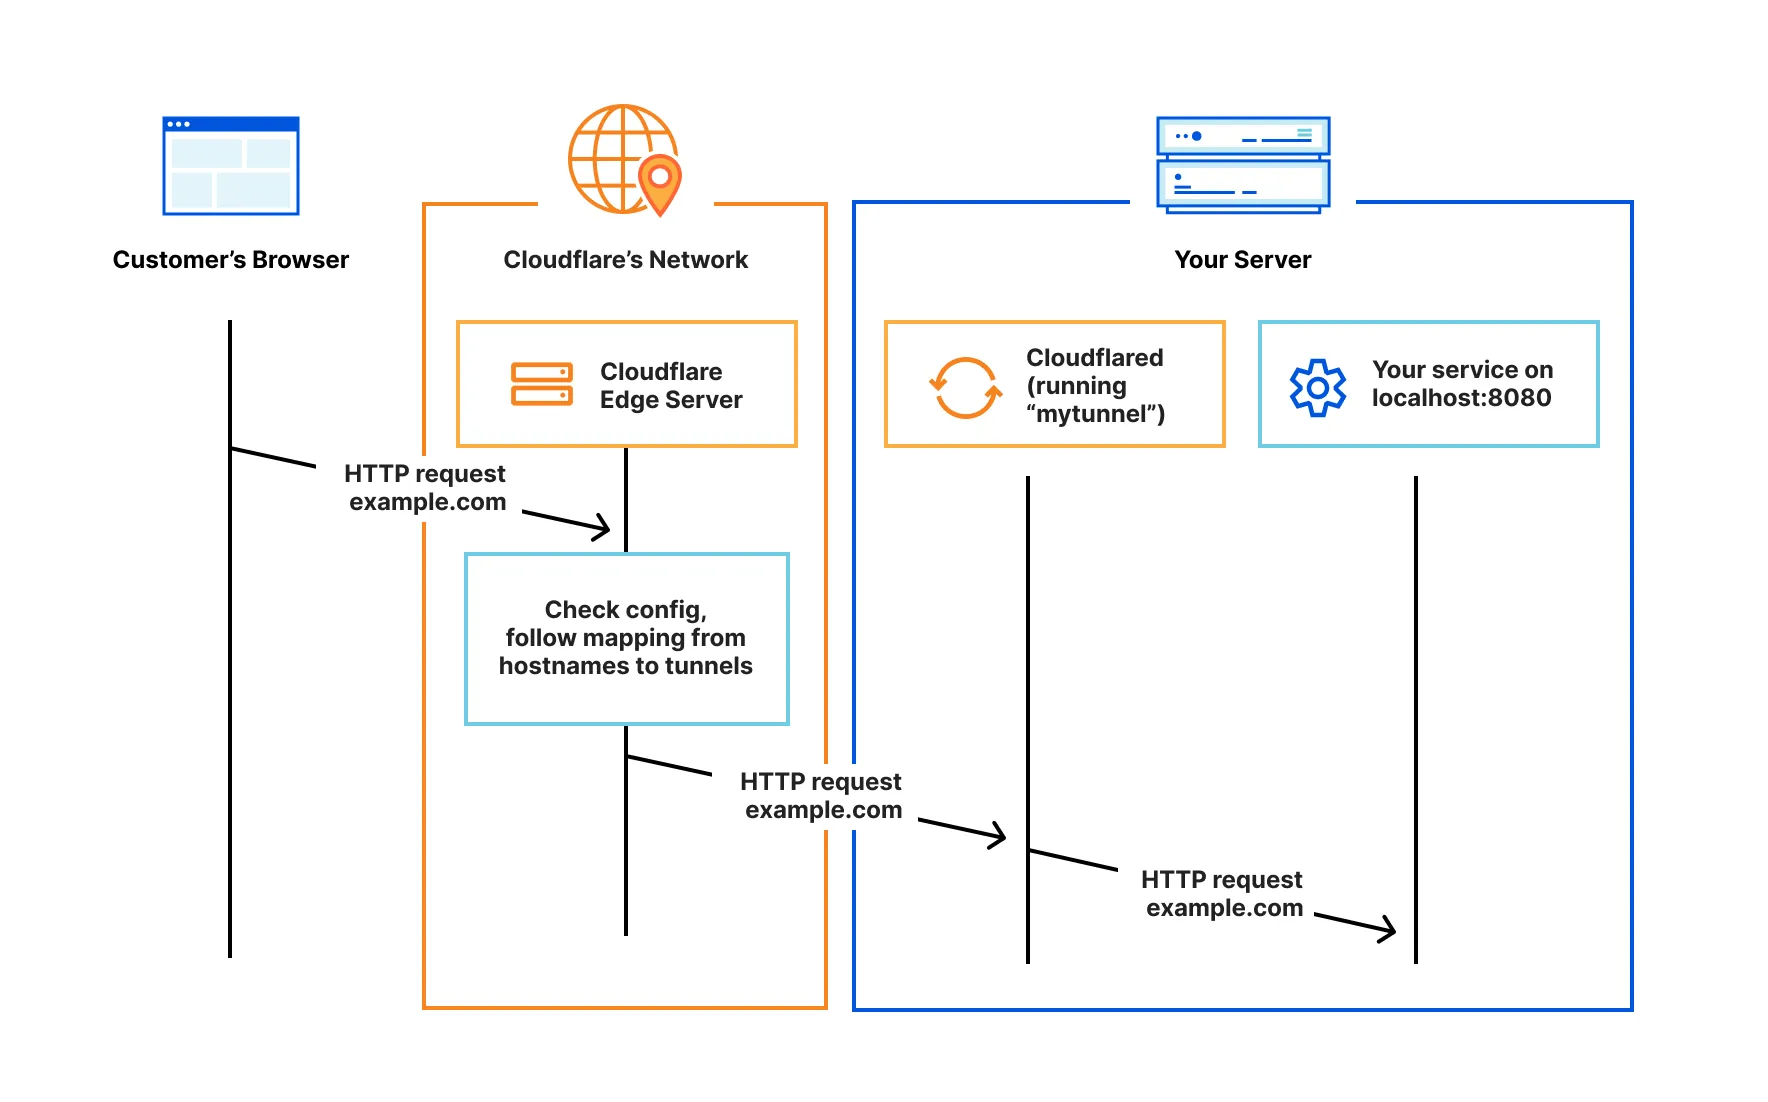
\includegraphics[width=1\textwidth]{imagenes/cloudflared.png}}
  %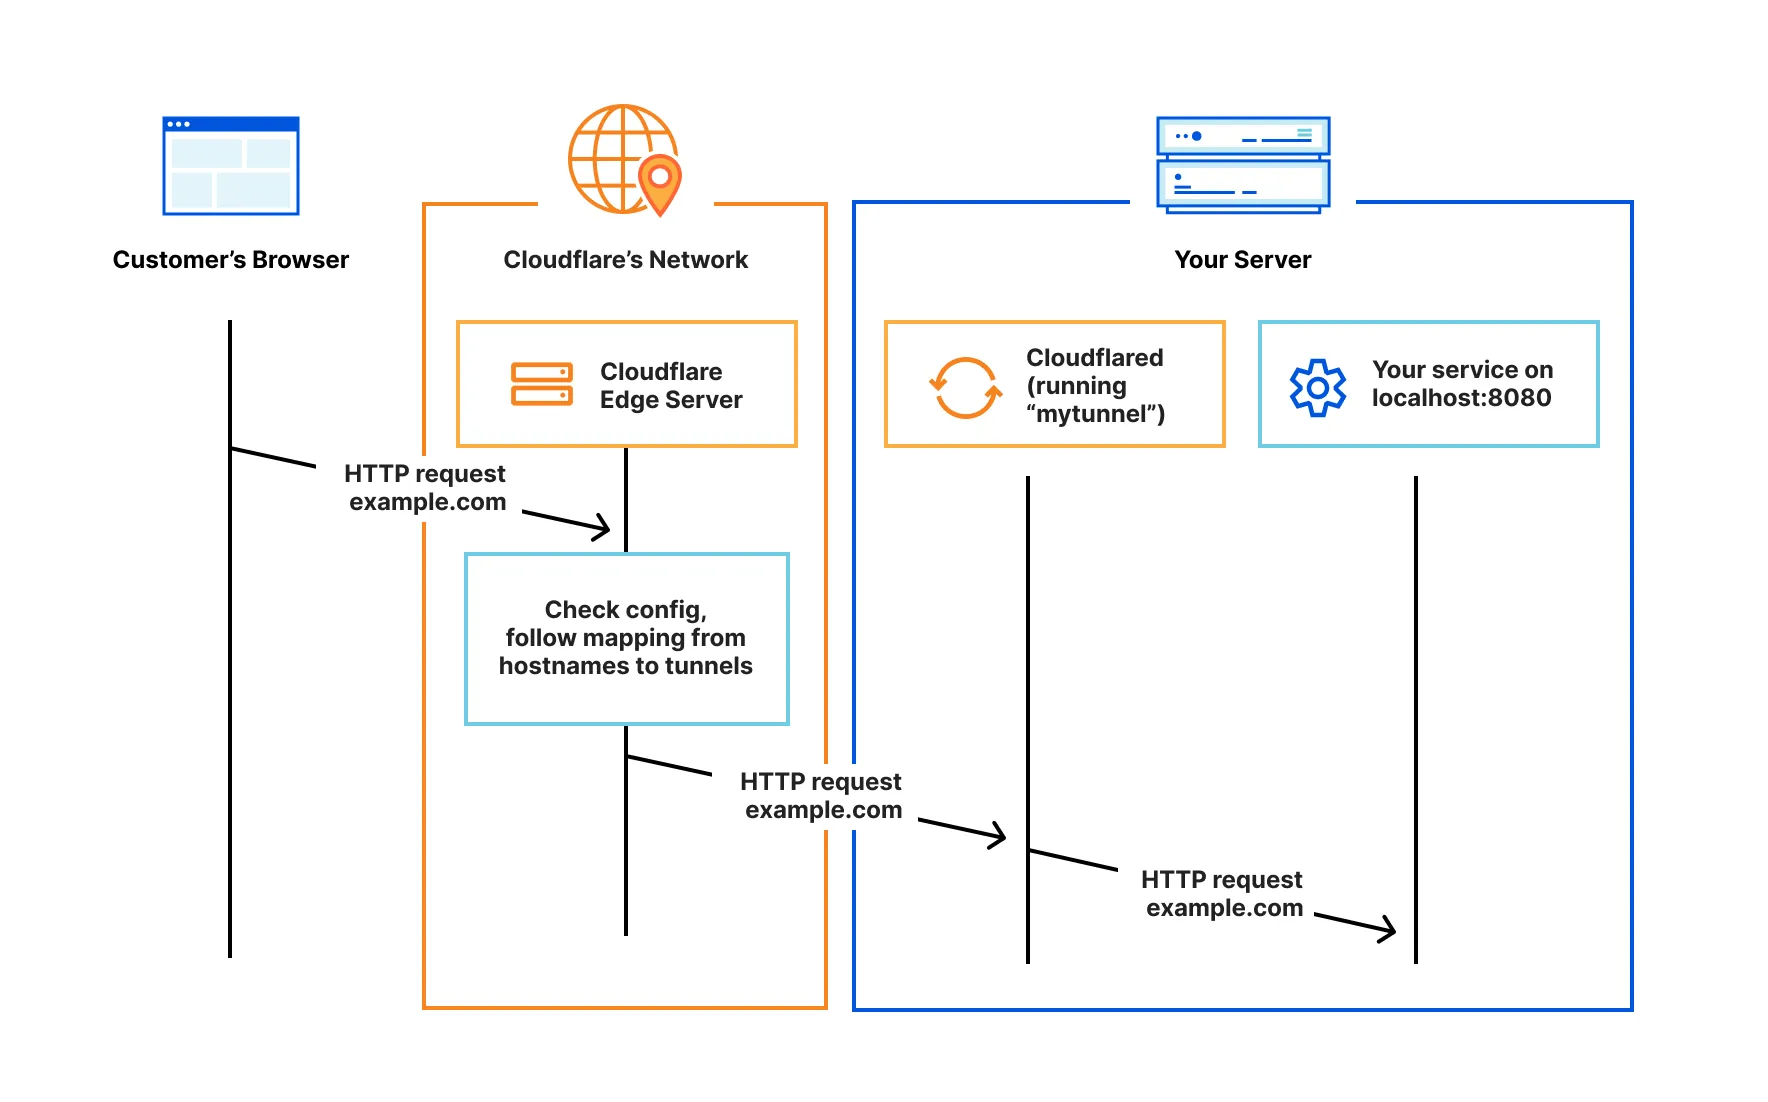
\includegraphics[width=1\textwidth]{imagenes/cloudflared.png}
  \caption{Esquema del funcionamiento de Cloudflare Tunnels \cite{cloudflaretunnels}.}
  \label{fig:cloudflared}
\end{figure}


\newpage
\section{Frontend}

%\subsection{Tecnologías}

El frontend está desarrollado utilizando Next.js 15 y TypeScript. Se aloja la web en Vercel por su extrema facilidad de uso, plan gratuito, auto-deploy desde GitHub, gran optimización y CDN global. La arquitectura se basa en componentes reutilizables y páginas especializadas que consumen la API del backend.



\subsection{Arquitectura de Componentes}

La estructura del frontend sigue las convenciones de Next.js con el nuevo App Router, organizando el código en:

\begin{itemize}
\item \textbf{Páginas:} Ubicadas en \texttt{src/app/}, incluyen la página principal, dashboard, búsqueda de pacientes, chat y visualizaciones específicas.
\item \textbf{Componentes:} En \texttt{src/components/}, contienen elementos reutilizables como el header, componentes de gráficos y elementos de UI.
\item \textbf{Hooks personalizados:} En \texttt{src/hooks/}, encapsulan lógica específica como el monitoreo de salud del backend.
\item \textbf{Tipos TypeScript:} En \texttt{src/types/}, definen las interfaces de datos para garantizar type safety.
\end{itemize}

Se utiliza Lucide React para iconografía consistente y Tailwind CSS para el diseño.

\subsection{Visualización de Datos}

Se ha implementado una estrategia progresiva para la visualización de datos, empleando dos librerías principales según la complejidad de cada caso. Para los gráficos más básicos se utiliza Observable Plot \cite{observableplot}, que ofrece soluciones preestablecidas y una integración sencilla. Cuando se requieren visualizaciones más complejas que demandan un control granular sobre el renderizado y la interactividad, se recurre a D3 \cite{d3}, también desarrollada por Observable, lo que permite adaptar los gráficos a necesidades avanzadas, sin salir del mismo ecosistema y estética.

Los componentes de visualización están diseñados como elementos autónomos que consumen datos de la API y manejan sus propios estados de carga y error. Esta aproximación facilita la reutilización y el testing individual de cada visualización.


\subsection{Páginas implementadas}

A continuación se detallan todas las páginas del Frontend que se han implementado. Se ha buscado una UI (User Interface) minimalista, limpia, sencilla y moderna.

\subsubsection{Página principal}

La página principal o ``home'' se ha buscado que sea muy sencilla, sólo se muestra el nombre dado a la plataforma, MIMIC-IV Analytics, junto a un pequeño subtítulo. 


\begin{figure}[H]
  \centering
  \fbox{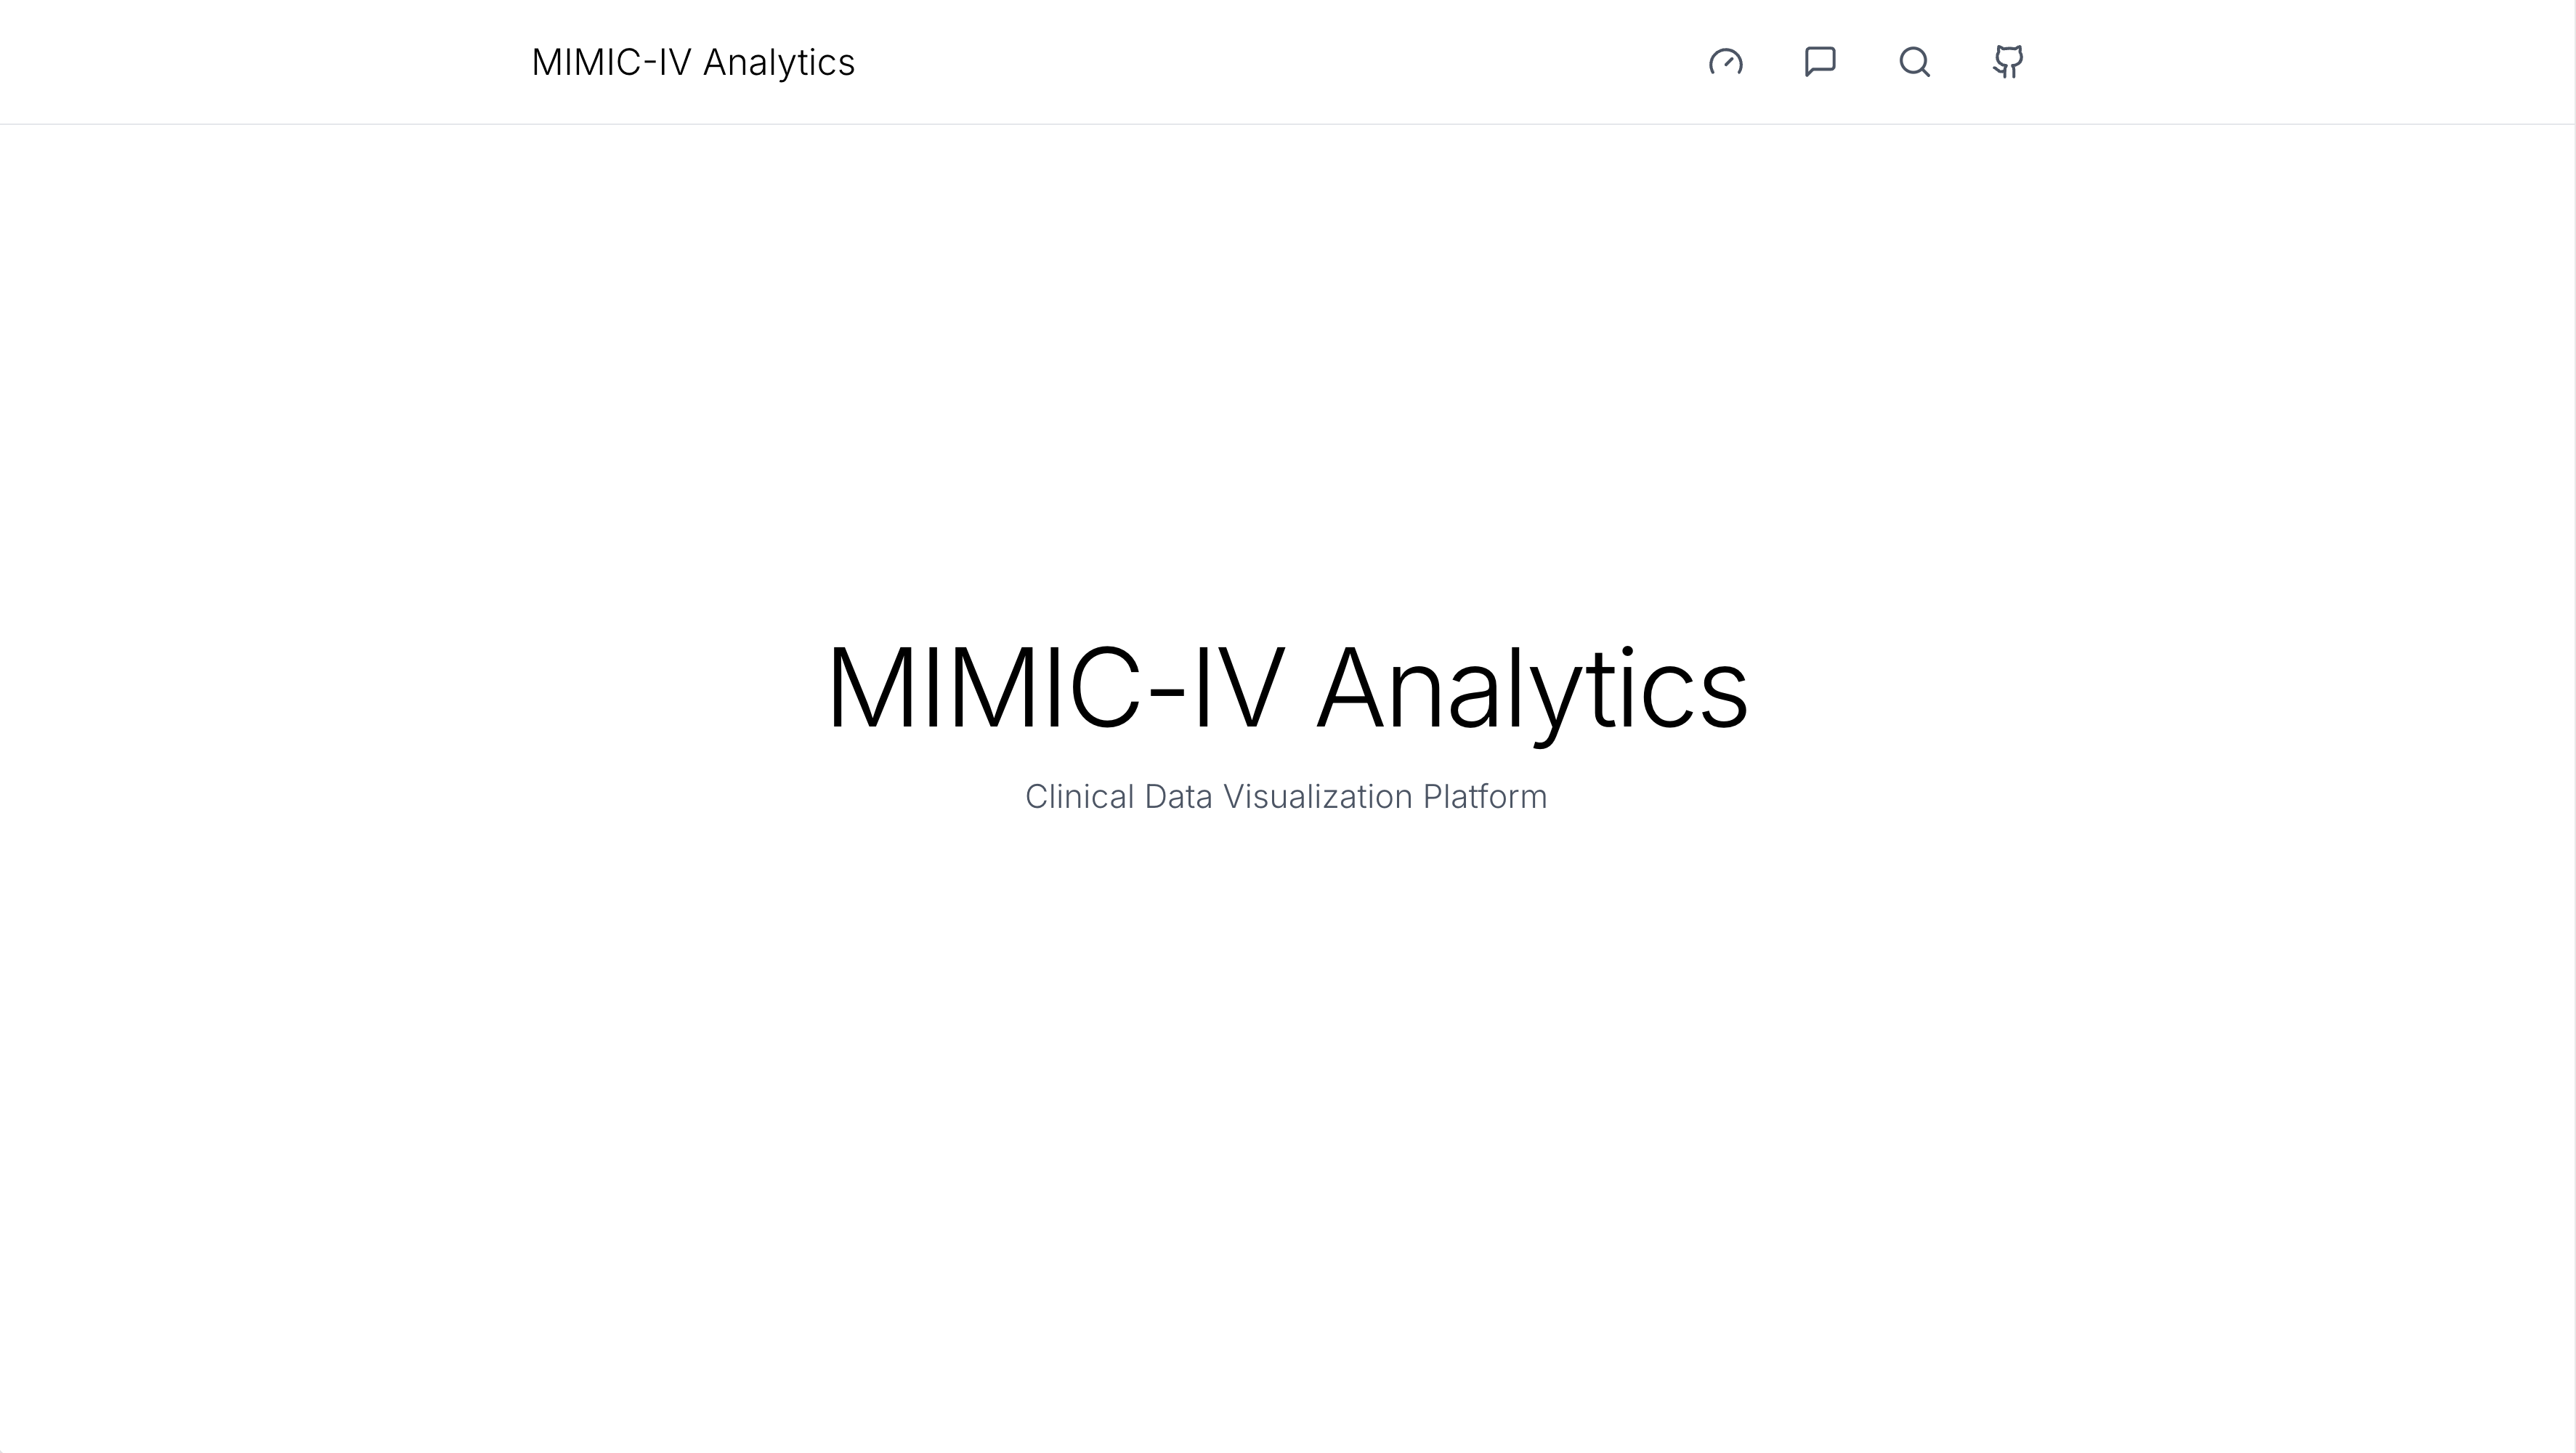
\includegraphics[width=1\textwidth]{imagenes/home.png}}
  \caption{Captura de pantalla de la página principal.}
  \label{fig:home}
\end{figure}


\subsubsection{Página del dashboard}

El objetivo de esta página es ofrecer al usuario una visión clara y accesible de las estadísticas más relevantes de la base de datos, seleccionadas por su importancia clínica. Para facilitar la interpretación y mejorar la experiencia de usuario, toda la información de MIMIC-IV se ha organizado en cinco grandes categorías: Demográficos y Admisiones, Cuidados Intensivos, Laboratorio y Medicamentos, Diagnósticos y Procedimientos, y Flujos Hospitalarios. En cada una de estas categorías se presentan tres indicadores estadísticos destacados, junto con enlaces a las visualizaciones asociadas. En total, se han implementado seis visualizaciones: dos para la categoría de Demográficos y Admisiones, y una para cada una de las categorías restantes.

En un entorno médico real e ideal, estos datos se actualizarían dinámicamente, permitiendo monitorizar de un vistazo los principales KPIs (Key Performance Indicators) y facilitando la toma de decisiones. Esta página sienta las bases para desarrollos futuros, en los que los profesionales sanitarios podrían filtrar los datos por periodos de tiempo, realizar comparativas o explorar tendencias, obteniendo así información relevante y actualizada sobre el estado del hospital. 


\begin{figure}[H]
  \centering
  \fbox{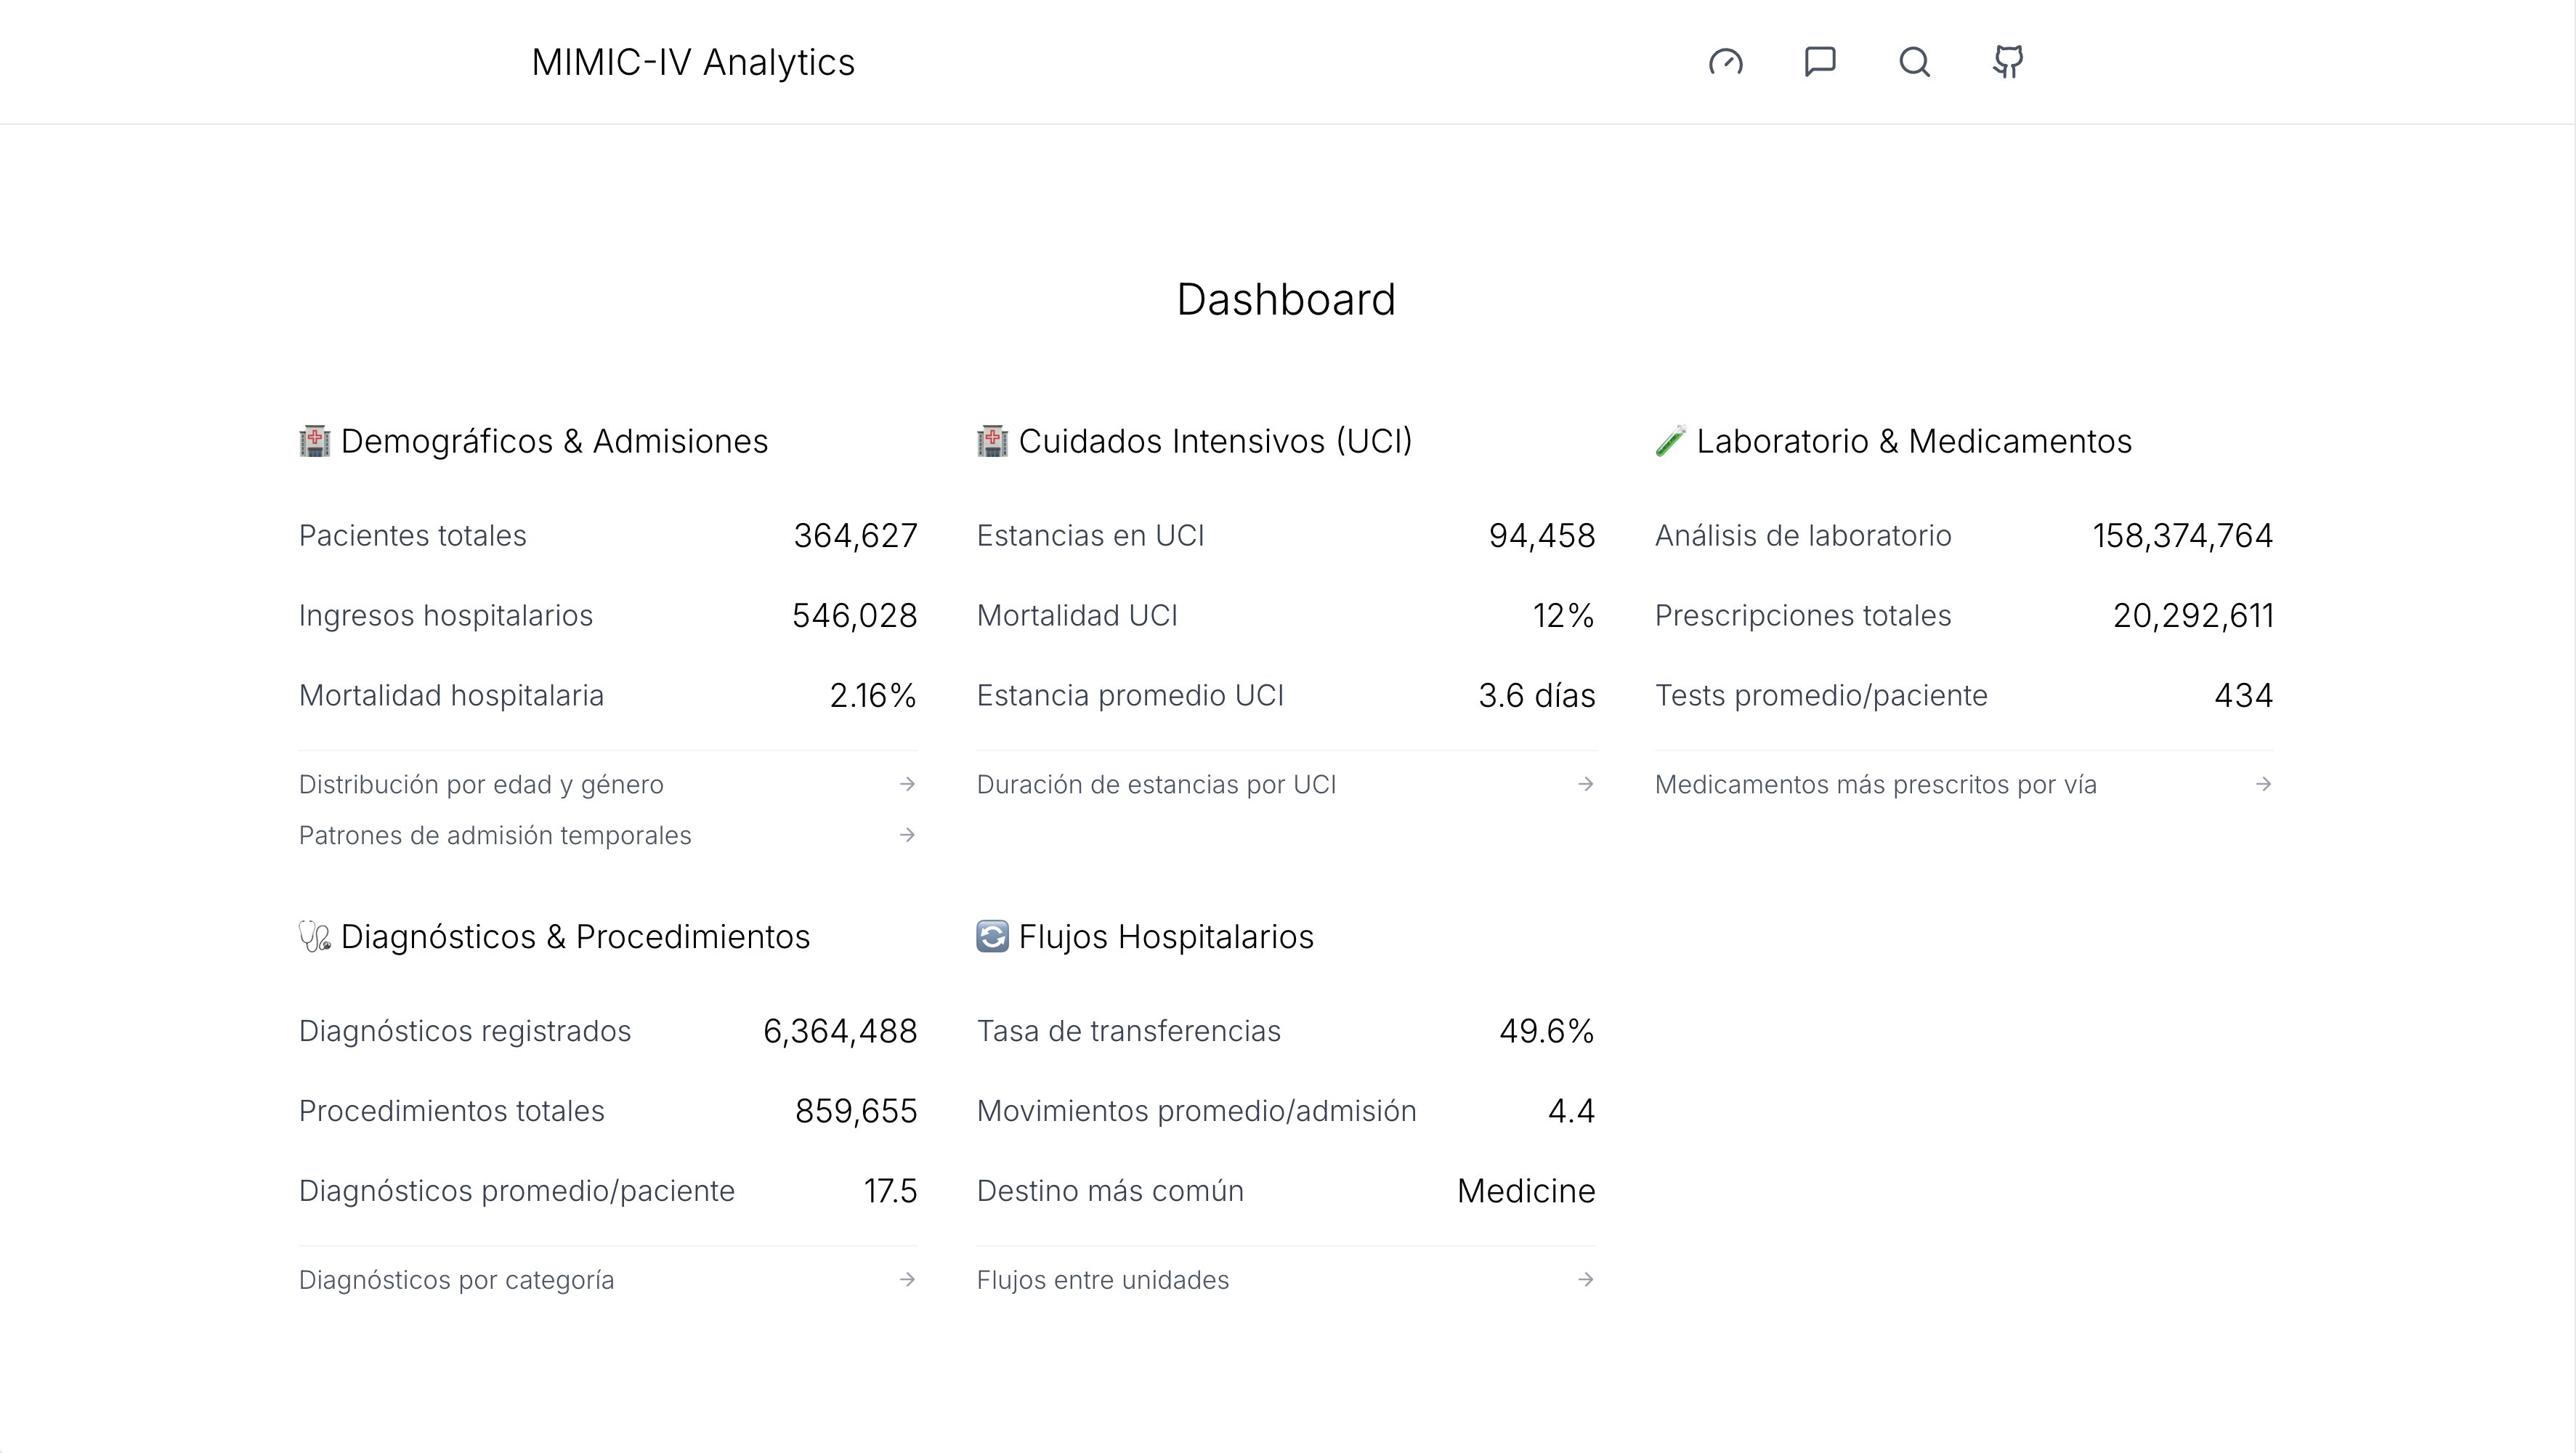
\includegraphics[width=1\textwidth]{imagenes/dash.png}}
  \caption{Captura de pantalla de la página del dashboard.}
  \label{fig:dash}
\end{figure}

\subsubsection{Página del chat}

Para la página del chat se sigue con la estética visual minimalista ya establecida, y se implementa la conexión con el backend, que ejecuta toda la lógica de comunicación entre el LLM, la base de datos gracias al protocolo MCP, y el frontend.

\begin{figure}[H]
  \centering
  \fbox{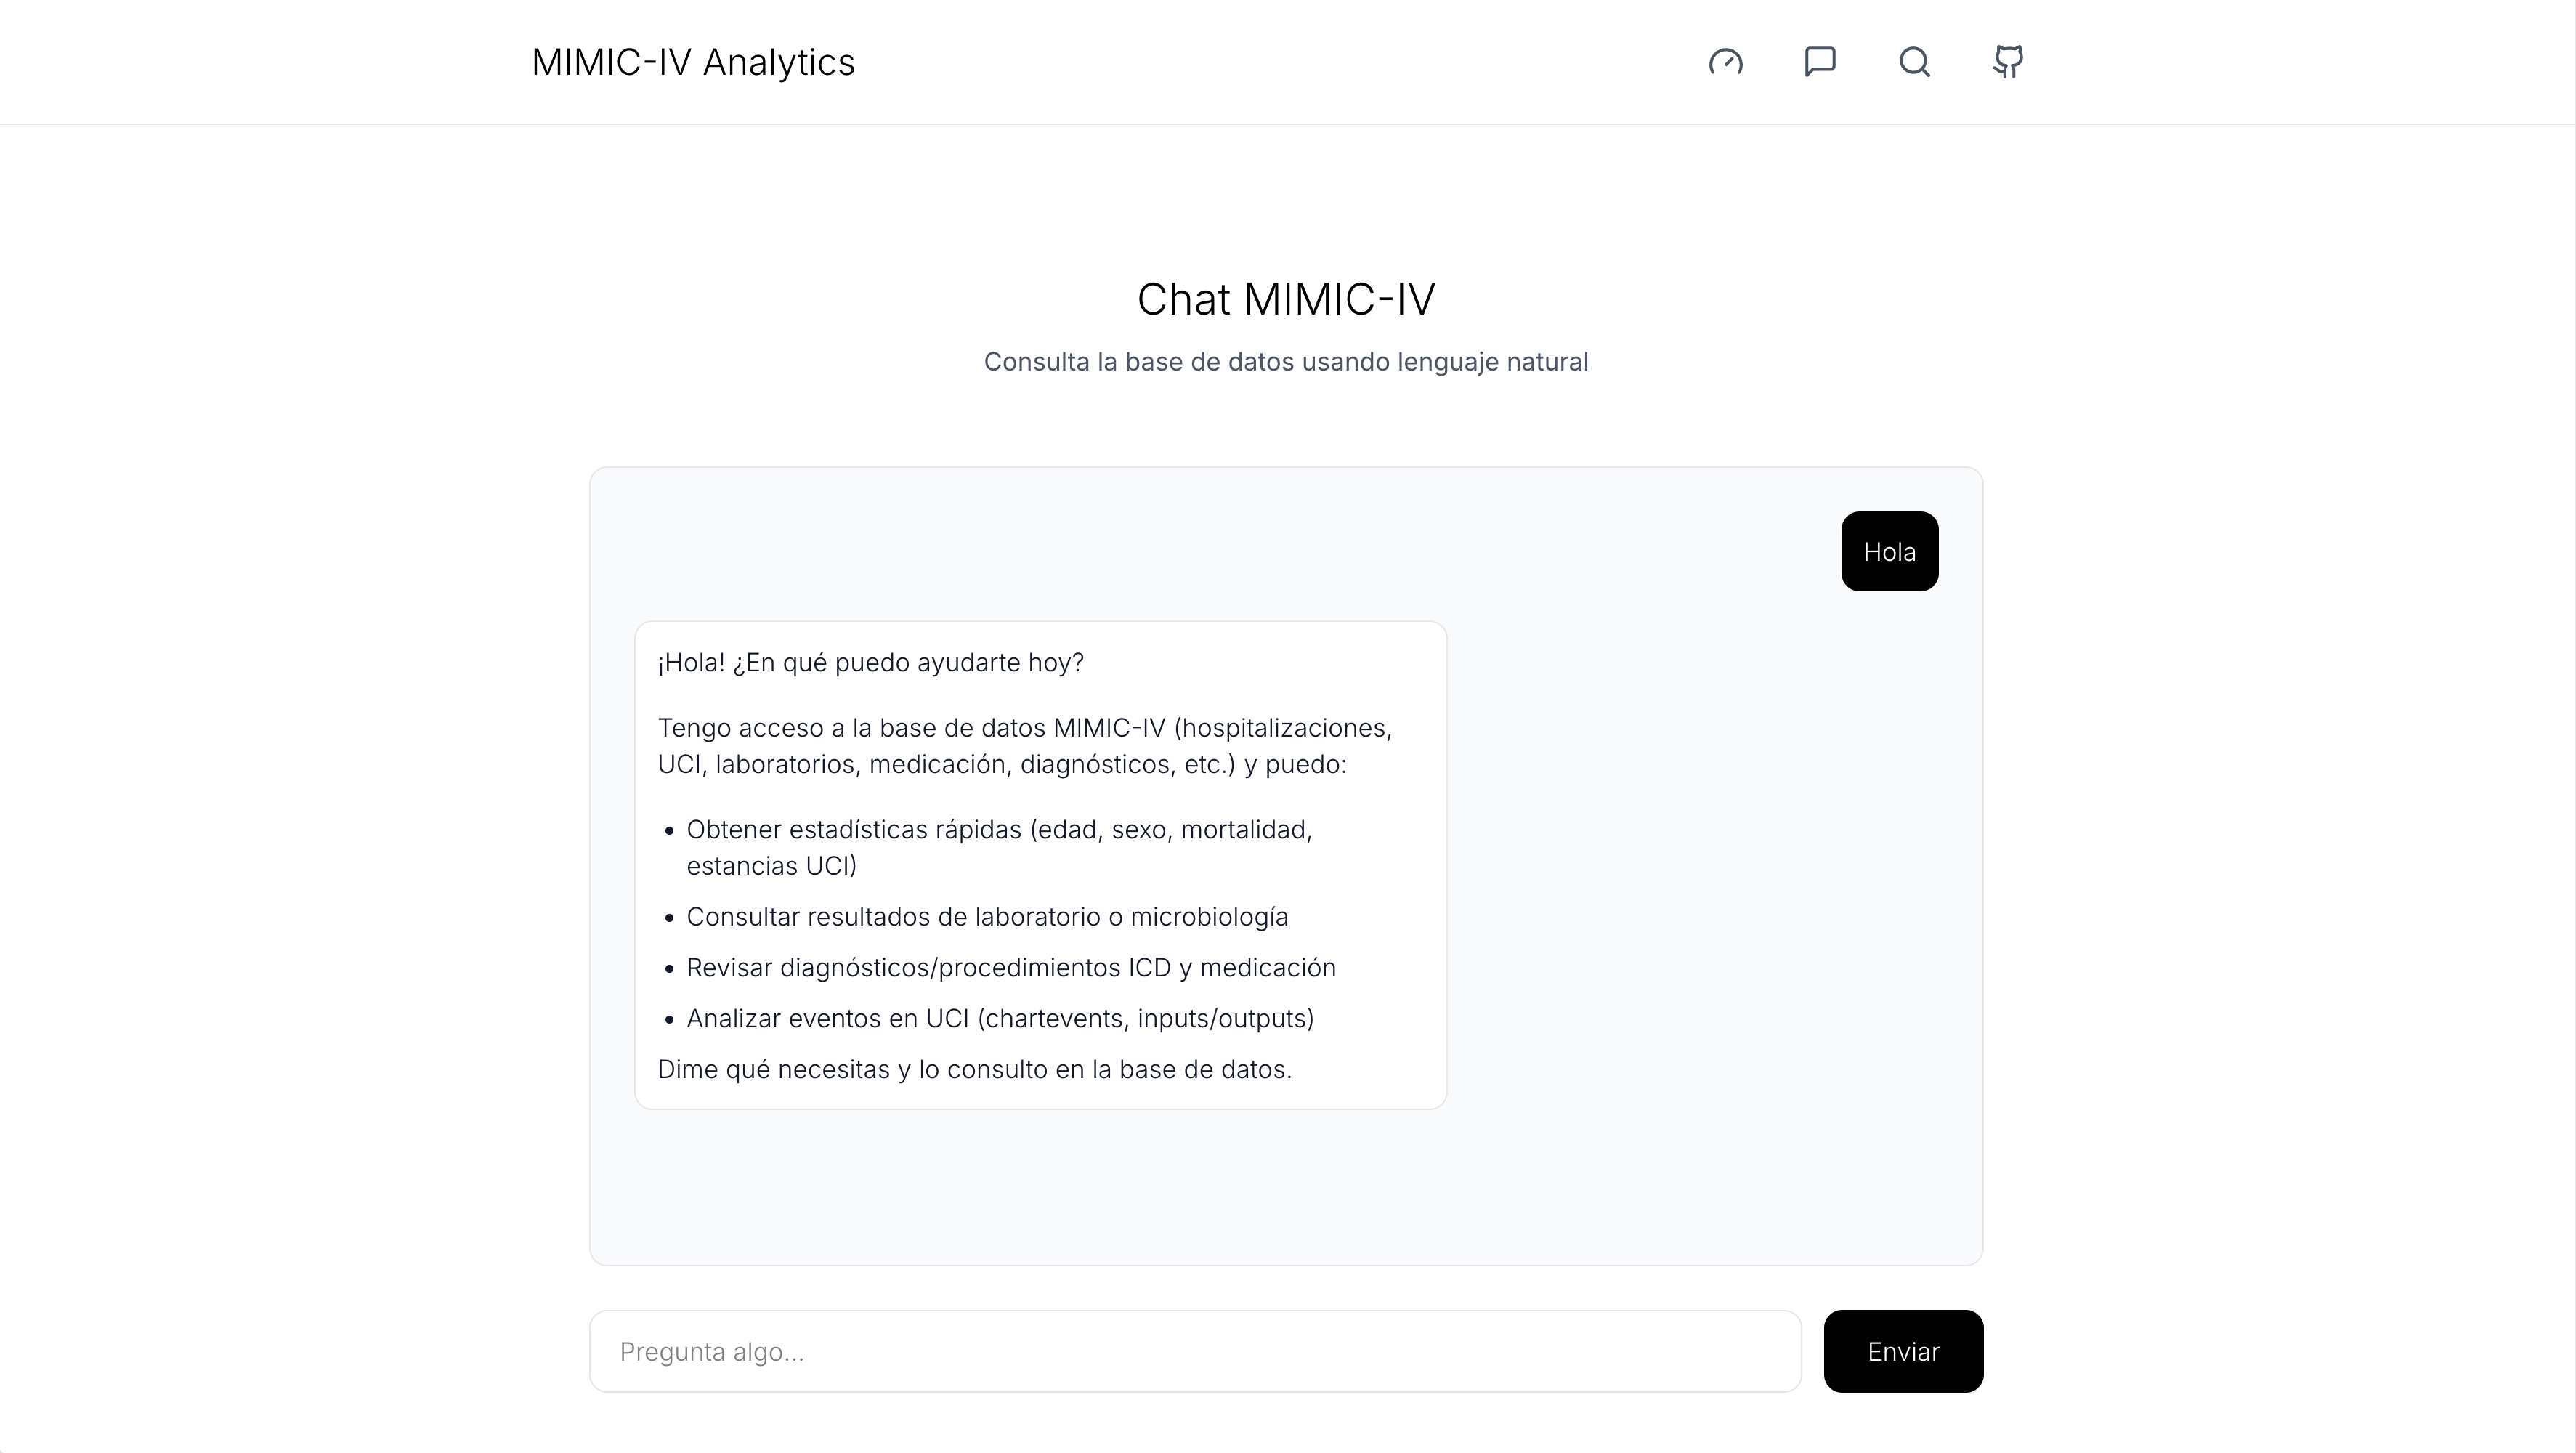
\includegraphics[width=1\textwidth]{imagenes/chat.png}}
  \caption{Captura de pantalla de la página del chat.}
  \label{fig:chat}
\end{figure}

\subsubsection{Página de búsqueda de pacientes}

Esta sencilla página nos permite comprobar la existencia de un paciente mediante su identificador único, mediante llamadas al endpoint del backend \texttt{/api/patients/\$\{id\}/exists}, y si es así (obtenemos status code 200 OK) entonces redirigimos a la página individual del paciente \texttt{/patient/\$\{id\}}. 

\begin{figure}[H]
  \centering
  \fbox{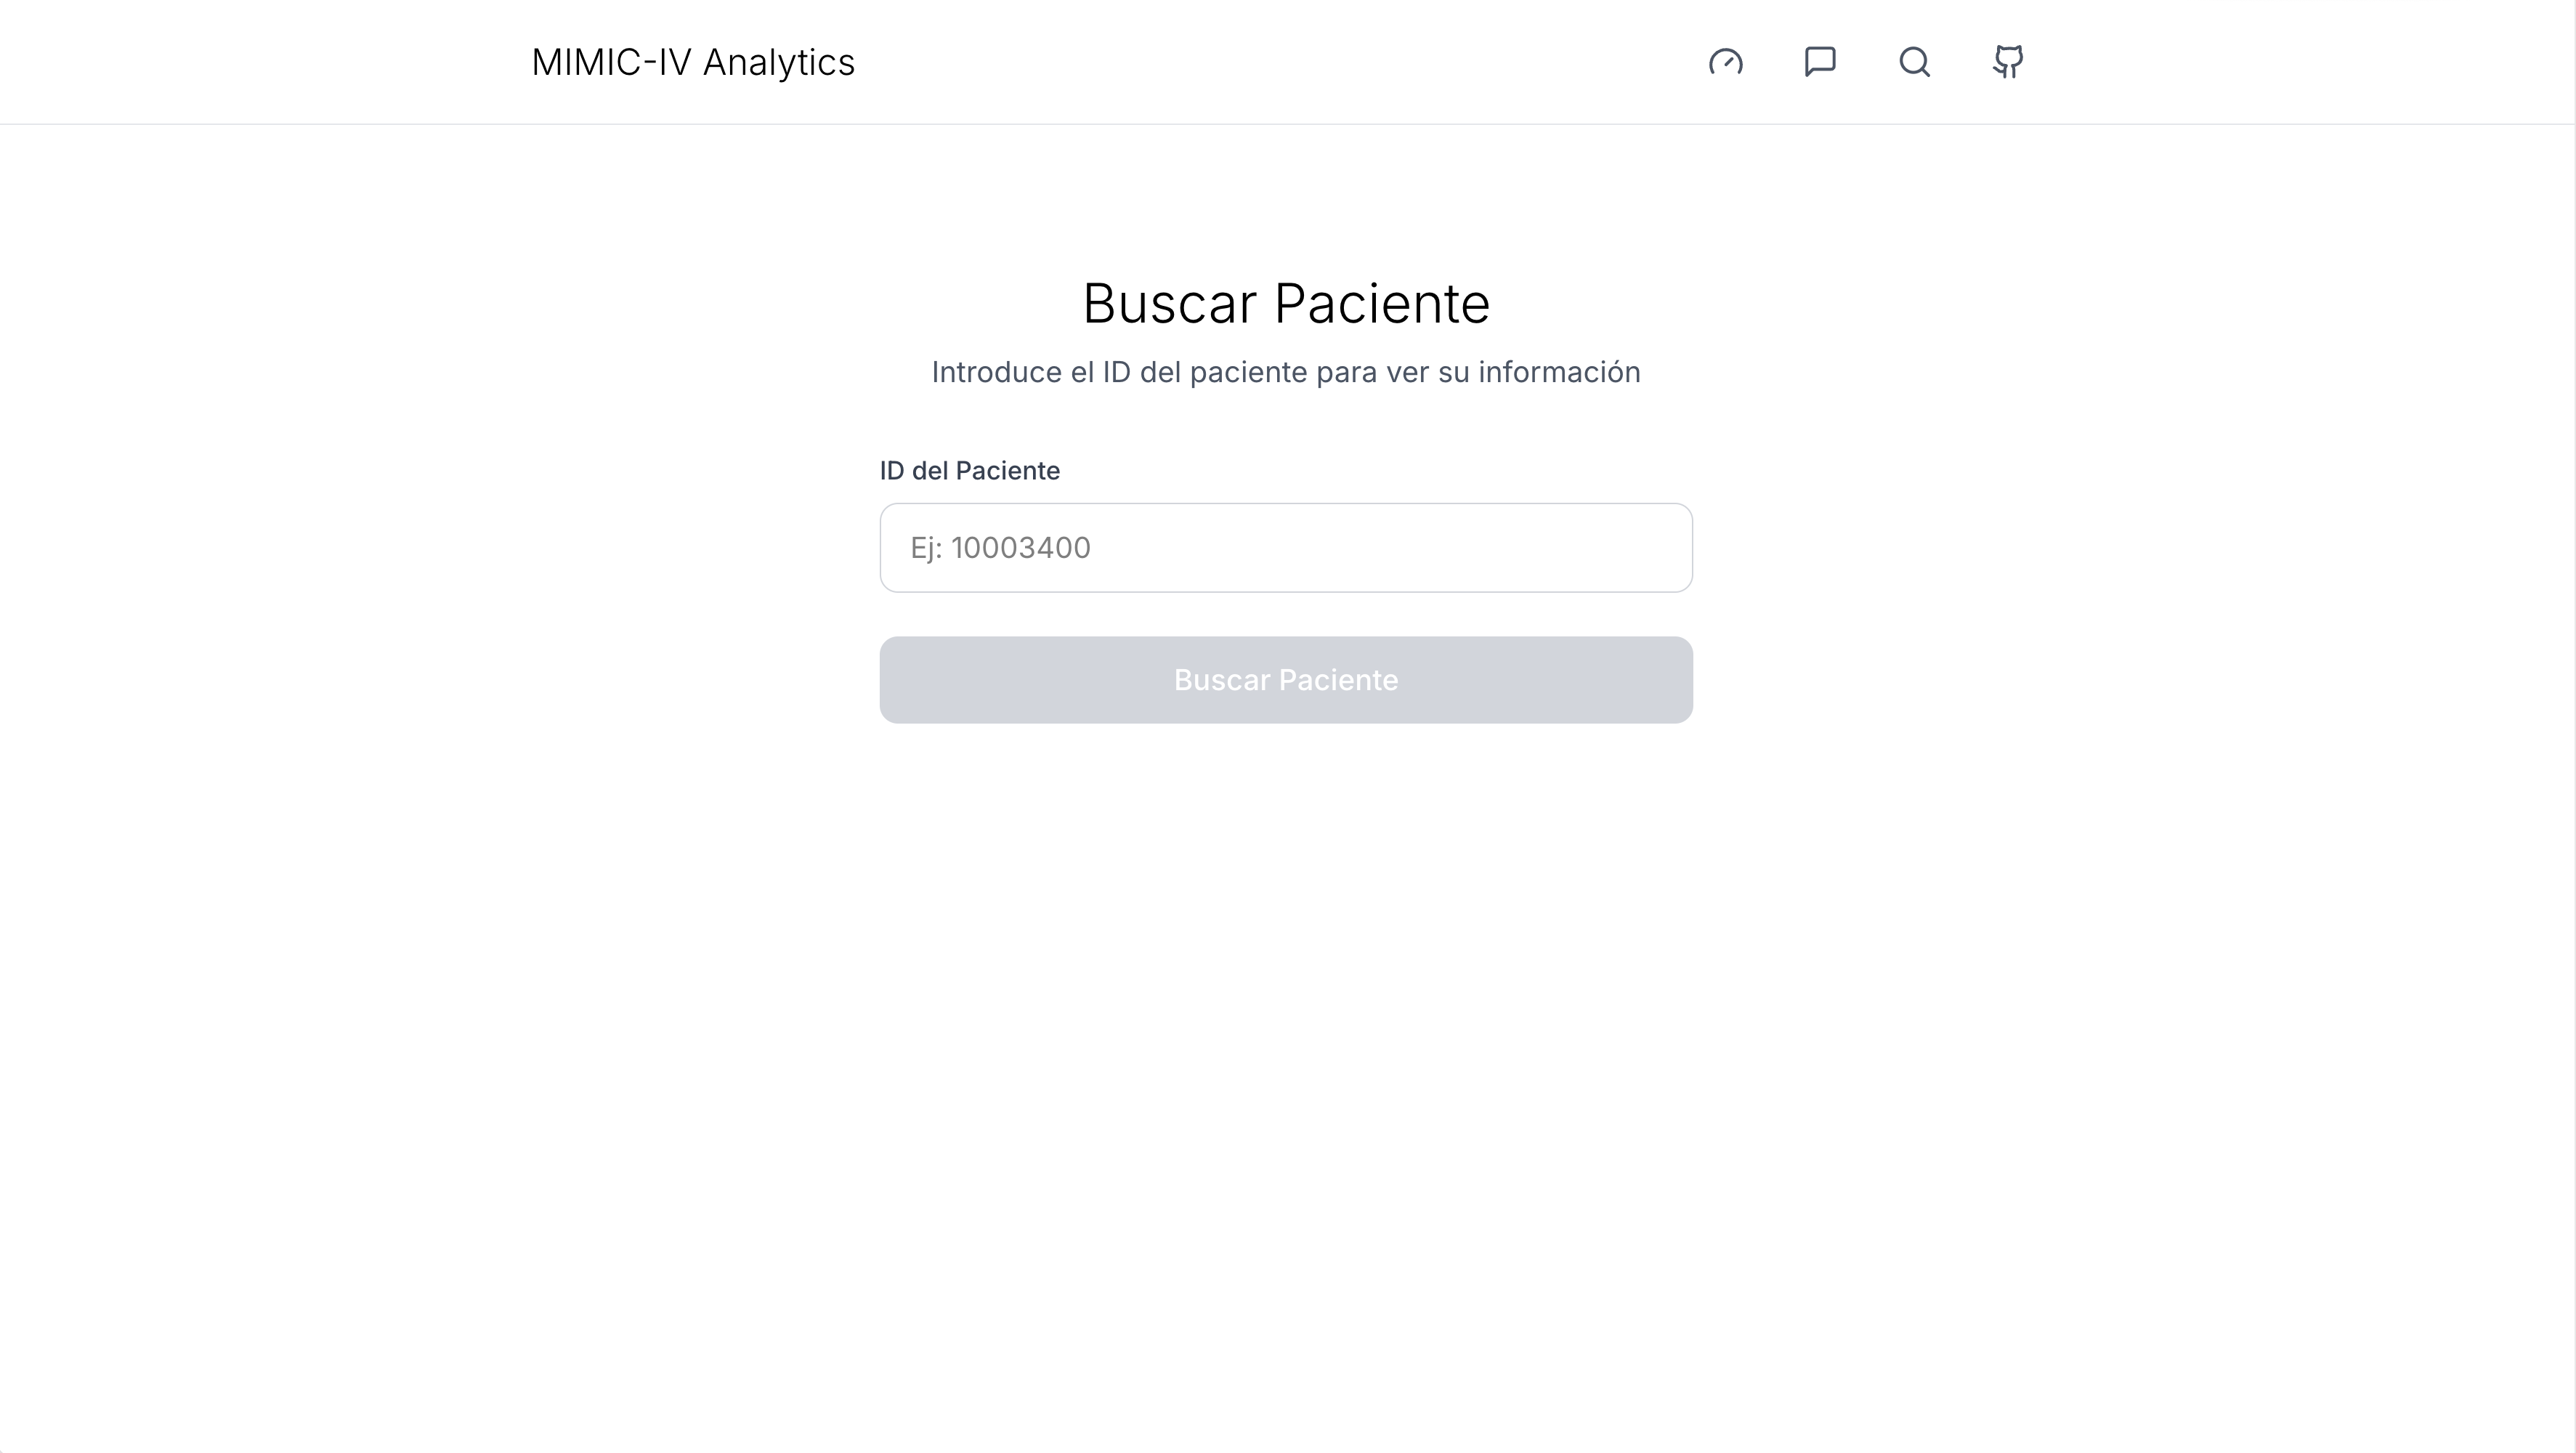
\includegraphics[width=1\textwidth]{imagenes/search.png}}
  \caption{Captura de pantalla de la página de búsqueda de pacientes.}
  \label{fig:search}
\end{figure}

\subsubsection{Página del paciente individual}

Al aterrizar en una de estas páginas, lo que hacemos es obtener el ID del paciente (\texttt{subject\_id}) de la URL, y lo envíamos al backend, a la ruta \texttt{/api/patients/\$\{id\}}. Este nos devuelve absolutamente toda la información relacionada con el paciente que necesitamos, por lo que puede tardar varios segundos en responder. Una vez con los datos, los mostramos de forma estructurada y visualmente agradable. A continuación se explican las tres secciones distintas en las que se ha organizado la información, las cuales han sido implementadas como componentes distintos que reciben los datos que necesitan de la página padre.

En primer lugar encontramos una sección con la información demográfica básica del paciente: género, edad, idioma, raza, etc. Implementado en el componente React \texttt{PatientBasicInfo}.

En segundo lugar, una sección en la que se muestra un resumen del paciente realizada con Inteligencia Artificial. El funcionamiento es el siguiente: una vez se reciben todos los datos del paciente y se carga la página, automáticamente el componente \texttt{PatientAISummary} llama a otro endpoint del backend \texttt{/api/summary/patient} y le envía todos los datos del paciente, para que se llame al LLM y se obtenga el resumen del historial. De esta forma, enviando los datos directamente y no el ID del paciente, nos ahorramos el tiempo de espera de volver a agregar toda información.

En tercer lugar tenemos el grueso de la información, en el componente \texttt{PatientAdmissions}. En el mediante desplegables, vemos un listado de todos los ingresos que ha tenido el paciente, junto a algunas estadísticas rápidas para ver a simple vista: número de días de duración de la hospitalización, número de diagnósticos asociados a la estancia, número de procedimientos, y número de tests de laboratorio. 

Al hacer click en el desplegable, podemos ver más información del ingreso, como las fechas exactas de entrada y salida, el tipo del seguro del paciente, a dónde se trasfirió despues, etc. Además, de nuevo, a forma de desplegables, podemos ver la información detallada de los diagnósticos, procedimientos, y tests de laboratorio.

En cuanto a los últimos, se ha implementado poder filtrar los tests según su categoría (Blood Gas, Hematology, Chemistry...) o bien verlos todos a la vez. De nuevo, se muestra el listado de los tests como un listado de elementos desplegables, búscando la limpieza visual al encapsular la información y visualizar sólo los datos que se quieren ver. Cuando se hace click en uno de los tests, si éste tiene dos o más ocurrencias, se mostrará una gráfica con la evolución temporal para dicha métrica. 


\begin{figure}[H]
  \centering
  \fbox{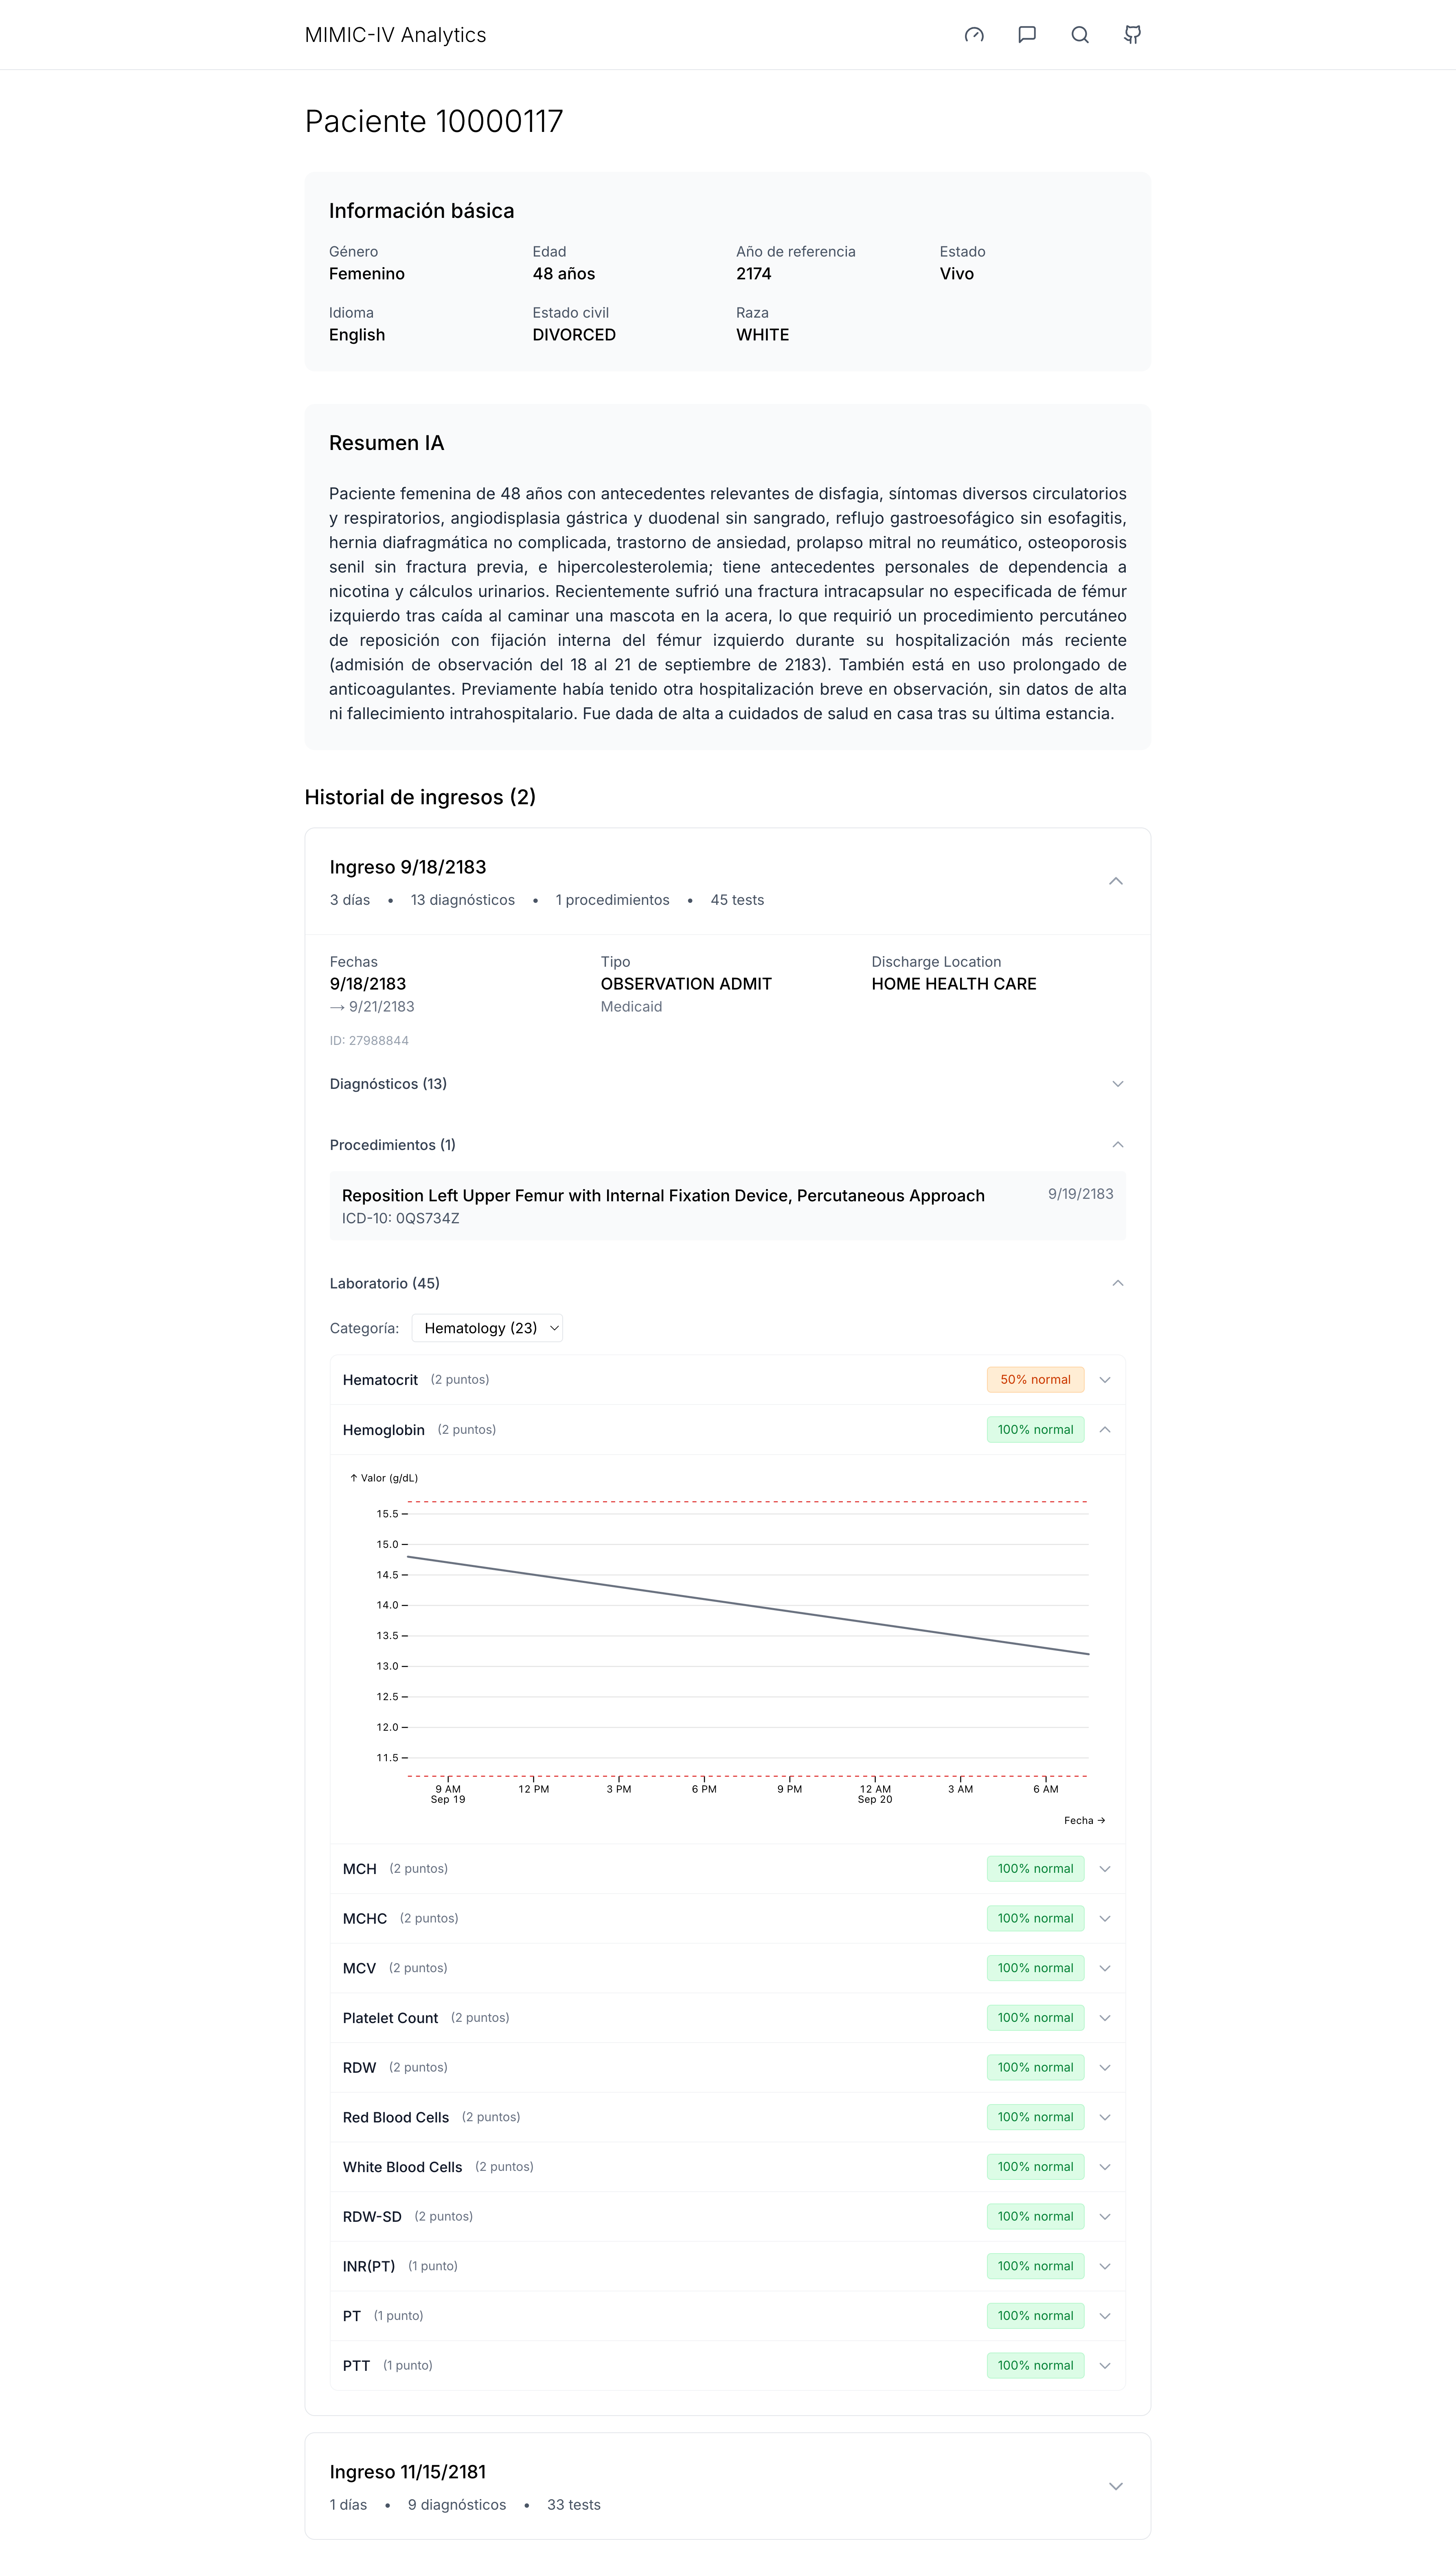
\includegraphics[width=0.9\textwidth]{imagenes/patient1.png}}
  \caption{Captura de pantalla de la página de búsqueda de pacientes.}
  \label{fig:search}
\end{figure}

%-----------------
\subsubsection{Página de gráfico: distribución por edad y género}

Ahora vamos a pasar a las visualizaciones de datos que se han implementado. El primer gráfico, realizado utilizando Observable Plot, es un Population Pyramid \cite{populationPyramid} de la distribución por edad y género, con dos variantes, una por rangos de edad, y la otra por edad específica.


\begin{figure}[H]
  \centering
  \fbox{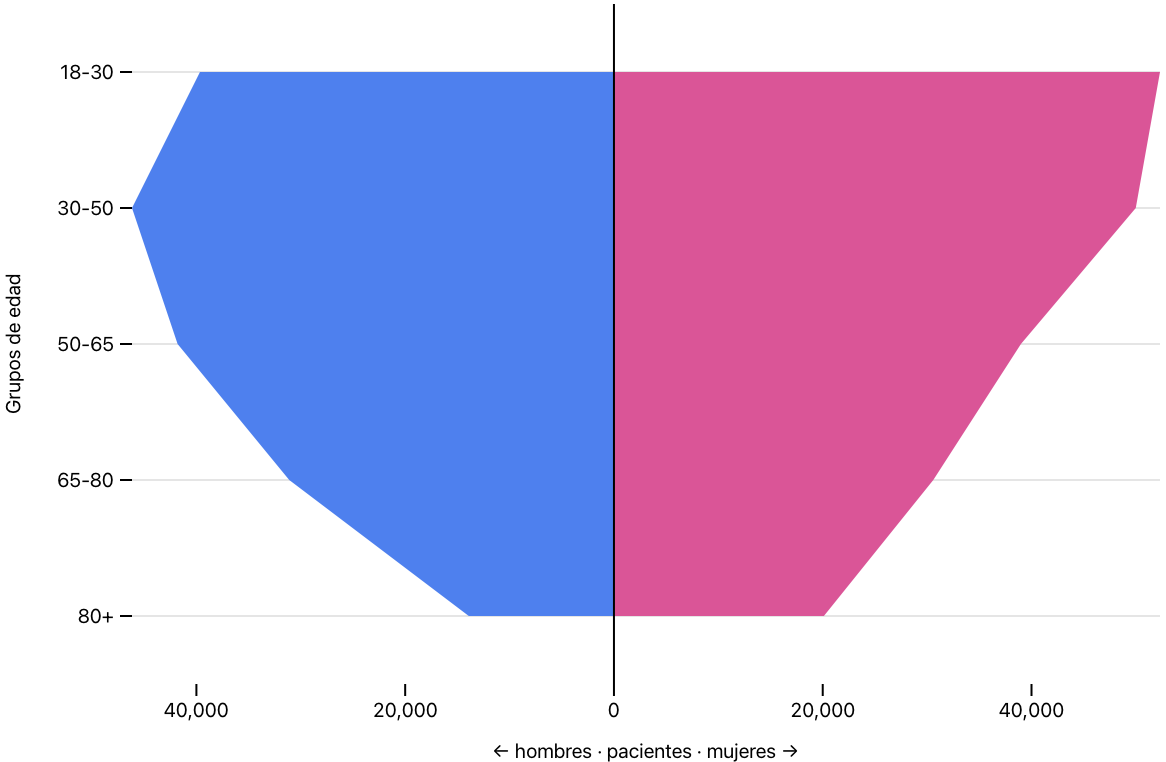
\includegraphics[width=0.65\textwidth]{imagenes/chart2.png}}
  %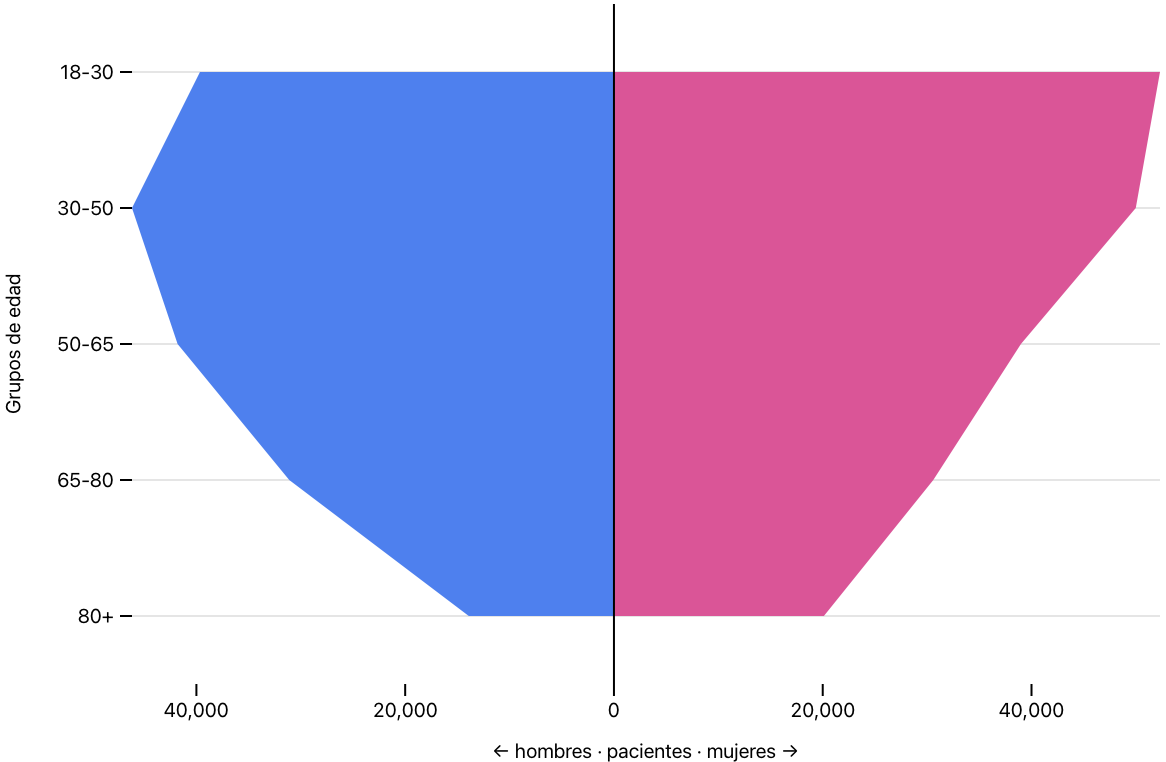
\includegraphics[width=0.65\textwidth]{imagenes/chart2.png}
  \caption{Distribución por edad y género (rangos de edad)}
  \label{fig:chart2}
\end{figure}

\begin{figure}[H]
  \centering
  \fbox{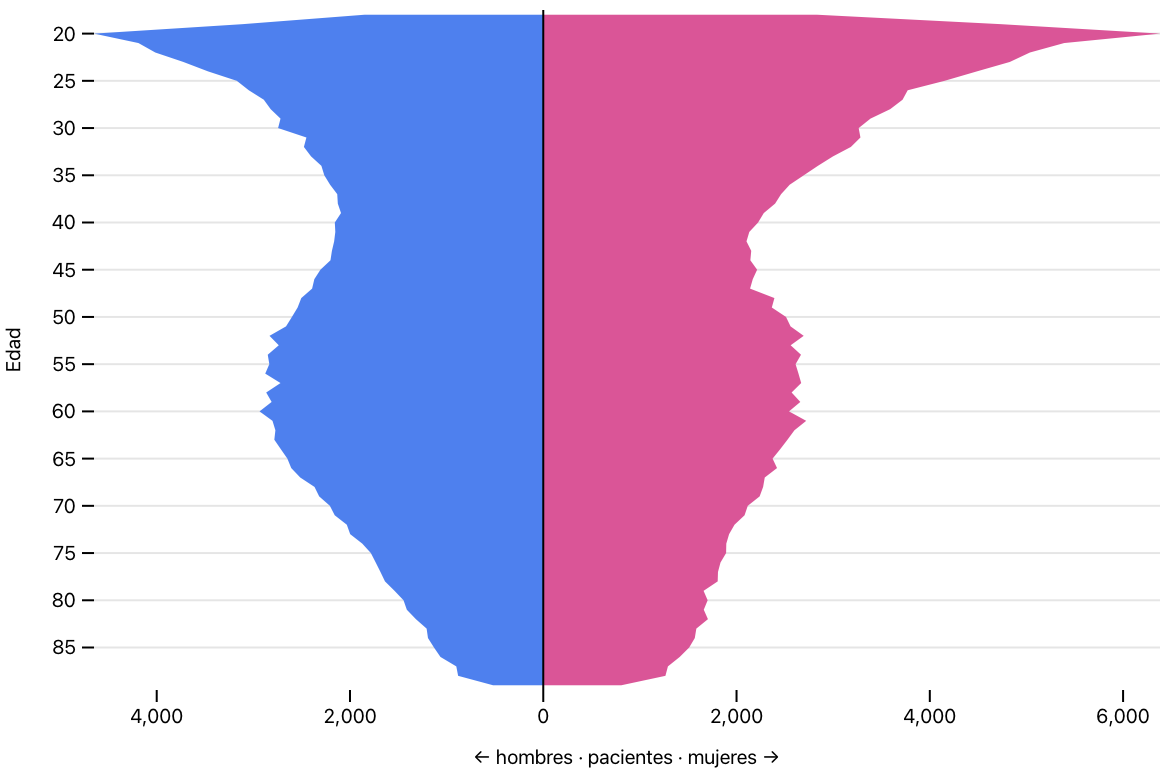
\includegraphics[width=0.65\textwidth]{imagenes/chart3.png}}
  %\includegraphics[width=0.65\textwidth]{imagenes/chart3.png}
  \caption{Distribución por edad y género}
  \label{fig:chart3}
\end{figure}


%-----------------
\subsubsection{Página de gráfico: heatmap de ingresos}

El segundo gráfico, también desarrollado con Observable Plot, consiste en un heatmap\cite{heatmap} que representa la cantidad de ingresos hospitalarios en función de la hora y la fecha, ofreciendo dos variantes. La primera muestra los ingresos distribuidos por horas y días de la semana, lo que permite identificar los periodos de mayor y menor actividad en el hospital. Durante el desarrollo se detectó una concentración anómala de ingresos a las 00:00:00, de lo que se dedujo que se trataban de registros en los que la hora real de ingreso no estaba disponible; por ello, se filtraron estos casos del gráfico principal, aunque se dejó la opción de visualizarlos mediante un botón para que el usuario pueda acceder siempre a la información completa.

La segunda variante del heatmap representa los ingresos por mes y día del mes. Aquí, el día 29 de febrero presentaba un número de ingresos significativamente inferior, lo que distorsionaba la escala de colores y oscurecía el resto de los datos. Para evitar este efecto, se optó por excluir ese día del gráfico principal y mostrar su valor de forma separada, garantizando así una visualización más precisa y homogénea del resto de los datos.


\begin{figure}[H]
  \centering
  \fbox{\includegraphics[width=0.8\textwidth]{imagenes/chart-heat-1.png}}
  %\includegraphics[width=0.8\textwidth]{imagenes/chart-heat-1.png}
  \caption{Heatmap de ingresos por hora y día de la semana.}
  \label{fig:chart-heat-1}
\end{figure}

\begin{figure}[H]
  \centering
  \fbox{\includegraphics[width=0.8\textwidth]{imagenes/chart-heat-2.png}}
  %\includegraphics[width=0.8\textwidth]{imagenes/chart-heat-2.png}
  \caption{Heatmap de ingresos por mes y día del mes.}
  \label{fig:chart-heat-2}
\end{figure}


%-----------------
\subsubsection{Página de gráfico: duración de estancias por unidad UCI}

Este gráfico, un Horizontal Bar Chart \cite{hbarchart} de Observable Plot, muestra cual es el  número de días promedio de estancia para cada unidad UCI. Se ha implementado un input para modificar el umbral mínimo de estancias, ya que hay unidades con muy pocas estancias que pueden no ser informativas. Un ejemplo es la unidad \texttt{Neurology}, que sólo tiene una estancia, y es de 28 días, muy por encima del resto. 

%Cabe destacar que pasando el cursor por encima de cada barra, se muestra el numero exacto de estancias para esa unidad.


\begin{figure}[H]
  \centering
  \fbox{\includegraphics[width=0.75\textwidth]{imagenes/chart-icu.png}}
  %\includegraphics[width=0.75\textwidth]{imagenes/chart-icu.png}
  \caption{Estancia promedio por unidad UCI}
  \label{fig:chart-icu}
\end{figure}


%-----------------
\subsubsection{Página de gráfico: medicamentos más prescritos por vía}

Esta visualización es más compleja que las anteriores, por lo que se hace uso de la librería D3. Se trata de un gráfico Sunburst interactivo \cite{sunburst}, que permite hacer zoom para moverse por la información. Se muestran los medicamentos más prescritos por vía de administración. Para este gráfico, debido a la enorme cantidad de documentos (más de 20 millones) en la colección donde se aloja esta información \texttt{hosp\_prescriptions}, en lugar de obtener los datos en cada llamada al endpoint del backend, se ha realizado una colección nueva mediante un script Python, que contiene los datos ya pre-agregados, consiguiendo así obtener los datos mucho más rápido. También se implementan unos filtros de umbral mínimo y máximo para facilitar la visualización.

\begin{figure}[H]
  \centering
  \fbox{\includegraphics[width=0.85\textwidth]{imagenes/chart-sunburst.png}}
  %\includegraphics[width=0.85\textwidth]{imagenes/chart-sunburst.png}
  \caption{Medicamentos más prescritos por vía}
  \label{fig:chart-sunburst}
\end{figure}




%-----------------
\subsubsection{Página de gráfico: número de diagnósticos por categorías}

En este caso se presenta de nuevo un gráfico interactivo realizado con D3, denominado Icicle \cite{icicle}. El gráfico muestra todos los diagnósticos, con la opción de aplicar un filtro por umbral mínimo, y están organizados jerárquicamente según la tabla \texttt{icd\_equivalencias}, mencionada previamente. Esto permite visualizar no solo los diagnósticos más frecuentes, sino también las categorías superiores que los agrupan, haciendo zoom para ver la información detallada cuando se necesite. 

Para esta visualización también se necesitó implementar un script que realiza las agregaciones necesarias y las almacena en una colección de MongoDB nueva, debido a la imposibilidad de agregar todos los datos en cada petición, el tiempo de espera era demasiado alto.

\begin{figure}[H]
  \centering
  \fbox{\includegraphics[width=0.88\textwidth]{imagenes/chart-diag.png}}
  %\includegraphics[width=0.88\textwidth]{imagenes/chart-diag.png}
  \caption{Zoomable icicle chart de diagnósticos por categoría}
  \label{fig:chart-diag}
\end{figure}

%habria q poner un ejemplo de como se puede hacer zoom? 


%-----------------
\subsubsection{Página de gráficos: flujos hospitalarios entre unidades}

Este gráfico, al igual que los dos anteriores, utiliza D3 y en este caso, se trata de un Directed Chord Diagram \cite{chord}. Para su implementación, se crea una nueva colección con los datos pre-agregados. El gráfico representa la información de \texttt{hosp\_transfers}, mostrando la cantidad de transferencias hospitalarias entre unidades. Al pasar el cursor sobre cada conexión, se ven la unidad de origen, la de destino, y el recuento de transferencias de ese tipo.


\begin{figure}[H]
  \centering
  \fbox{\includegraphics[width=0.88\textwidth]{imagenes/chart-flows.png}}
  %\includegraphics[width=0.88\textwidth]{imagenes/chart-flows.png}
  \caption{Flujos hospitalarios}
  \label{fig:chart-flows}
\end{figure}


%@todo: explicar como seria el proceso de agregar un grafico nuevo?

\subsection{Despliegue}

El frontend de la aplicación se ha desplegado públicamente utilizando la plataforma Vercel \cite{vercel}, una solución en la nube especializada en el despliegue de aplicaciones web modernas. 

Esta elección responde a varias ventajas clave para el proyecto. Por un lado, Vercel ofrece una integración nativa con Next.js, ya que es la empresa creadora de este framework. Esto permite contar con soporte optimizado y características específicas, como la optimización automática de bundles, el Server-Side Rendering (SSR) y la Static Site Generation (SSG). Además, la plataforma distribuye la aplicación a través de su red global de servidores edge, lo que garantiza tiempos de carga mínimos desde cualquier ubicación geográfica. Otro aspecto relevante es la rapidez en los despliegues, que suelen completarse en menos de 30 segundos y facilitan iteraciones ágiles durante el desarrollo. Finalmente, Vercel dispone de un plan gratuito generoso, ideal para entornos académicos y de desarrollo, que incluye 100GB de ancho de banda mensual, despliegues ilimitados y la posibilidad de utilizar un dominio personalizado.

El proceso de despliegue se gestiona de manera automática gracias a la integración por defecto entre Vercel y GitHub. Al importar el repositorio del proyecto Next.js, Vercel configura automáticamente un flujo de integración y entrega continua (CI/CD), sin necesidad de implementarlo manualmente. De este modo, cada vez que se realiza un push al repositorio principal, Vercel detecta los cambios y ejecuta los comandos de construcción de Next.js (\texttt{npm run build}), optimizando el código para producción. Durante este proceso, también se realizan las validaciones de TypeScript y ESLint configuradas en el proyecto. Una vez completada la construcción, la nueva versión se despliega de forma atómica, garantizando que no exista tiempo de inactividad, y se invalida automáticamente la caché de la CDN para asegurar que los usuarios reciban de inmediato la versión actualizada.

Gracias a este sistema, la versión en producción refleja siempre el estado más reciente del código en el repositorio principal, lo que facilita la colaboración en el desarrollo y reduce significativamente el riesgo de errores humanos durante el despliegue. La aplicación frontend está accesible en producción a través de la URL \url{https://tfg.angeloyo.com}.


\begin{figure}[H]
  \centering
  \fbox{\includegraphics[width=0.8\textwidth]{imagenes/cicd.png}}
  %\includegraphics[width=0.8\textwidth]{imagenes/cicd.png}
  \caption{Esquema del depliegue con Vercel \cite{cicdfoto}.}
  \label{fig:cicd}
\end{figure}


%
%\input{capitulos/02_EspecificacionRequisitos}
%
%\input{capitulos/03_Planificacion}
%
%\input{capitulos/04_Analisis}
%
%\input{capitulos/05_Diseno}
%
%\input{capitulos/06_Implementacion}
%
%\input{capitulos/07_Pruebas}
%
\chapter{Conclusiones y trabajo futuro}

Este proyecto ha desarrollado exitosamente una plataforma web de visualización de datos clínicos que hace accesible el conjunto de datos MIMIC-IV mediante una interfaz intuitiva y funcionalidades de inteligencia artificial. La implementación ha demostrado cómo las tecnologías modernas pueden reducir las barreras técnicas para el análisis de datos sanitarios, facilitando que profesionales sin formación tecnológica avanzada puedan extraer conocimiento valioso de bases de datos clínicas complejas.

\section{Conclusiones}

A continuación se presenta una evaluación detallada del cumplimiento de los objetivos específicos planteados al inicio del proyecto:

\textbf{OE1. Investigar sobre el problema y sus posibles soluciones (100\% completado).} Se realizó una revisión exhaustiva del estado del arte que abarcó desde las bases de datos clínicas abiertas hasta las tecnologías de visualización y los grandes modelos de lenguaje en medicina. Esta investigación, documentada en el Capítulo 2, permitió identificar la carencia de plataformas abiertas para explorar MIMIC-IV de forma accesible y justificó las decisiones tecnológicas adoptadas en el proyecto.

\textbf{OE2. Almacenar el conjunto de datos MIMIC-IV en una base de datos para realizar consultas eficientes (100\% completado).} Se migró exitosamente MIMIC-IV desde archivos CSV a MongoDB, tanto en versión completa como demo. El proceso incluyó la creación de índices optimizados y colecciones auxiliares para mejorar el rendimiento. La implementación se detalla en la Sección 3.1, donde se documenta el proceso de migración, la estructura de datos resultante y las optimizaciones aplicadas.

\textbf{OE3. Desarrollar un backend API RESTful (100\% completado).} Se implementó una API completa con FastAPI que incluye endpoints para pacientes, dashboard, visualizaciones y chat. La arquitectura modular, descrita en la Sección 3.1, facilita el mantenimiento y extensibilidad del sistema. La API está desplegada en producción y funciona de manera estable.

\textbf{OE4. Construir una plataforma web con interfaz intuitiva y visualizaciones dinámicas (100\% completado).} Se desarrolló un frontend en Next.js con TypeScript que incluye seis visualizaciones interactivas diferentes, organizadas en categorías clínicas. La plataforma, documentada en la Sección 3.2, ofrece desde gráficos básicos hasta visualizaciones complejas como diagramas sunburst y chord, todos ellos responsivos y optimizados para la interpretación clínica.

\textbf{OE5. Implementar funcionalidades con IA para consultas en lenguaje natural y resúmenes de pacientes (100\% completado).} Se integró GPT-4.1 mediante el protocolo MCP (Model Context Protocol), permitiendo consultas directas sobre la base de datos en lenguaje natural. Además, se implementó la generación automática de resúmenes de historiales clínicos. Esta funcionalidad, explicada en la Sección 3.1.2, representa una innovación técnica al utilizar uno de los estándares más recientes para la integración de LLMs con sistemas de datos.

\textbf{OE6. Configurar el entorno de producción (100\% completado).} Se desplegó exitosamente la plataforma completa: el backend mediante Cloudflare Tunnels y el frontend en Vercel con CI/CD automatizado desde GitHub. 

\textbf{OE7. Redacción de la memoria (100\% completado).} Se completó la documentación técnica del proyecto, incluyendo contexto teórico, decisiones de implementación y resultados obtenidos, siguiendo las directrices académicas establecidas.



Personalmente, me siento muy satisfecho con los resultados obtenidos en este TFG. Ha sido especialmente gratificante poder combinar mis intereses en tecnología y salud, desarrollando una herramienta que puede tener un impacto real en la democratización del acceso a datos clínicos. El aprendizaje ha sido intenso y continuo: desde dominar nuevas tecnologías hasta comprender la complejidad de los sistemas sanitarios.




El trabajo me ha permitido desarrollar significativamente mis habilidades de resolución de problemas, especialmente al enfrentar desafíos técnicos complejos como la optimización de consultas en bases de datos masivas o la implementación de visualizaciones interactivas avanzadas. También he mejorado mis capacidades de comunicación técnica, tanto en la documentación del código como en la redacción de esta memoria.


\newpage
\section{Trabajo futuro}

A partir del trabajo desarrollado, se identifican múltiples líneas de mejora y extensión que podrían implementarse en el futuro:



\textbf{Integración de módulos adicionales de MIMIC-IV.} Actualmente la plataforma utiliza los módulos \texttt{hosp} e \texttt{icu}. La incorporación de los módulos \texttt{ed} (urgencias), \texttt{note} (notas clínicas) y \texttt{cxr} (radiografías) ampliaría significativamente las posibilidades de análisis. Para el módulo de notas, sería necesario implementar técnicas avanzadas de procesamiento de lenguaje natural, mientras que las radiografías requerirían capacidades de análisis de imágenes médicas.

\textbf{Sistema de filtros temporales y de cohortes.} Implementar funcionalidades que permitan a los usuarios filtrar datos por períodos específicos, tipos de pacientes o condiciones clínicas. Esto requeriría desarrollar una interfaz de filtros avanzada y optimizar las consultas de base de datos para mantener el rendimiento con filtros complejos.

\textbf{Exportación de datos y visualizaciones.} Añadir capacidades para exportar tanto los datos consultados como las visualizaciones generadas en formatos estándar (CSV, PDF, PNG). Esta funcionalidad sería valiosa para investigadores que necesiten integrar los resultados en publicaciones o presentaciones.



%\textbf{Optimización de rendimiento para consultas complejas.} Aunque el sistema funciona correctamente, algunas consultas sobre las colecciones más grandes pueden optimizarse mediante técnicas como la agregación precomputada de estadísticas frecuentes o la implementación de cachés inteligentes para consultas recurrentes.

%\textbf{Sistema de autenticación y perfiles de usuario.} Implementar un sistema de registro y autenticación que permita a los usuarios guardar consultas favoritas, crear dashboards personalizados y mantener un historial de análisis realizados. Esto requeriría diseñar una base de datos adicional para gestionar usuarios y sus preferencias.

%\textbf{API más robusta con documentación interactiva.} Expandir la API actual con más endpoints especializados y generar documentación interactiva completa que facilite su uso por parte de desarrolladores externos que deseen integrar la plataforma en sus propios sistemas.



\textbf{Modelos predictivos especializados.} Desarrollar e integrar modelos de machine learning específicos para predicción de riesgos clínicos, como predicción de mortalidad hospitalaria, duración de estancias o riesgo de readmisión. Estos modelos podrían entrenarse directamente sobre los datos de MIMIC-IV y ofrecer predicciones explicables.

%\textbf{Asistente de análisis estadístico.} Extender las capacidades de IA para que el sistema pueda sugerir automáticamente análisis estadísticos relevantes basándose en los datos consultados, generar hipótesis de investigación y proponer visualizaciones apropiadas según el tipo de datos.

%\textbf{Integración multimodal.} Si se incorporan las imágenes del módulo CXR, desarrollar capacidades de análisis multimodal que combinen datos estructurados, texto libre y radiografías para generar resúmenes más completos de los pacientes.



%\textbf{Migración a arquitectura de microservicios.} Para facilitar el mantenimiento y escalabilidad del sistema, se podría refactorizar la aplicación hacia una arquitectura de microservicios, separando las funcionalidades de visualización, IA, y acceso a datos en servicios independientes.

\textbf{Soporte para múltiples bases de datos clínicas.} Generalizar la arquitectura para soportar otros conjuntos de datos clínicos además de MIMIC-IV, como eICU, MIMIC-III o bases de datos locales que sigan estándares como OMOP-CDM. Esto requeriría desarrollar adaptadores de datos y abstraer la lógica de acceso a datos.



%\textbf{Plataforma como servicio (SaaS).} El sistema desarrollado podría evolucionar hacia una plataforma comercial que ofrezca servicios de análisis de datos clínicos para hospitales e instituciones de investigación. Esto requeriría implementar funcionalidades empresariales como facturación, multi-tenancy y acuerdos de nivel de servicio.

\textbf{Marketplace de visualizaciones.} Crear un ecosistema donde desarrolladores puedan contribuir con nuevas visualizaciones y análisis, estableciendo una comunidad activa alrededor de la plataforma. Esto podría incluir un sistema de plugins y una tienda de extensiones.

El trabajo desarrollado sienta las bases sólidas para todas estas líneas de desarrollo futuro, habiendo demostrado la viabilidad técnica y el valor potencial de hacer accesibles los datos clínicos complejos a través de interfaces modernas e intuitivas.

\section{Enlaces del proyecto}

Para facilitar la revisión y la demostración del trabajo, se incluyen los siguientes recursos públicos:

\begin{itemize}
    \item \textbf{Demo web (frontend)}: \url{https://tfg.angeloyo.com}
    \item \textbf{Vídeo de demostración}: \url{<enlace-a-Drive>}
    \item \textbf{Repositorio de código (GitHub)}: \url{<enlace-a-GitHub>}
\end{itemize}

Estos enlaces permiten contextualizar y reproducir la funcionalidad descrita a lo largo de la memoria y servirán como apoyo visual durante la defensa del TFG.


%
%\chapter{Conclusiones y Trabajos Futuros}
%
%
%%\nocite{*}
\bibliography{bibliografia/bibliografia}\addcontentsline{toc}{chapter}{Bibliografía}
\bibliographystyle{unsrturl}
%
%\appendix
%\input{apendices/manual_usuario/manual_usuario}
%%\input{apendices/paper/paper}
%\input{glosario/entradas_glosario}
% \addcontentsline{toc}{chapter}{Glosario}
% \printglossary
\chapter*{}
\thispagestyle{empty}

\end{document}
